otoplatin\documentclass[a4paper,openright,12pt]{report}
\usepackage[spanish]{babel} % espanol
\usepackage[utf8]{inputenc} % necesario para introducir las tildes automáticamente
\usepackage[latin1]{inputenc} % acentos sin codigo
\usepackage{graphicx} % graficos
\usepackage{amsfonts}
\usepackage{hyperref}
\usepackage{amsmath}
\usepackage[mathscr]{euscript}
\usepackage{verbatim}
% si estas haciendo la tesis en B5, hay que añadir las siguientes cinco líneas.
%\setlength{\textwidth}{125mm}
%\setlength{\textheight}{195mm}
%\setlength{\oddsidemargin}{0mm}
%\setlength{\evensidemargin}{28mm}
%\setlength{\topmargin}{-5mm}

\begin{document}

%-----------------------------------------------------------------------------------------------------------------------------------------------------------------------------------------
%------------------------------ PORTADA DE LA TÉSIS --------------------------------------------------------------------------------------------------------------------------------------
%-----------------------------------------------------------------------------------------------------------------------------------------------------------------------------------------

\begin{titlepage}

\begin{center}
\vspace*{-1in}
\begin{figure}[htb]
\begin{center}

\includegraphics[width=8cm]{Logotipo_completo}
\end{center}
\end{figure}
%UNIVERSIDAD DEL PAÍS VASCO / EUSKAL HERRIKI UNIBERTSITATEA
\vspace*{0.6in}
FACULTAD DE MEDICINA Y ODONTOLOGÍA\\
\vspace*{0.15in}
DEPARTAMENTO DE NEUROCIENCIAS \\
\vspace*{0.6in}
\begin{large}
TESIS DOCTORAL:\\
\end{large}
\vspace*{0.2in}
\begin{Large}
\textbf{REVISIÓN SISTEMÁTICA Y METAANÁLISIS MULTIVARIADO DE LA EFICACIA Y SEGURIDAD DE POTENCIADORES
COGNITIVOS EN ESQUIZOFRENIA} \\
\end{Large}
\vspace*{0.3in}
\begin{large}
Doctorando: Borja Santos Zorrozúa\\
\end{large}
\vspace*{0.3in}
\rule{80mm}{0.1mm}\\
\vspace*{0.1in}
\begin{large}
Dirigida por: \\
Francisco Javier Ballesteros Rodríguez \\
\end{large}
\end{center}

\end{titlepage}

\newpage
\mbox{}
\thispagestyle{empty} % para que no se numere esta página

%-----------------------------------------------------------------------------------------------------------------------------------------------------------------------------------------
%------------------------------ DEDICATORIA ----------------------------------------------------------------------------------------------------------------------------------------------
%----------------------------------------------------------------------------------------------------------------------------------------------------------------------------------------- 

\chapter*{}
\pagenumbering{Roman} % para comenzar la numeracion de paginas en numeros romanos
\begin{flushright}
\textit{Dedicado a \\
mi familia}
\end{flushright}

%-----------------------------------------------------------------------------------------------------------------------------------------------------------------------------------------
%------------------------------ AGRADECIMIENTOS ------------------------------------------------------------------------------------------------------------------------------------------
%----------------------------------------------------------------------------------------------------------------------------------------------------------------------------------------- 

\chapter*{Agradecimientos} % si no queremos que añada la palabra "Capitulo"
\addcontentsline{toc}{chapter}{Agradecimientos} % si queremos que aparezca en el índice
\markboth{AGRADECIMIENTOS}{AGRADECIMIENTOS} % encabezado 
 
¡Muchas gracias a todos!

%-----------------------------------------------------------------------------------------------------------------------------------------------------------------------------------------
%------------------------------ RESUMEN --------------------------------------------------------------------------------------------------------------------------------------------------
%----------------------------------------------------------------------------------------------------------------------------------------------------------------------------------------- 

\chapter*{Resumen} % si no queremos que añada la palabra "Capitulo"
\addcontentsline{toc}{section}{Resumen} % si queremos que aparezca en el índice
\markboth{RESUMEN}{RESUMEN} % encabezado

Será conveniente dejarlo para cuando la tesis ya esté redactada completamente.

%-----------------------------------------------------------------------------------------------------------------------------------------------------------------------------------------
%------------------------------ ÍNDICE DE CONTENIDOS -------------------------------------------------------------------------------------------------------------------------------------
%----------------------------------------------------------------------------------------------------------------------------------------------------------------------------------------- 

\tableofcontents % indice de contenidos

%-----------------------------------------------------------------------------------------------------------------------------------------------------------------------------------------
%------------------------------ LISTA DE FIGURAS -----------------------------------------------------------------------------------------------------------------------------------------
%----------------------------------------------------------------------------------------------------------------------------------------------------------------------------------------- 

\cleardoublepage
\addcontentsline{toc}{chapter}{Lista de figuras} % para que aparezca en el indice de contenidos
\listoffigures % indice de figuras

%-----------------------------------------------------------------------------------------------------------------------------------------------------------------------------------------
%------------------------------ LISTA DE TABLAS ------------------------------------------------------------------------------------------------------------------------------------------
%----------------------------------------------------------------------------------------------------------------------------------------------------------------------------------------- 

\cleardoublepage
\addcontentsline{toc}{chapter}{Lista de tablas} % para que aparezca en el indice de contenidos
\listoftables % indice de tablas

%-----------------------------------------------------------------------------------------------------------------------------------------------------------------------------------------
%---------------------------------------------------------------- CAPÍTULO 1: INTRODUCCIÓN -----------------------------------------------------------------------------------------------
%----------------------------------------------------------------------------------------------------------------------------------------------------------------------------------------- 
\pagestyle{myheadings}
\markright{\textit{Capítulo 1: Introducción.}}
\chapter{Introducción}\label{cap.introduccion}
\pagenumbering{arabic} % para empezar la numeración con números
\section{Planteamiento del problema}
Hoy en día dentro del campo de la investigación científica, se trabaja con una cantidad ingente de información. Esto se traduce en un número enorme de publicaciones dentro de cualquier área y tema, como el que nos ocupa. Potenciadores cognitivos en pacientes con esquizofrenia.

A través de una revisión sistemática se intenta poner en común toda la información relacionada con un tema determinado. Se define como revisión sistemática la metodología necesaria para poder combinar toda la información existente que se ajuste a una serie de preguntas previamente establecidas, para poder dar respuesta a una determinada pregunta \cite{Cochrane_man}. El método que se aplique a una determinada búsqueda tiene que estar bien especificado puesto que el motivo de dicha búsqueda es el de dar una respuesta lo menos sesgada posible en aras de proporcionar las conclusiones más fiables posibles. Se caracterizan por tener:
\begin{itemize}
\item[i)] Una serie de objetivos claramente especificados y unos criterios de búsqueda de estudios establecidos previamente.
\item[ii)] Una metodología reproducible.
\item[iii)]Una búsqueda que trate de encontrar todos los estudios que cumplan los criterios de elegibilidad.
\item[iv)] Capacidad de poder evaluar la validez de cada uno de los estudio incluidos.
\item[v)] Proporcione de una manera sistemática la presentación y síntesis de los resultados de cada uno de los estudios incluidos.
\end{itemize}

Una vez seleccionada la información y finalizada la revisión sistemática, es necesario utilizar herramientas estadísticas para poder poner analizar la información obtenida. Esta herramienta recibe el nombre de metaanálisis \cite{Cochrane_man}.

Tras introducir la técnica que se va a emplear en este trabajo de tesis doctoral, hemos de pasar a introducir el tema científico sobre el que van a versar los estudios utilizados en este trabajo. La utilización de potenciadores cognitivos en pacientes con esquizofrenia.

La esquizofrenia es una enfermedad mental que presenta síntomas positivos, negativos, alteraciones cognitivas y trastornos del ánimo \cite{DSMIV1994}, es considerada la enfermedad mental más grave y persistente. Aunque los antipsicóticos de segunda generación proporcionan un efecto positivo a la hora de tratar las alteraciones cognitivas si los comparamos con los de primera generación, el tamaño de dicho efecto no parece que tenga relevancia clínica. De esta manera la ausencia de un tratamiento adecuad es uno de los mayores problemas a la hora de tratar a los enfermos.

Los estudios neuropsicológicos realizados en estos enfermos, reportan alteraciones en varios aspectos relacionados con las capacidades cognitivas como son: velocidad de procesamiento, atención, memoria de trabajo, funciones ejecutivas y aprendizaje y memoria tanto en las primeras fases \cite{Zabala2009}, como en las premórbidas \cite{Reichenberg2009}. Todo esto se traduce en un detrimento de la calidad de vida y por tanto provocan una repercusión desfavorable de su funcionamiento, tanto social como laboral \cite{Green2006}.

Debido a que numerosos sistemas de neurotransmisión están relacionados con la cognición, se ha sugerido que su potenciación mediante fármacos podría se útil a la hora de tratar a este tipo de pacientes. Por lo tanto, el uso de este tipo de fármacos como coadyuvantes al tratamiento básico de la esquizofrenia, podría ser beneficioso, ya que las expectativas de los pacientes podrían verse mejoradas \cite{Harvey2009}

Sin embargo la eficacia y la seguridad de estos tratamientos sigue sin ser concluyente debido principalmente a tres problemas: la mezcla de diseños clínicos, alta heterogeneidad entre estudios y el tamaño reducido de las muestras. 

Respecto al primero de los problemas indicados, más del 30\% de los estudios son cruzados lo que puede sesgar los resultados debido al efecto ``carry-over". Este fenómeno ya ha sido detectado en la literatura \cite{Ballesteros2008} y de estar presente, forzaría a utilizar sólo el primer periodo de este tipo de estudios lo que reduce la muestra y su potencia. La inconsistencia de las medidas cognitivas y la variedad de las mismas explica el porqué del segundo problema. Finalmente, surge el tercer problema debido a que el número de pacientes reclutados tanto en ensayos cruzados como en los de grupos paralelos no es grande. La gran presencia de estudios cruzados se puede deber a la intención de mantener un control experimental alto, pero es el efecto ``carry-over" mencionado anteriormente, lo que hace que el tamaño sea reducido. Por tanto, todo ello provoca que los intervalos de confianza sean muy amplios traduciéndose en una escasa precisión a la hora de valorar los resultados de estos estudios.

Existen trabajos previos ya publicados que siguen esta línea. Hay publicados trabajos que únicamente valoran el efecto en el grupo experimental \cite{Chourinard2007}\cite{Stip2007}, que no cubren nuestros objetivos. También se han publicado estudios en los que sólo se emplean un tipo de inhibidores \cite{Ribeiz2010}, cuya meta aunque se solapa con la nuestra no es tan ambiciosa. Por último tenemos que decir que existen metaanálisis: de estudios longitudinales \cite{Szoke2008} basado en un test-retest de únco grupo, valorando las diferencias en cognición entre esquizofrenia y trastornos esquizoafectivos y psicosis afectivas \cite{Bora2009}. Por otro lado existen protocolos Cochrane: uno que no tiene nuestros mismos objetivos \cite{Singh2009} y uno protagonizado por el grupo de investigación del que formo parte que representa una parte del proyecto que aquí se presenta. 

\section{Objetivos}
El objetivo de este trabajo de tesis doctoral es la realización de una revisión sistemática y un posterior metaanálisis multivariado para valorar la eficacia y seguridad de diferentes potenciadores cognitivos, como tratamiento coadyuvante del déficit cognitivo en el espectro de la esquizofrenia. Los resultados ayudarán a dismunir la incertidumbre que existe en relación a la eficacia y seguridad de estos tratamientos en esquizofrenia.

\section{Interés científico}
Los estudios que se seleccionarán mediante el proceso de revisión sistemática, se analizarán conjuntamente mediante la técnica de metaanálisis. Estos estudios evalúan varios outcomes relacionados con aspectos cognitivos, por lo tanto el metaanálisis que se utilizará a lo largo de este trabajo será el metaanálisis multivariado.

De este modo el interes científico radicará en la utilización y desarrollo de las técnicas de metaanálisis multivariado \cite{Becker2007}, debido a la más que posible correlación entre los diferentes outcomes evaluados en los estudios \cite{Berkey1996}\cite{Arends2003}. Es esta correlación la que justifica el empleo de esta técnica ya que, empleándola conjuntamente con los estimadores del efectos asociados a cada uno de los outcomes, los tamaños del efecto conjunto, serán estimados de una manera más precisa. Ya que si se metaanalizaran por separado, estaríamos asumiendo implícitamente una independencia que muy probablemente no exista.

La puesta en práctica de técnicas metaanalíticas multivariadas, tanto en su rama frecuentista como bayesiana \cite{Jackson2010} \cite{Nam2003}, puede suponer un empuje en su divulgación ya que actualmente su uso no está tan extendido como el del metaanálisis tradicional \cite{Jackson2011}.

Por lo tanto, este trabajo tratará de aportar desarrollos metodológicos en los aspectos más delicados como puede ser la estimación de la correlación de los diferentes otucomes, tanto dentro un mismo estudio como entre los estudios (análogo a la heterogeneidad en el caso univariado). Además se utilizarán modelos particulares en el caso de que tengamos muestras pequeñas y por supuesto se tendrán en cuenta los posibles sesgos.

De este modo no sólo se aprovechará al máximo en el análisis toda la información disponible, sino que también se pretenderá comparar las diferentes técnicas de aproximación de correlaciones \cite{Ishak2008}\cite{Riley2009} tanto de manera iterativa, mediante fórmulas cerradas \cite{Wei2013} o mediante la búsqueda de distribuciones de probabilidad que se ajusten a los datos disponibles \cite{Lambert2005}.

Así mismo este trabajo de investigación puede suponer un avance en el desarrollo de funciones destinadas a análisis metaanalíticos frecuentistas y bayesianos en diferentes paquetes estadísticos habitualmente utilizados para ello: Stata \cite{Stata}, R \cite{R}, WinBUGS \cite{WinBUGS}. 

%-----------------------------------------------------------------------------------------------------------------------------------------------------------------------------------------
%-------------------------------------------------------------- CAPÍTULO 2: METODOLOGÍA --------------------------------------------------------------------------------------------------
%----------------------------------------------------------------------------------------------------------------------------------------------------------------------------------------- 
\chapter{Metodología}\label{cap.metodología}
\markright{\textit{Capítulo 2: Metodología.}}
\section{Material}
\subsection{Criterios para considerar la inclusión de los estudios.}
\subsubsection{Estudios.}

Los estudios que serán candidatos a formar parte de esta revisión sistemática y metaanálisis únicamente serán ensayos clínicos controlados y aleatorizados (RCTs) y estudios de grupos cruzados (cross-over). El motivo fundamental por el que sólo se seleccionarán estos dos tipos de estudios, es que son los estudios aleatorizados los que aportan la información con mayor calidad.

Los estudios que no se aleatorizan pueden presentar multitud de sesgos como sesgo de selección, de confusión o de información entre otros. Estos sesgos perturban el verdadero tamaño del efecto del tratamiento y en consecuencia aumentan la posibilidad de que la información que aportan sea errónea. 

\subsubsection{Participantes.}

La población diana escogida será la de enfermos de esquizofrenia según el criterio DSM-IV \cite{DSMIV1994}.

\subsubsection{Intervenciones.}

El tratamiento será antipsicótico más potenciador cognitivo en la rama tratamiento mientras que la rama control únicamente antipsicótico. El potenciador cognitivo será cualquiera de los que están recogidos en la literatura: inhibidores de acetil-colinesterasa, agonistas nicotínicos, moduladores de receptores AMPA, etc. 

Además los periodos de tratamiento que se considerarán son: hasta 3 meses, de 3 a 6 meses, de 6 meses a 1 año y de más de 1 año

\subsubsection{Resultados.}

Esta revisión sistemática y metaanálisis centrará su atención en aquellos estudios que presentes resultados tanto en variables cognitivas como en tolerancia, discontinuación del tratamiento por cualquier causa y efectos adversos derivados del tratamiento.

Como medidas de resultado de eficacia primarias se tomarán las variables cognitivas: atención y velocidad de procesamiento, funcionamiento ejecutivo, y memoria verbal o visual. En consecuencia las medidas de resultado secundarias serán las relacionadas con la tolerancia, discontinuación y presencia de efectos adversos.

Los tamaños del efecto que servirán para estimar la eficacia de cada uno de los diferentes outcomes serán continuas (diferencia de medias o diferencia estandarizada de medias) o dicotómicos (odds ratio), cuya combinación se realizará utilizando un metaanálisis multivariado de efectos aleatorios.

\subsubsection{Criterios de selección.}

Resumiendo lo mencionado anteriormente, los articulos serán incluidos en la revisión sistemática y posetrior metaanalisis siguiendo los siguiente criterios:
\begin{itemize}
\item[i)] El diseño del estudio ha de ser aleatorizado con grupo control (RCT o cross-over).
\item[ii)] La rama de tratamiento ha de ser antipsicótico más potenciador cognitivo y la rama control ha de ser antipsocótico.
\item[iii)] La población recogida deberá ser de pacientes con esquizofrenia diagnosticada.
\item[iv)] Los resultados primarios deberán guardar relación con variables cognitivas (atención y velocidad de procesamiento, funcionamiento ejecutivo, y memoria verbal o visual) y los resultados secundarios con tolerancia, discontinuación y presencia de efectos adversos.
\item[v)] No se aplicarán restricciones de idioma para poder abarcar el mayor abanico posible de publicaciones.
\end{itemize}

\subsubsection{Búsqueda de artículos.}

Para identificar los posibles estudios relacionados con el tema de la investigación y poder posteriormente incluirlos en el metaanálisis, se rastrearon las siguientes bases de datos: Cochrane (CENTRAL), Medline (Ovid MEDLINE(R) 1946 to March Week 4 2014, Ovid MEDLINE(R) In-Process & Other Non-Indexed Citations April 03, 2014,  Ovid MEDLINE(R) Daily Update April 03, 2014), Embase (Embase 1974 to 2014 Week 13), PsycINFO (PsycINFO 1806 to April Week 1 2014). Para poder abarcar una mayor cantidad de estudios y obtener una mayor calidad, no se impusieron límites idiomáticos, se emplearon filtros validados para refinar la búsqueda por estudios controlados y aleatorizados (experimentales) y se limitó la búsqueda en el tiempo desde el año 2007 hasta el 4 de abril de 2014.

Para que la replicación de esta búsqueda pueda ser realizada sin ningún tipo de problema y a fin de que el proceso de dicha búsqueda sea lo más transparente posible, en el anexo 2 se recogen los diferentes algoritmos empleados en las distintas bases de datos rastreadas.

Bli bli bli
\paragraph{párrafo1}
Blo blo blo
\newpage
\section{Métodos}
\subsection{¿Qué es el metaanálisis?}

El término \textbf{metaanálisis} fue introducido por primera vez en el campo de las ciencias de la educación \cite{Glass1976} para nombrar a todo análisis estadístico encargado de integrar los resultados obtenidos a partir de la búsqueda de información en la literatura. En el área de la medicina desde sus inicios, el metaanálisis se ha empleado mayoritariamente para combinar resultados de ensayos clínicos aleatorizados. Las revisiones puestas al día, como las que ofrece la Cochrane Database of Systematic Reviews, facilitan notablemente la realización de metaanálisis en este tipo de estudios. Hoy en día debido al incremento de estudios, no sólo de ensayos clínicos, nos podemos encontrar con metaanálisis de estudios observacionales, dosis-respuesta, evaluación de pruebas diagnósticas...  Por lo tanto, el metaanálisis es la parte estadística de cualquier revisión sistemática.

Una vez finalizado el proceso de búsqueda de los estudios, es decir, después de haber realizado una búsqueda bibliográfica reproducible,  en base a unos criterios de búsqueda determinados y una vez filtrados aquellos verdaderamente relevantes de acuerdo al tema de investigación (promotores cognitivos en esquizofrenia), debemos extrae los datos necesarios para realizar el metaanálisis.

Los datos que extraen de los diferentes estudios y que posteriormente se metaanalizarán reciben el nombre de \textbf{tamaños del efecto}, magnitud que mide cuán beneficioso es el tratamiento comparando las mediciones obtenidas en el grupo que recibe el tratamiento, frente al grupo control. Dependiendo de la naturaleza del outcome que pretende medir el beneficio del tratamiento, la escala del tamaño del efecto varía \cite{Cochrane_man}
\newline
\begin{table}[!hbt]
\begin{center}
\begin{tabular}{|c|c|c|c|c|}\hline
Continuo & Discreto & Proporciones & Tasas & Supervivencia \\\hline
MD & RR & OR proporcionales & Tasas & HR \\\hline
SMD & OR &  & Tasa relativa & \\\hline
 & RD &  &  & \\\hline
 & NNT &  &  & \\\hline
\end{tabular}
\caption{Diferentes estimadores del efecto en función del outcome de estudio.}
\end{center}
\end{table}

En este trabajo, como veremos más adelante, nos centraremos en los tamaños del efecto asociados a outcomes continuos o discretos. Una vez extraídos los datos para poder calcular el  tamaño del efecto correspondiente, es necesario obtener su \textbf{desviación estándar (SD)}, mediante diferentes fórmulas bien descritas en la literatura. Finalmente con estos datos podremos realizar el metaanálisis tradicional (univariado).

\subsection{Metaanálisis univariado.}
Este es el tipo de metaanálisis más extendido y utilizado. Es válido para metaanalizar los estimadores del tamaño del efecto de un único outcome. En función de las hipótesis que hagamos acerca de las fuentes de variabilidad, tenemos dos modalidades de metaanálisis univariado, el modelo de efectos fijos y el modelo de efectos aleatorios. Pero antes de explicar ambas técnicas, vamos a introducir la notación necesaria para la explicación:
\begin{itemize}
\item[i)] $N$: número de estudios.
\item[ii)] $\theta$: tamaño del efecto real.
\item[iii)] $\widehat{\theta}$: estimador del tamaño del efecto global.
\item[iv)] $Var_{\widehat{\theta}}$: varianza del estimador global del efecto
\item[v)] $\widehat{\theta_{i}}$: estimador del tamaño del efecto para el estudio $i$-ésimo $i\in\lbrace1,\ldots,N\rbrace$.
\item[vi)] $Var(\widehat{\theta{i}})$: varianza asociada a $\widehat{\theta_{i}}$ con $i\in\lbrace1,\ldots,N\rbrace$.
\item[vii)] $w_{i}$: peso asociado al estudio $i$-ésimo con $i\in\lbrace1,\ldots,N\rbrace$.
\item[viii)] $\tau$: heterogeneidad entre estudios.
\end{itemize}
\subsubsection{Metaanalisis de efectos fijos.}
Es el modelo de metaanálisis más sencillo, ya que establece la hipótesis de que todos los tamaños del efectos don iguales, es decir:
\begin{equation}
\theta_{1}=\theta_{2}=\ldots=\theta_{N}=\theta
\label{hip_fe_univ}
\end{equation}

Por lo tanto el modelo que sigue el metaanálisis es el siguiente
\begin{equation}
\widehat{\theta_{i}}=\theta + \epsilon_{i}
\label{mod_fe_univ}
\end{equation}

Donde $\forall i \in \lbrace1,\ldots,N\rbrace, \epsilon_{i} \sim N(0,\sigma^{2})$ representa la única fuente de variabilidad, procedente del error aleatorio del propio modelo. Por lo tanto asumiendo que los tamaños del efecto siguen una distribución normal, aplicando \ref{hip_fe_univ}} y \ref{mod_fe_univ}}} llegamos a la expresión marginal del modelo de efectos fijos unidimensional que es de la forma
\begin{equation}
\theta_{i} \sim N(\theta,\sigma^{2})
\label{marginal_fe_univ}
\end{equation}

A la hora de realizar el metaanálisis, no conviene comenzar con $\widehat{\theta}$ directamente y empezar a hacer inferencia. La mejor manera de proceder es a partir de los $\widehat{\theta_{i}}$ construir $\widehat{\theta}$ y utilizando \ref{marginal_fe_univ}, preoceder a hacer inferencia. La expresión de $\widehat{\theta}$ viene dada por:
\begin{equation}
\widehat{\theta}_{FE}=\frac{\sum_{i=1}^{N}w_{i}T_{i}}{\sum_{i=1}^{N}w_{i}}
\label{ef_fe_univ}
\end{equation}
Para obtener el estimador del efecto conjunto más preciso posible es necesario encontrar los $w_{i}$ que minimicen $Var(\widehat{\theta}_{FE})$, como se puede ver en \cite{Shadish1994} es la inversa de la varianza de cada estudio:
\begin{equation}
w_{i}=\frac{1}{Var(\widehat{\theta_{i}})},\\ i\in\lbrace1,\ldots,N\rbrace
\label{peso_fe_univ}
\end{equation}
A partir de \ref{peso_fe_univ}, ya podemos calcular la varianza de $\widehat{\theta}$ dado por \ref{ef_fe_univ}, tan necesaria para poder calcular contrastes de hipótesis y construir intervalos de confianza:
\begin{equation}
Var(\widehat{\theta}_{FE})=\frac{1}{{\sum_{i=1}^{N}w_{i}}}
\label{var_ef_fe_univ}
\end{equation}

Una vez calculados el estimador conjunto del efecto y su varianza asociada mediante \ref{ef_fe_univ} y \ref{var_ef_fe_univ} respectivamente, ya se tienen las herramientas necesarias para hacer inferencia respecto al posible valor real de $\theta$, como son los contrastes de hipótesis y el intervalo de confianza.
\paragraph{Contraste de hipótesis.}
La realización de un contraste de hipótesis consiste en decidir si nuestros datos tienen la suficiente evidencia como para aceptar o rechazar que nuestro parámetro de interés sea igual o no, a un valor determinado. Dicho valor suele ser generalmente el que determina si $\theta$ es o no es estadísticamente significativo. Por lo tanto nos enfrentaríamos a un contraste de este estilo:
\begin{equation}
\left\lbrace
  \begin{array}{l}
     $H_{0}$: $\theta$ = $c$\\
     $H_{a}$: $\theta$ = $c$ \\
  \end{array}
  \right.
\label{c_h_fe}
\end{equation}
Siendo el estadístico de prueba el siguiente:
\begin{equation}
T=\frac{(\widehat{\theta}_{FE}-c)}{sd(\widehat{\theta}_{FE})}\sim N(0,1)
\label{est_prueba_fe}
\end{equation}
Que sigue una distribución normal estándar asumiendo que la hipótesis nula es cierta.
\paragraph{Intervalo de confianza.}
Como añadidura al contraste de hipótesis, se puede construir el intervalo de confianza para el parámetro que estamos estudiando. La información que aporta este intervalo es el rango de valores que tomará $\theta$ con una determinada probabilidad fijada por el investigador. La fórmula que nos permite construirlo es la siguiente:
\begin{equation}
CI_{100(1-\alpha)\%}=( \widehat{\theta}_{FE}-Z_{\frac{\alpha}{2}}\cdot \sqrt{\frac{1}{{\sum_{i=1}^{N}w_{i}}}},\widehat{\theta}_{FE}+Z_{\frac{\alpha}{2}}\cdot \sqrt{\frac{1}{{\sum_{i=1}^{N}w_{i}}}}) 
\label{int_confianza}
\end{equation}

\subsubsection{Metaanálisis de efectos aleatorios}
La hipótesis de que todos los estudios están tratando de estimar el mismo tamaño del efecto explicada anteriormente es demasiado exigente. La razón es que asumir que todos los estudios publicados estiman el mismo tamaño del efecto, es decir que todos los estudios tienen las mismas características en cuanto a: aspectos sociodemográficos, tamaño de muestra, estado de la enfermedad,\ldots 
Esto es sumamente complicado porque en la realidad los estudios, aunque traten el mismo tema, tienen diferencias lo suficientemente importantes como para no poder asumirlos iguales. Estadísticamente esto se puede comprobar mediante el llamado test de heterogeneidad:
\paragraph{Detección de heterogeneidad entre estudios.}
\begin{equation}
\left\lbrace
  \begin{array}{l}
     $H_{0}$: $\theta_{1}$ = $\theta_{2}$=\ldots=$\theta_{k}$=$c$\\
     $H_{a}$: $\exists$ $i$\in\lbrace1,\ldots,k\rbrace \vert \theta_{i} \neq \theta_{j}, j $\in \lbrace1,\ldots,i-1,i+1,\ldots,k\rbrace$ \\
  \end{array}
  \right.
\label{test_het}
\end{equation}

Cuyo estadístico de prueba es:
\begin{equation}
Q=\sum_{i=1}^{k}w_{i}(\widehat{\theta}_{i}-\widehat{\theta}_{FE})\sim\chi_{k-1}^{2}
\label{est_prueba_het}
\end{equation}

Que sigue una distribución chi cuadrado cuyos grados de libertad son el número de estudios menos uno, siempre y cuando la hipótesis nula sea cierta.

En el momento en que al realizar este test, nos vemos obligados a rechazar $H_{0}$, tenemos otra fuente de variabilidad a tener en cuenta en el metaanálisis. Esta nueva fuente de variablidad se conoce por heterogeneidad y se denota con la letra griega $\tau$. El modelo de mataanálisis que tiene en cuenta esta nueva variabilidad, recibe el nombre de mataanálisis de efectos aleatorios y lo introduciremos nada más definir el estimador de $\tau^{2}$.
\paragraph{Estmiación de la heterogeneidad entre estudios.}
Existen diversas maneras de estimar este parámetro, pero la más extendida y que introduciremos de manera breve es la DerSimonian \& Laird \cite{DerSimonian1986}. Según su método, la heterogeneidad entre estudios se estima de la siguiente manera:\newpage
\begin{equation}
\left\lbrace
  \begin{array}{l}
     $\widehat{\tau}^{2} = 0$ si $Q \leq k-1$ \\
     $\widehat{\tau}^{2} = \dfrac{Q-(k-1)}{U}$ si $Q > k-1$
  \end{array}
  \right.
\label{tau_est}
\end{equation}}

Donde $Q$ es el estadístico de prueba del test de heterogeneidad descrito en \ref{test_het}.
\paragraph{Método de efectos aleatorios de DerSimonian \& Laird.}
Llegados a este punto en el que hemos explicado el concepto de heterogeneidad entre estudios, su detección y su cuantificación, podemos pasar a exponer y desarrollar de una manera breve el modelo de efectos aleatorios. Como se asume que cada estudio trata de estimar un tamaño del efecto diferente, tenemos para cada uno de los estudios:
\begin{equation}
\widehat{\theta_{i}}=\theta_{i}+\epsilon_{i}, i\in \lbrace1,\ldots,k\rbrace
\label{mod_re_univ}
\end{equation}

Donde $\epsilon_{i}$ es el error de ajuste del modelo y se asume que cada $\widehat{\theta_{i}}$ sigue una distribución normal, $\widehat{\theta_{i}}\sim N(\theta_{i},\sigma_{i}^{2})$ para cada $i$.
La modelización de la heterogeneidad entre estudios se basa en la suposición de que el conjunto de todos los $\theta_{i}$ de los estudios conforman una muestra aleatoria de una población de tamaños del efecto cuya distribución es normal. Esta distribución normal es la siguiente:
\begin{equation}
\theta_{i}\sim N(\theta,\tau^{2}), i \in \lbrace1,\ldots,k\rbrace
\label{het_re_sim}
\end{equation}

De esta manera, quedan reflejadas las dos fuentes de variación consideradas, que no son otras que el error sistemático de cualquier modelo y la heterogeneidad entre estudios. Se puede apreciar que son las varianzas de las distribuciones mencionadas en \ref{mod_re_univ}} y \ref{het_re_sim}} respectivamente.
Ya sólo nos queda construir el estimador del tamaño del efecto conjunto y su respectiva varianza. De acuerdo con \cite{DerSimonian1986}, las variables necesarias para su construcción son: $Q$, $\widehat{\theta_{i}}$ y $w_{i}=\frac{1}{Var(\widehat{\theta_{i}}}$. Mediante el método de los minimos cuadrados, se obtienen las siguientes fórmulas:
\begin{equation}
\widehat{\theta}_{RE}=\frac{\sum_{i=1}^{k}w_{i}^{\ast}\cdot\widehat{\theta_{i}}}{\sum_{i=1}^{k}w_{i}^{\ast}}
\label{est_ef_re_mod}
\end{equation}}
\begin{equation}
w_{i}^{\ast}=\frac{1}{(w_{i}+\tau^{2})}
\label{peso_re_mod}
\end{equation}

Que son los estimadores del tamaño del efecto conjunto \ref{est_ef_re_mod} y la estimación del peso de cada uno de los estudios incluidos en el metaanálisis \ref{peso_re_mod}}. Como el error estándar asintótico de $\widehat{\theta}$ es exactamente $(\sum_{i=1}^{k}w_{i}^{\ast}})^\frac{1}{2}$ tenemos que distribución marginal de el estimador del tamaño del efecto conjunto es:
\begin{equation}
\widehat{\theta}_{RE}\sim N(\theta,\sigma^{2}+\tau^{2})
\label{dist_mar_re_mod}
\end{equation}
\paragraph{Contraste de hipótesis.}
El procedimiento es exactamente el mismo que en el caso de efectos fijos, la única diferencia va a estar en que el estimador del tamaño del efecto conjunto y el valor de la desviación estándar serán diferentes, pero la composición del contraste es la misma que en \ref{c_h_fe}.
\paragraph{Intervalo de confianza.}
Al igual que en el modelo de efectos aleatorios, lo único necesario para construir el intervalo es: el estimador del tamaño del efecto conjunto, su error estándar y el nivel de significación deseado (para calcular el valor de $Z$). Con lo cual la fórmula es la misma que en \ref{int_confianza}.
\subsubsection{Diferencias entre el método de efectos fijos y el método de efectos aleatorios.}
Las principales diferencias entre ambos modelos son las siguientes:
\begin{itemize}
\item[i)] \textbf{Desviación estándar:} $\widehat{\theta}_{RE}\geq\widehat{\theta}_{FE}$
\item[ii)] \textbf{Aplicabilidad:} El método de efectos aleatorios es el mas extendido en la literatura.
\item[iii)] \textbf{Generalización de resultados:} El resultado de un metaanalisis de efectos fijos, únicamente es extrapolable a estudios de características idénticas a los incluidos en el análisis. En cambio, el obtenido de un metaanálisis de efectos aleatorios es generalizable a cualquier estudio que evalúe el mismo outcome de interés.
\end{itemize}
Por lo tanto debido a: \textbf{i)}, \textbf{ii)} y \textbf{iii)}, se deduce que el método de efectos aleatorios es: más conservador, tiene una mayor capacidad de aplicabilidad y permite una mayor generalización respectivamente. Finalmente decir que cuando no hay una presencia estadísticamente significativa de heterogeneidad, $\tau^{2}=0$, se deduce a partir de la fórmula de ponderación del método de efectos aleatorios, que ambos métodos coinciden. Esta una razón más por la que se prefiere el método de efectos aleatorios al de efectos fijos. 
\newpage
\subsection{Metaanalisis multivariado.}
\subsubsection{Motivación}
Muchas veces los investigadores que llevan a cabo un ensayo clínico aleatorizado tienen la oportunidad de poder medir distintas variables durante el estudio. Por esta razón no es difícil encontrarse durante la etapa de búsqueda de una revisión sistemática, con estudios con varios outcomes de interés primario. En esta situación el responsable del metaanálisis de la revisión sistemática debe encontrar la mejor técnica para analizar los datos ya que de este modo obtendrá los resultados más ajustados y en consecuencia, unas conclusiones más ajustadas a la información recogida.
Precisamente por esta razón se han venido desarrollando diferentes técnicas de análisis que introduciremos brevemente y que debido a sus limitacione se han ido sustituyendo por otras. De este modo nos pondremos en antecedentes para abordar el objetivo principal de esta tesis, la estimación más correcta de la correlación entre los outcomes analizados.
\subsubsection{Ventajas sobre el modelo univariado.}
Una de las maneras más extendidas de enfrentarse a un metaanálisis multivariado, es hacerlo desde una perspectiva univariada. Esto se debe a que estas técnicas están, debido al tiempo que llevan establecidas, más extendidas y ademas es la manera más fácil de metaanalizar datos.
Siguiendo la idea de que los efectos a medir rara vez son univariados \cite{Eysenck1994} los metaanálisis que involucran múltiples efectos en en los estudios deben de analizarse con todos los outcomes simultáneamente. Está muy bien descrito en la literatura, que cualquier aproximación multivariada es mejor que la univariada tradicional. En el caso de analizar dos variables simultáneamente, Riley y colaboradores, demostraron algebraicamente que efectivamente, la aproximación bivariada es más exacta que la univariada \cite{Riley2007}. Este fenómeno se generaliza de manera empírica al escenario con más de dos variables de resultado.
Las principales ventajas del modelo multivariado son las siguientes:
\paragraph{i) Hipótesis de partida más flexibles.} Cuando en un mismo estudio se recogen varias variables, es prácticamente imposible asumir su independencia \cite{Nam2003}\cite{Jackson2011}\cite{Riley2007} con lo que analizarlas por separado no es la opción más adecuada.
\paragraph{ii) Precisión de los resultados.} Al tener en cuenta la correlación existente entre las variables de resultado de los estudios, los estimadores del efecto conjunto están más próximos a la realidad y además quedan descritas las relaciones existentes entre los diferentes estimadores \cite{Jackson2011}. El fenómeno que permite esta mejoría en la calidad de los estimadores recibe el nombre de \textbf{borrow of strength} introducido por \cite{Higgins1996} y consiste en que al incluirse todos los outcomes a la vez y al estar correlados (en mayor o menor medida), contribuyen a la estimación del resto de tamaños del efecto (en mayor o en menor medida)\cite{Nam2003}\cite{Mavridis2011}. Esta diferencia en la calidad de los estimadores se traduce en un error estándar menor \cite{Riley2007}\cite{Jackson2011}, además también se obtienen estimadores de la varianza entre estudios con un MSE menor \cite{Jackson2011}. Finalmente gracias a la intervención de la correlación en el modelo se pueden calcular regiones de confianza, generalización del intervalo de confianza, para el conjunto de estimadores \cite{Jackson2011} cuya representación gráfica es perfectamente posible para metaanálisis de dos y tres variables.
\paragraph{iii) Simplicidad del modelo.} Posiblemente sea una de las mayores ventajas ya que el metaanálisis multivariado es capaz de estimar en una sola etapa \cite{Jackson2011} y de una manera mucho más sencilla que modelos anteriores basados en modelos mixtos \cite{Berkey1996}\cite{Berkey1998}. Además otra característica de su simplicidad es su flexibilidad en el sentido de que el modelo se puede adaptar con facilidad a multitud de escenarios \cite{Nam2003}. Por otra parte sus resultados siguen siendo fiables aun con un tamaño de muestra reducido \cite{Nam2003} lo que no ocurre con la aproximación mediante modelos mixtos, ya que estos heredan los problemas de los modelos lineales generalizados con respecto a tamaños reducidos de muestra.
\paragraph{iv) Potencial contra el sesgo de selección de resultados.} Es bien sabido que el sesgo de publicación es una de las mayores limitaciones a las que se enfrenta el metaanálisis y es consecuencia de que no todos los estudios son publicados y por tanto el estimador obtenido no se ajuste a la realidad. Pero el modelo multivariante es sensible a este problema, ya que s no se han reportado determinados outcomes por los motivos que sean, el resto de información contenida en las variables recogidas, ayuda a intentar llenar el hueco dejado por la no publicada \cite{Riley2007}.
\paragraph{v) Aplicabilidad.} El modelo multivariado no impone restricciones en los outcomes, es decir, que mientras estén relacionadas pueden ser de cualquier tipo y naturaleza. Por lo tanto, esta técnica puede aplicarse a multitud de diseños diferentes como: metaanálisis de pruebas diagnósticas (sensibilidad y especificidad) \cite{Jackson2011}, estudios observacionales \cite{Jackson2011}, ensayos clínicos controlados \cite{Jackson2011}\cite{Nam2003}, estudios donde se comparan varios tratamientos teniendo en consecuencia varias ramas de tratamiento (metaanálisis en red) \cite{Jackson2011}\cite{Nam2003} o estudios de medidas repetidas (mismo outcome medido en diferentes tiempos).
\newpage
\subsubsection{Introducción del modelo}
Una vez introducidas la motivación y las ventajas del metaanálisis multivariado frente a la aproximación univariada, el siguiente punto es el de introducir de manera formal el modelo de metaanálisis multivariado. Pero al igual que cuando se definió el metaanálisis univariado, vamos a exponer la notación que se empleará en el desarrollo del método.
\begin{itemize}
\item[i)] $N$: Número de estudios.
\item[ii)] $K$: Número de outcomes.
\item[iii)] $\theta_{ij}, \left(i,j\left) \in \lbrace 1,\ldots,N \rbrace \times \lbrace 1,\ldots,K\rbrace$ y $\mathtbf{\theta}$ tamaño real del efecto de la variable $j$-ésima del $i$-ésimo estudio y el vector de tamaños reales del efecto.
\item[iv)] $\widehat{\theta_{ij}}$, $Var(\widehat{\theta_{ij}})$ y $\mathbf{\widehat{\theta_{i}}}$ el estimador del tamaño del efecto de la $j$-ésima variable del $i$-ésimo estudio, su correspondiente varianza y el vector de estimadores del efecto del $i$-ésimo estudio.
\item[iv)] $\rho_{lm}^{n}, (l,m)\in \lbrace 1,\ldots,K\rbrace \times \lbrace 1,\ldots,K\rbrace$ y $\mathbf{S_i}}$ con $i \in \lbrace 1, \ldots, N\rbrace$ la correlación existente entre las variables $l$-ésima y $m$-ésima del $n$-ésimo estudio y la matriz de varianzas-covarianzas del $i$-ésimo estudio respectivamente.
\item[v)] $\tau_{i}$ y $\mathbf{T}$ la heterogeneidad entre estudios asociada a la variable $i$-ésima y la matriz de heterogeneidades respectivamente.
\end{itemize}
Al igual que en el caso multivariado, existe un método de efectos fijos y un método de efectos aleatorios. De la misma manera que en el caso univariado se tiene un test de hipótesis para evaluar la presencia de heterogeneidad \ref{est_prueba_het}, existe una generalización para el caso multivariado en el que se trata de probar si existe heterogeneidad o no cuya hipótesis nula es $H_{0}: \mathbf{T}=\mathbf{0}$ pero es necesario conocer todas las mtrices $\mathbf{S_i}}$, lo cual sólo es posible cuando podemos recuperar los datos individuales, cosa muy poco probable \cite{Ritz2008}. 

Por lo tanto este trabajo se va a centrar en el modelo de efectos aleatorios ya que las diferencias entre éste y el de efectos fijos son todavía más pronunciadas ya que si en el caso univariado la hipótesis de que todos los estudios medían el mismo tamaño del efecto, asumirlo en un entorno de varios outcomes en cada estudio, es todavía más restrictivo y además en el supuesto de que no existiera heterogeneidad, ocurriría lo mismo que con el metaanalisis univariado, que ambos modelos coincidirían. 
El modelo está compuesto de dos partes \textbf{inter-estudios} e \textbf{intra-estudios}.
\subsubsection{Parte inter-estiduios}
Como se ha establecido antes, vamos a tener $N$ estudios con $K$ variables de resultado en cada uno de ellos, lo que hace que para cada estudio tengamos dos vectores de longitud $K$, uno que recogerá los verdaderos tamaños del efecto y otro que recogerá las estimaciones de los mismos. 

Si bien cuando trabajamos con un único outcome asumimos una distribución normal $\widehat{\theta_{i}}\sim N(\theta_{i},\sigma_{i}^{2})$, ahora vamos a asumir que el vector $\mathbf{\widehat{\theta_{i}}}$ va a seguir una \textbf{distribución normal multivariante}, cuya media será el vector $\mathtbf{\theta}$ y tendrá como matriz de varianzas covarianzas a $\mathbf{S_i}}$. La fórmula que describe a esta parte del modelo es la siguiente:
\begin{equation}
\left( \begin{array}{c}
 \widehat{\theta_{i1}} \\
 \widehat{\theta_{i2}} \\
 \vdots \\
 \widehat{\theta_{ik}}
\end{array} \right) 
\sim \mathbf{NMV}\left( 
\left( \begin{array}{c}
 \theta_{i1}} \\
 \theta_{i2}} \\
 \vdots \\
 \theta_{ik}}
\end{array} \right), 
\left( \begin{array}{cccc}
 \sigma_{1,i}^{2} &  \rho_{1,2}^{i}\sigma_{1,i}\sigma_{2,i} & \ldots & \rho_{1,k}^{i}\sigma_{1,i}\sigma_{k,i}\\
 \rho_{2,1}^{i}\sigma_{2,i}\sigma_{1,i}  &  \sigma_{2,i}^{2} & \ldots & \rho_{2,k}^{i}\sigma_{2,i}\sigma_{k,i}\\
 \vdots & \vdots & \ddots & \vdots\\
 \rho_{k,1}^{i}\sigma_{k}\sigma_{1} & \rho_{k,2}^{i}\sigma_{k}\sigma_{2} & \ldots & \sigma_{k,i}^{2}
\end{array} \right)\right) 
\label{re_multi_within}
\end{equation}

Los elementos de la diagonal de $\mathbf{S_i}}$ son las varianzas de los diferentes estimadores del tamaño del efecto y se calculan de igual manera que en el caso univariado. Los elementos que no se estiman en el modelo anterior son los que se encuentran fuera de la diagonal, que son las covarianzas entre los diferentes outcomes del estudio $i$-ésimo. 

Para estimarlos es necesario conocer tanto las desviaciones estándar (que siempre conocemos) de los estimadores como la correlación (que no siempre disponemos) existente entre las diferentes variables de resultado.
\subsubsection{Parte intra-estudios}
Siguiendo la idea de que es muy poco probable que todos los estudios midan el mismo efecto, ya que eso implicaría que las condiciones de todos los estudios incluidos fueran las mismas, en el escenario multivariado es de vital importancia permitir que los efectos varíen entre estudios sobre todo porque al haber más outcomes, todavía es más difícil que se cumplan las hipótesis del modelo de efectos fijos.

De este modo deberemos trasladar las ideas del modelo univariado al marco multivariado. La manera más fácil de hacerlo es entender que ya no vamos a trabajar con $N$ estimadores sino con 
$N$ vectores de estimadores de longitud $K_{i}, i \in \left\lbrace 1, \ldots, N \right\rbrace$. Al trabajar con vectores ya no podemos emplear distribuciones de probabilidad univariadas en nuestro modelo, lo que ya hemos hecho en el apartado anterior al definir \ref{re_multi_within}. 

Como en el metaanálisis univariado de efectos aleatorios asumíamos que los efectos formaban una muestra aleatoria de una población de tamaños del efecto cuya distribución era normal, lo que vamos a asumir en el caso multivariado es lo mismo. Por lo tanto los vectores de tamaños del efecto formarán una muestra aleatoria de la población de todos los posibles vectores de efectos y para seguir con la generalización, la distribución que la regirá será una distribución normal multivariante. 

Para terminar la construcción de esta parte del modelo necesitamos establecer el vector de medias y la matriz de varianzas-covarianzas de la distribución, las cuales serán $\mathtbf{\theta}$ y $\mathbf{T}$ respectivamente, generalizaciones del verdadero tamaño del efecto y de la heterogeneidad entre estudios definidos en \ref{het_re_sim}. La fórmula que describe a la parte intra-estudios del metaanálisis multivariado es la siguiente:
\begin{equation}
\left( \begin{array}{c}
 \theta_{i1} \\
 \theta_{i2} \\
 \vdots \\
 \theta_{ik}
\end{array} \right) 
\sim \mathbf{NMV}\left( 
\left( \begin{array}{c}
 \theta_{1}} \\
 \theta_{2}} \\
 \vdots \\
 \theta_{k}}
\end{array} \right), 
\left( \begin{array}{cccc}
 \tau_{1}^{2} &  \kappa_{1,2}\tau_{1}\tau_{2} & \ldots & \kappa_{1,k}\tau_{1}\kappa_{k}\\
 \kappa_{2,1}\tau_{2}\tau_{1}  &  \tau_{2}^{2} & \ldots & \kappa_{2,k}\tau_{2}\tau_{k}\\
 \vdots & \vdots & \ddots & \vdots\\
 \kappa_{k,1}\tau_{k}\tau_{1} & \kappa_{k,2}\tau_{k}\tau_{2} & \ldots & \tau_{k}^{2}
\end{array} \right)\right) 
\label{re_multi_between}
\end{equation}

\subsubsection{Modelo marginal}
Introducidas tanto la sección del modelo asociada a la parte inter-estudios la que modela la parte intra-estudios, ya tenemos construido totalmente el modelo que describe el metaanálisis multivariado de efectos aleatorios y podemos presentar el modelo marginal:
\begin{equation}
\mathbf{\widehat{\theta_{i}}} \sim \mathbf{N}(\mathbf{\theta},\mathbf{S_{i}}+\mathbf{T})
\label{re_multi_marginal}
\end{equation}

Donde los $\mathbf{\widehat{\theta_{i}}}$ se asumen independientes entre si al proceder de diferentes estudios. Los parámetros a estimar con la ayuda del modelo son $\mathbf{\widehat{\theta}}$ y los elementos de la matriz $\mathbf{T}$. El resto de los parámetros del modelo, $\theta_{ij}, \left(i,j\left) \in \lbrace 1,\ldots,N \rbrace \times \lbrace 1,\ldots,K\rbrace$ y los elementos de la matriz $\mathbf{S_{i}}$ se asumen conocidos. 

Es necesario destacar que aunque el conjunto de las matrices $\mathbf{S_{i}}$ se asumen como conocidas en el modelo, esto es sólo desde el punto de vista teórico. En la práctica como bien es sabido, la fórmula de la covarianza en términos de la correlación y las desviaciones estándar de las variables implicadas es:
\begin{equation}
Cov\left(X,Y\right) = Cor\left(X,Y\right)sd\left(X\right)sd\left(Y\right)
\label{formula_cov}
\end{equation}

Si nos centramos en analizar los componentes que toman parte en esta fórmula, vemos que siempre vamos a conocer las desviaciones estándar de los tamaños del efecto, ya que en los estudios publicados al menos aparace la varianza de los estimadores. Pero la cosa cambia con las correlaciones entre los estimadores del efecto. En realidad, solo podemos acceder a ellas si aparecen explícitamente en las publicaciones o si somos capaces de acceder a los datos individuales, en cuyo caso la podemos calcular su estimador muestral mediante:
\begin{equation}
r_{x,y}= \frac{\sum{x_{i}y_{i}}-n\overline{x}\cdot\overline{y}}{ns_{x}s_{y}}=\frac{n\sum{x_{i}y_{i}}-\overline{x}\cdot\overline{y}}{\sqrt{n\sum x_{i}^{2}-\left(\sum x_{i}\right)^2}\sqrt{n\sum y_{i}^{2}-\left(\sum y_{i}\right)^2}}
\label{formula_corr}
\end{equation}

Sin embargo, encontrarnos en la situación anterior es muy difícil con lo que aunque en el modelo no sean, las correlaciones entre las variables dentro de cada estudio tienen que ser estimadas para poder llevar a cabo el modelo. De este modo al número de parámetros a estimar por parte del modelo, se añaden las correlaciones entre los outcomes dentro de cada estudio.

Al ser asumidas como conocidas las correlaciones por parte del modelo, éstas deben ser estimadas mediante técnicas ajenas al modelo ya que sin ellas no puede funcionar. De este modo la estimación de la correlación se convierte en un problema de importancia clave para el metaanálisis multivariado ya que de su correcta estimación depende la fiabilidad de todo el modelo. Por este motivo se ha estudiado con mucho rigor cuál es el impacto de las correlaciones inter-estudios en el metaanálisis multivariado y cuál es la mejor técnica para poder estimarlas.

\subsubsection{Estimación del modelo.}

Una vez determinado el modelo, podemos estimar los parámetros del mismo de diferentes maneras según la técnica que queramos emplear. Las técnicas de estimación del modelo se pueden clasificar en tres grupos atendiendo a la naturaleza de las mismas:
\begin{itemize}
\item[i)] Técnicas iterativas.
\item[ii)] Técincas basadas en el método de los momentos.
\item[iii)] Técnicas bayesianas.
\end{itemize}

\paragraph{i) Técnicas iterativas:}
\newline
Estos métodos se caracterizan por asumir que los parámetros siguen unas determinadas distribuciones de probabilidad y en que los metaanálisis se pueden asumir como estudios independientes entre si.
Uniendo estas dos hipótesis, se puede construir la denominada \textbf{función de verosimilitud}. Esta función se define como:
$$
\begin{array}{cccc}
f: & \mathbb{\Theta} & \longrightarrow & \left[0,\infty\right)   \\
 & \theta & \mapsto & L(\theta)\equiv L(\theta;x^{n})=p(\theta;x^{n})
\end{array}
$$
Donde $\theta$ hace referencia a los parámetros a estimar del modelo que son el vector $\theta$ y los elementos de la matriz \mathbf{T} de la fórmula \ref{re_multi_marginal}} y $x^{n}$ hace referencia a los parámetros conocidos para el modelo como son los estimadores del efecto, las desviaciones estándar y las correlaciones entre los outcomes de cada uno de los estudios. La expresión $p(\theta;x^{n})$ tiene en cuenta la función de densidad de los parámetros a estimar del modelo y los valores observados de los estudios. Toma un valor positivo y cuanto mayor sea (para ello se fijan unos valores de $\theta$), mayor será la similitud del modelo con la distribución de probabilidad deseada para los valores de los parámetros.

Gracias a que se consideran los estudios incluidos en el metaanálisis observaciones independientes, podemos expresar la función de verosimilitud como un producto de las funciones de densidad asociadas a cada uno de estos estudios, que son en nuestro caso normales multivariantes.
\begin{equation}
L(\theta;x^{n})=\prod_{i=1}^{N}\frac{1}{(2\pi^{n/2})\vert \mathbf{S_{i}+T}\vert}e^{-\frac{(\widehat{\theta_{i}}-\theta_{i})^{'}(\mathbf{S_{i}+T})^{-1}(\widehat{\theta_{i}}-\theta_{i})}{2}
\label{mle_mvn}
\end{equation}

Los valores de los estimadores de los parámetros del modelo que nos interesan son los que maximizan esta función, \textbf{estimadores de máxima verosimilitud}. Para poder maximizar la función, es necesario igualar las derivadas parciales de la misma con respecto a los parámteros, igualarlas a cero y posteriormente resolver el sistema de ecuaciones. Como la estructura de $L(\theta;x^{n})$ es muy complicada ya que es un producto, lo que se hace es calcular su logaritmo e igualar a cero las derivadas de $ln(L(\theta,x^{n}))$ ya que al ser el logaritmo neperiano un función monótona creciente no nos perturba el problema de maximización. Por lo tanto lo que hay que resolver es: 
\begin{equation}
\frac{\partial}{\partial\mathbb{\theta}}ln(L(\theta;x^{n}))=0 \Rightarrow \mathbf{\theta_{MLE}}=\mathbf{\widehat{\theta}}=\frac{1}{N}\sum_{i=1}^{N}\mathbf{\widehat{\theta_{i}}}
\label{der_respecto_mu}
\end{equation}
\begin{equation}
\frac{\partial}{\partial\mathbf{(S_{i}+T)}}ln(L(\theta;x^{n}))=0 \Rightarrow \mathbf{T_{MLE}}=\mathbf{\widehat{T}}=\frac{1}{N}\sum_{i=1}^{N}(\mathbb{\widehat{\theta_{i}}}-\mathbf{\widehat{\theta}})(\mathbf{\widehat{\theta_{i}}}-\mathbf{\widehat{\theta}})^{'}
\label{der_respecto_sigma}
\end{equation}

Cuando utilizamos estas ecuaciones para poder estimar los parámetros desconocidos del modelo (los efectos conjuntos de cada outcome y su matriz de varianzas-covarianzas), estamos empleando el \textbf{método de máxima verosimilitud (MLE)}. En esta situación necesitamos asegurarnos de que la matriz \mathbf{T} es semidefinida positiva, por lo que debemos incluir esta restricción al modelo. Cuando las dimensiones del modelo son muy altas, probablemente la mejor manera de realizar la estimación es aplicando el método de descomposición de Choleski. Para ello es necesario introducir \mathbf{T} como $\mathbf{T}=\mathbf{L}\mathbf{L^{T}}$ y posteriormente deshacer el cambio de variable para recuperar \mathbf{T} \cite{Jackson2011}.

En el caso particular en el todos los estudios proporcionaran información acerca de los mismos outcomes y además no hubiesen valores perdidos los estimadores de máxima verosimilitud proporcionados por \cite{Mavridis2011} tendrían la siguiente forma:
\begin{equation}
\mathbf{\theta_{MLE}}=(\sum_{i=1}^{N}(\mathbf{\widehat{T}+S_{i}})^{-1}\sum_{i=1}^{N}(\mathbf{\widehat{T}+S_{i}}))^{-1}\mathbf{\widehat{\theta}}
\label{mle_theta_mavridis}
\end{equation}

Para poder resolver tanto las ecuaciones \ref{der_respecto_mu} y \ref{der_respecto_sigma}, como la ecuación \ref{mle_theta_mavridis} se necesita emplear una técnica iterativa ya que la única manera de poder resolverlas y llegar a los valores concretos de los estimadores es numérica. Existen diferentes métodos numéricos para poder resolverlas como por ejemplo: algortimo EM (cita), Newton-Raphson o el método de Fisher entre otros.

Además del método que se acaba de describir, existe otro método basado en la función de verosimilitud llamado \textbf{metodo de máxima verosimilitud restringida (RMLE)}. En este método la función que se a maximizar sólo involucra a los componentes de la varianza y no a la media como pasa en \ref{mle_mvn}. Esta técnica ayuda a contrarrestar la subestimación cometida por MLE de los elementos de la matriz $\mathbf{T}$ \cite{Jackson2011}. Al igual que en el método MLE, se va a maximizar el logaritmo neperiano de la función y se va a incluir la restricción de que la matriz de $\mathbf{T}$ sea semidefinida positiva. Por lo tanto, la expresión a maximizar será:

{\footnotesize \begin{equation}
\lambda_{REML}=\frac{-1}{2}\sum_{i=1}^{N}\log\vert\mathbf{S_{i}+T}\vert-\frac{1}{2}\log\vert\sum_{i=1}^{N}(\mathbf{S_{i}+T})^{-1}\vert-\frac{1}{2}\sum_{i=1}^{N}(\mathbb{\widehat{\theta_{i}}}-\mathbb{\theta_{i}})^{'}(\mathbf{S_{i}+T})^{-1}(\mathbb{\widehat{\theta_{i}}}-\mathbb{\theta_{i}})
\label{rmle_mvm}
\end{equation}}

Aunque sólo aparece la matriz $\mathbf{T}$ en la ecuación, vemos que es necesario conocer las estimaciones $\mathbb{\widehat{\theta_{i}}$ y para ello necesitarnos de alguna herramienta distinta a \ref{rmle_mvm}. Lo que se propone tanto en \cite{Jackson2011} como en \cite{Mavridis2011} es utilizar la ecuación \ref{mle_theta_mavridis}. En \ref{mle_theta_mavridis} también aparece $\mathbf{T}$, por lo que se entra en un proceso iterativo en el que para obtener los estimadores en una iteración determinada, utilizamos los obtenidos en la iteración inmediatamente anterior.

Las técnicas iterativas que se acaban de explicar tienen una serie de ventajas e inconvenientes, que según sean las condiciones que tengamos, pueden perjudicar más que beneficiar la calidad de los estimadores de los parámetros. La principal ventaja es que al ser técnicas que asumen distribuciones de probabilidad, nos van a proporcionar estimadores con muy buenas propiedades:
\begin{itemize}
\item[-] \textbf{Consistencia:} A mayor tamaño muestral, mayor similitud entre las distribuciones del estimador y la del parámetro a estimar. Es decir, el valor del estimador se acerca al verdadero valor del parámetro a medida que se aumenta el número de observaciones.
\item[-] \textbf{Eficiencia:} Un estimador es más eficiente que otro cuando la varianza del primero no es superior a la del segundo.
\item[-] \textbf{Invarianza:} El estimador es invariante respecto a cualquier transformación lineal. Es decir, sea $g: \mathbb{R} \longrightarrow \mathbb{R}$ una transformación lineal y $\widehat{\theta}$ un estimador de máxima verosimilitud, entonces $\widehat{\alpha}=g(\widehat{\theta})$ también es estimador de máxima verosimilitud. 
\end{itemize} 

Por otra parte es necesario conocer sus inconvenientes ya que si no los tenemos en cuenta, podríamos obtener estimadores de mala calidad y al final extraeríamos conclusiones que se ajustarían a la realidad.
\begin{itemize}
\item[-] \textbf{Constricción distribucional:} Si los datos que vamos a utilizar en el proceso de estimación no siguen las distribuciones en las que se basa dicho proceso, los estimadores obtenidos no tienen porque asemejarse al verdadero valor de los parámetros.
\item[-] \textbf{Información disponible:} Si el número de observaciones es reducido, el método no proporcionará estimadores de calidad. Es consecuencia de la anterior ya que no se puede asumir que un número reducido de observaciones sigan cualquier distribución de probabilidad.
\item[-] \textbf{Tiempo computacional:} A medida que el número de parámetros aumenta, el esfuerzo computacional también aumenta, llegando incluso a imposibilitar la estimación de los parámetros.
\end{itemize}

\paragraph{ii) Técincas basadas en el método de los momentos:} Este método está basado en el método de DerSimonian \& Laird desarrollado para el metaanálisis univariado \cite{DerSimonian1986}. 

Para entender  mejor el método de los momentos en el metaanalisis multivariado, es necesario comenzar descibiendo brevemente la técnica para el caso univariante ya que es una generalización de esta última. En su publicación, DerSimonian \& Laird utilizan el test Q de heterogeneidad \ref{test_het} para calcular el estimador de $\tau$. Una vez conocido el estadístico de prueba para dicho test tras utilizar la fórmula \ref{est_prueba_het}, el valor de $\widehat{\tau}$ queda determinado por \ref{tau_est}.

La adpatación de este método al caso multivariante, se basa en la generalización del test Q de heterogeneidad. Por lo tanto, ahora no se va a tener un escalar al que llamaremos $Q$, con lo que se va a trabajar es con una matriz $\mathbf{Q}$ cuyos elementos serán el test \ref{test_het} para cada pareja de outcomes. Como asumimos que tenemos $K$ outcomes, $\mathbf{Q}\in \mathcal{M}_{K\timesK}(\mathbb{R})$:
\begin{equation}
\mathbf{Q}=\left( \begin{array}{cccc}
 Q_{11} &  Q_{12} & \ldots & Q_{1k}\\
 Q_{21}  &  Q_{22} & \ldots & Q_{2k}\\
 \vdots & \vdots & \ddots & \vdots\\
 Q_{k1} & Q_{k2} & \ldots & Q_{kk}
\end{array} \right)\right) 
\label{mat_Q}
\end{equation}

Donde los elementos se calculan de dos maneras diferentes según sea su posición en la matriz. Los elementos de la diagonal principal, coinciden con la fórmula \ref{est_prueba_het}, mientras que la fórmula necesaria para calcular los elementos de fuera de esta diagonal, necesitarán de las desviaciones estándar de los outcomes correspondientes. Por lo tanto:
\begin{equation}
Q_{jj}=\sum_{i\in N_{jj}}\frac{(\widehat{\theta_{ij}}-\overline{\theta_{j}})^{2}}{\sigma_{jj}^{2}};\, j\in\lbrace1,\ldots, K\rbrace
\label{Q_multi_diag}
\end{equation}
\begin{equation}
Q_{jj'}=\sum_{i\in N_{jj'}}\frac{(\widehat{\theta_{ij}}-\overline{\theta_{jj'}})((\widehat{\theta_{ij'}}-\overline{\theta_{j'j}})}{\sigma_{ij}\sigma_{ij'}};\, j\neq j',\, (j,j')\in \lbrace1,\ldots, K\rbrace ^{2}
\label{Q_multi_no_diag}
\end{equation}

Donde $N_{jj},\, \widehat{\theta_{ij}},\, \overline{\theta_{j}}, \sigma_{jj}^{2}$ en la ecuación \ref{Q_multi_diag}} hacen referencia a los estudios que contienen información de $\theta_{j}$, el estimador del efecto del j-ésimo outcome en el estudio j, la media del j-ésimo outcome  y su varianza respectivamente. De la misma forma, en \ref{Q_multi_no_diag}, tenemos que $N{jj'},\, \widehat{\theta_{ij}},\, \widehat{\theta_{ij'}},\, \overline{\theta_{jj'}},\, \overline{\theta_{j'j}},\, \sigma_{ij},\, \sigma_{ij'}$ hacen referencia al número de estudios que contienen información acerca los outcomes j y j'-ésimo, los estimadores de estos outcomes en para cada uno de los estudios donde aparecen, las medias de los mismos y sus desviaciones estándar.

Una vez conocidos todos los elementos de $\mathbf{Q}$, ya tenemos la matriz completamente definida y ya podemos estimar $\mathbf{T}$. Para poder hacerlo es necesario igualar los elementos de $\mathbf{Q}$ a una nueva matriz $\mathbf{E}$ donde el elemento $E_{ij}$ corresponde a la esperanza del elemento $Q_{ij}$. Los elementos de la diagonal de $\mathbf{E}$ dependen de $\sigma_{ij}$ y $\tau_{i}$, mientras que los de fuera de la misma lo hacen de $\sigma_{ij},\, \sigma_{ij'},\, \tau_{j},\, \tau_{j'}$ y $\kappa_{jj'}$.

Al hacer $\mathbf{Q}=\mathbf{E}$ se obtienen mediante la resolución de las ecuaciones correspondientes, los valores que nos permitirán establecer $\mathbf{\widehat{T}}$ y por fin tener completamente definido el modelo del metaanálisis multivariado. Esta explicación ha sido obtenida de los artículos \cite{Jackson2010}, donde se desarrolla el caso bivariado y \cite{Mavridis2011} donde se hace para más de dos outcomes.

Nuevamente, al igual que en la estimación por MLE y REML, la matriz $\mathbf{T}$ que se obtiene no tiene porqué ser semidefenida positiva y por tanto sus elementos no tienen porqué tomar valores dentro del rango de posibles valores. Para ello es necesario expresar $\mathbf{T}$ en términos de su descomposición espectral y forzar a los valores propios negativos a tener valor 0 \cite{Jackson2010}.

Al igual que MLE y RMLE, el método de los momentos o extensión multivariante de DerSimonian \& Laird, también tiene sus ventajas e inconvenientes que vamos a recoger a continuación. A favor hay que decir que:
\begin{itemize}
\item[-] \textbf{Tiempo computacional:} Al no emplear procesos iterativos ni de maximización, los estimadores se obtienen inmediatamente necesitando muy poco tiempo de computación. Esta ventaja es especialmente interesante en metaanálisis con un número elevado de outcomes de interés.
\item[-] \textbf{Calidad:} En diferentes estudios de simulación se ha visto como la estimación mediante este método es muy similar a la obtenida mediante MLE Y RMLE \cite{Jackson2011}.
\item[-] \textbf{Hipótesis previas:} Esta técnica no requiere asumir normalidad en los datos, de hecho no se requiere que sigan ninguna distribución de probabilidad.
\end{itemize}

Una de las mayores desventajas es que el método utilizado mayoritariamente para estimar $\mathbf{T}$ es el de REML ya que como se ha mencionado anteriormente, estima mejor esta matriz. Aún así, como tanto MLE o REML son métodos iterativos que necesitan unas soluciones iniciales para comenzar el proceso, la estimación obtenida de éste último se podría utilizar como solución inicial de cualquiera de los dos métodos iterativos.

Una vez estimados todos los parámetros del modelo, vamos a tener dos matrices que van a albergar los estimadores globales del efecto y la matriz de varianzas-covarianzas asociadas a los mismos. La forma en la que se combinan los estimadores y las varianzas y covarianzas de los mismos de los diferentes estudios es la siguiente:
\begin{equation}
\mathbf{\widehat{\theta}}=(\sum_{i=1}^{N}(\mathbf{S_{i}}+\mathbf{\widehat{T}})^{-1})^{-1}(\sum_{i=1}^{N}(\mathbf{S_{i}}+\mathbf{\widehat{T}})^{-1}\mathbf{\widehat{\theta_{i}}})
\label{estinador_efectos}
\end{equation}
\begin{equation}
\mathbf{C}=Var(\mathbf{\widehat{\theta}})=(\sum_{i=1}^{N}(\mathbf{S_{i}}+\mathbf{T})^{-1})^{-1}
\label{est_var_cov}
\end{equation}
\newpage
\paragraph{iii) Técnicas bayesianas:} Las ideas bajo las que se sustenta la estadística bayesiana son diferentes que las que hay debajo de la estadística frecuentista. La principal diferencia está en el tratamiento de los parámetros a estimar ya la rama bayesiana los trata como variables aleatorias que seguirán una determinada distribución de probabilidad.

Este tipo de análisis usa explícitamente distribuciones de probabilidad para cuantificar la incertidumbre existente a la hora de poder hacer inferencia basada en el análisis de los datos de los que disponemos.

La gran ventaja que nos ofrece la estadística bayesiana es la posibilidad de incorporar al modelo información externa a través de una distribución de probabilidad, lo que puede ser de mucha utilidad ya que podemos disponer de más información de la recogida en nuestros datos. Por tanto, a la hora de realizar los analisis bayesianos, tenemos que ser capaces de intergrar la información adicional mediante la \textbf{distribución a priori} y la propia de los datos mediante la \textbf{distribución de verosimilitud}. Y que mejor manera que utilizar el teorema de Bayes para distribuciones de probabilidad que dice lo siguiente:
\begin{equation}
f(\theta \vert datos)=\frac{f(data\vert \theta)f(\theta)}{f(data)}
\label{bayes}
\end{equation}

En esta expresión $f(\theta\vert datos)$ recibe el nombre de \textbf{distribución a posteriori} y es la que utilizará para hacer la inferencia relacionada con el parámatero de interés $\theta$ y es proporcional al producto de las distribuciones a priori y de verosimilitud. El caso continuo podemos expresar la $f(data)$ como $f(data)=\int_{\theta}f(data\vert \theta)f(\theta)d\theta$, que es una constante normalizadora que permite a la distribución a posteriori ser una distribución propia. Es decir:
\begin{equation}
f(\theta \vert datos)\propto f(data\vert \theta)f(\theta)}
\label{bayes_practica}
\end{equation}

De \ref{bayes_practica} se sigue que es primordial establecer de manera correcta las dos distribuciones para obtener una distribución a posteriori creíble. La distribución de verosimilitud es directa, ya que al establecer el modelo estadístico ésta queda determinada (en nuestro caso una distribución normal multivariante, aunque no tiene porqué ser la única). 

La libertad del modelo bayesiano reside en la elección de la distribución a priori de los parámetros. Puesto que es la encargada de incorporar la información externa en el modelo, puede ser \textbf{no informativa} o \textbf{informativa}. La primera de ellas se caracteriza por ser plana en el sentido de que dentro del rango de valores que puede tener el parámetro, ninguno de ellos tiene una especial prevalencia sobre los demás. Como ejemplo puede ser una distribución uniforme o incluso una distribución normal con una varianza muy grande. Por contra, una prior informativa hace exactamente lo contrario. Con lo cual la influencia que tenga la distribución a priori dependerá de qué tipo de distribución sea. Si es no informativa, la función de verosimilitud tendrá mayor influencia y en cambio si es informativa si tendrá influencia y dependiendo de cómo es su carácter será mayor o menor que la propia función de verosimilitud.

Para poder ver cómo establecer las distribuciones a priori de los parámetros del metaanálisis multivariado de efectos aleatorios, la mejor manera es separar el modelo determinado por \ref{re_multi_marginal}, de la siguiente manera:
\begin{equation}
\mathbf{\widehat{\theta_{i}}}\sim \mathbf{NMV}(\mathbb{\theta},\mathbf{S_{i}})
\label{mvm_within}
\end{equation}
\begin{equation}
\mathbf{\theta}\sim \mathbf{NMV}(0,\mathbf{T})
\label{mvm_between}
\end{equation}

En la ecuación \ref{mvm_within}, los parámetros del modelo que tenemos que estimar son los que componen el vector de medias de la distribución. Los parámetros de las matrices $\mathbf{S_{i}}$ son las diferentes varianzas y covarianzas. Las correlaciones entre los outcomes dentro de cada estudio rara vez están disponibles o se pueden calcular, por lo que se pueden asumir conocidas (siguiendo la definición del modelo) o se puede estimar una distribución a priori para ellas como por ejemplo una distribución $U\left[-1,1\right]$ o más sofisticadas \cite{Bujkiewicz2013}. En cambio para $\mathbf{\theta}$ una buena distribución a priori no informativa podría ser una $\mathbf{NVM}(0,1000I_{K})$ siendo $I_{K}$ la matriz identidad de orden $K$ \cite{Wei2013_2}.

La ecuación \ref{mvm_between} se encarga de modelar los efectos aleatorios. En este caso, los parámetros que tenemos que estimar son todos los que componen la matriz \mathbf{T}. Por lo que debemos establecer una distribución a priori para ellos. Al igual que en las técnicas anteriores, tenemos que asegurarnos que la matriz \mathbf{T} sea semidefinida positiva \cite{Nam2003}\cite{Jackson2011}\cite{Wei2013}\cite{Mavridis2011}.

En la literatura vienen recogidas diferentes maneras de poder estimar la matriz respetando la restricción. Las publicaciones citadas anteriormente coinciden en que como punto de partida, se puede utilizar como prior \textbf{la distribución inversa de Wishart}, $\mathbf{W}(V,k)$. 

Esta distribución tiene una serie de ventajas que favorecen su utilización:
\begin{itemize}
\item[-] Es una distribución de probabilidad definida sobre el conjunto de matrices definidas positivas.
\item[-] Tiene dos parámetros: $V$ una matriz semidefinda positiva y $k$ que determina la dispersión de la distribución.
\item[-] Para los modelos normales multivariados, $\mathbf{W}(V,k)$ es un distribución conjugada para la matriz \mathbf{T}.
\item[-] Toda matriz que sigue esta distribución es simétrica.
\item[-] Es la generalización de la distribución gamma inversa
\end{itemize}

Los motivos por los que las propiedades de esta distribución son tan beneficiosas son: La primera de ellas se ajusta a la restricción de $\mathbf{T}$, que sea conjugada de la $\mathbf{NMV}$ hace que la dificultad de cálculo de la distribución posterior sea mínima \cite{Wei2013}y que las matrices que siguen esta distribución sean simétricas se ajusta perfectamente a la naturaleza de las matrices de correlaciones. Aunque también tiene algunas limitaciones: tiene mucha influencia en el análisis, a mayor número de outcomes mayor número de elementos a estima y no ajusta bien la estimación cuando la heterogeneidad es próxima cero \cite{Wei2013}\cite{Mavridis2011}.

El proceso de estimación de la matriz $\mathbf{T}$ se puede enfocar de dos maneras en cuanto a su estructura\cite{Wei2013}\cite{Mavridis2011}. La primera de ellas consiste en no asumir estructura alguna por lo que los elementos de la matriz pueden ser diferentes entre si. En cambio cuando el número de outcomes es muy grande, tenemos que estimar muchos más parámetros (sobre todo correlaciones) y puede llegar a no ser factible. Para intentar solventar este problema se han desarrollado técnicas de descomposición de la matriz $\mathbf{T}$ como alternativa:
\begin{itemize}
\item[-] \textbf{Descomposición en términos de la correlación y los errores estándar:} Se descompone $\mathbf{T}=V^{\frac{1}{2}}RV^{\frac{1}{2}}$, donde $V$ es una matriz diagonal de desviaciones estándar y $R$ es una matriz de correlaciones. Basta con asignar una distribución a cada elemento.
\item[-] \textbf{Descomposición de Cholesky:} Como $R$ es simétrica, se puede descomponer como $R=L^{T}L$ y establecer diferentes distribuciones uniformes para que los elementos de $R$ estén en $\left[-1,1\right]$ y la distribución a priori sea no informativa.
\item[-] \textbf{Descomposición esférica:} Se trata de expresar los elementos de $L$ como productos de senos y cosenos. Es necesario asignar distribuciones no informativas a los elementos de $L$ que serán $U(0,\pi)$ para que la matriz $R$ tenga todos sus elementos dentro de $\left[-1,1\right]$.
\end{itemize}

La segunda manera de estimar $\mathbf{T}$ es asumir que existe una cierta estructura en la propia matriz, la mayor ventaja que esto supone es que el número de elementos que tendremos que determinar será inferior a cambio de perder flexibilidad. Wei et al. aporta diferentes formas de poder establecer estas estructuras:
\begin{itemize}
\item[-] \textbf{Varianzas inter-estudios homogéneas:} Se trata de asumir que varios elementos de la diagonal de \mathbf{T} son iguales, con lo cual con un misma distribución a priori controlaríamos varios elementos de la matriz.
\item[-] \textbf{Correlaciones inter-estudios homogéneas:} Se trata de establecer que las correlaciones entre estudios de determinados outcomes son iguales, es decir asumir que dferentes $k_{i,j}$ son iguales. De este modo con una única distribución a priori, controlaríamos diferentes parámetros.
\item[-] \textbf{Correlaciones inter-estudios en la misma dirección:} Se puede asumir que o bien todas las variables de estudio están directamente relacionadas o bien lo están de manera inversa. De esta manera se reduce el intervalo de valores para ellas y por lo tanto una distribución prior no informativa para las mismas podría ser $U\left[-1,0\right)$ o $U\left(-1,0\right]$. 
\end{itemize}

También es posible estimar $\mathbf{T}$ siguiendo la idea de \cite{Bujkiewicz2013}. Bajo esta idea, lo que se hace es parametrizar la parte del modelo determinada por \ref{mvm_between} como un producto de distribuciones univariantes condicionadas entre si. De este modo se pueden establecer las distribuciones a priori como si estuviéramos en un escenario univariado, con lo que puede ser más fácil introducir distribuciones que sean informativas.

Finalmente, cuando se tienen todas las distribuciones a prior de los diferentes parámetros del modelo, mediante procesos MCMC, podemos calcular numéricamente la distribución a posteriori del modelo y poder saber las medias, medianas... de los diferentes parámetros ya que como se mencionaba al principio, la estadística bayesiana trata a los parámetros del modelo como variables aleatorias. Además esta misma distribución a posteriori, se pueden predecir los valores de los parámetros para estudios que no han sido incluidos en el modelo.
\newpage

\subsection{Correlación intra-estudios.}

Retomando de nuevo el tema de la extracción de datos de cada uno de los estudios seleccionados para realizar un metaanálisis multivariado, debemos recordar que tenemos información de dos tipos. Por una parte tenemos los estimadores del efecto con sus varianzas y por otra parte las correlaciones entre los outcomes en cada estudio.

En cuanto a las dos primeras no existe ningún problema para obtenerlas a partir del estudio correspondiente, con lo que se está en la misma situación que en el caso univariante. El problema se tiene al comenzar a trabajar con las correlaciones. Cuando el investigador trata de extraerlas de las publicaciones, se encuentra con que rara vez aparecen o se pueden calcular a partir de la información reportada. Realmente los tres únicos escenarios en los que se pueden extraer son los siguientes: que aparezcan explícitamente, que el estudio esté basado en datos individuales o que se tenga acceso a los autores y sean ellos los que nos den esos datos.

Debido a esto, el investigador puede llegar a pensar que si no aparecen será porque no tienen tanta importancia a la hora del análisis. Esto es completamente falso, la importancia de la correlación intra-estudios es incluso mayor que la de los estimadores del efecto y sus varianzas. Estas correlaciones al medir la magnitud de la relación entre otucomes, ayudan en el proceso de estimación de los estimadores de efecto conjuntos. A través del fenómeno llamado borrow of strength, las correlaciones con capaces de permitir una mayor precisión en la estimación, incluso en presencia de valores perdidos \cite{Higgins1996}. Esta mayor precisión se traduce en unas estimaciones de mayor calidad \cite{Nam2003}\cite{Mavridis2011}\cite{Riley2007}\cite{Jackson2011}, calidad superior que la de los estimadores conjuntos obtenidos mediante la técnica univariante.

Además de la importancia, otro punto a tener en cuenta es el número de correlaciones que vamos a tener. Asumiendo $K$ outcomes por estudio, tenemos $\frac{K(K+1)}{2}$ elementos si asumimos que la correlación entre los outcomes es la misma para todos los estudios o $N(\frac{K(K+1)}{K})$ si las asumimos diferentes entre ellos. Por lo tanto se ve como es una cantidad nada despreciable de parámetros como para ignorarlos o estimar su valor de cualquier manera.

Para profundizar más en la importancia de las correlaciones, conviene ver cómo se trata en la literatura. Principalmente existen dos puntos de vista, el primero es ver cuál es el impacto de la mala o nula estimación de estas correlaciones \cite{Ishak2008}\cite{Riley2009}. El segundo punto de vista de las publicaciones es el de introducir métodos para poder estimar las correlaciones a partir de fórmulas \cite{Wei2013} o mediante modelos \cite{Riley2007_2}\cite{Riley2008} desarrollados en el campo bivariado.

En \cite{Ishak2008}\cite{Riley2009} a través de diferentes simulaciones tratan de estimar el impacto de la correlación intra-estudios según sea su magnitud en relación con la correlación entre los diferentes estudios. En ambas publicaciones se llegan a similares conclusiones. Cuanto mayor es la correlación intra en relación a la entre estudios, mayor es la penalización en la estimación de la matriz de varianzas-covarianzas conjunta $\mathbf{C}$ de \ref{est_var_cov}. El motivo de que esto sea así está en que $\mathbf{V_{i}} = \mathbf{S_{i}}+\mathbf{T} \longrightarrow \mathbf{S_{i}}$ mientras que en caso contrario las matrices $\mathbf{S_{i}}$ apenas tienen importancia.

En este segundo supuesto es donde ambas publicaciones difieren ya que \cite{Ishak2008} sugiere que se podrían ignorar las $\mathbf{S_{i}}$, mientras que \cite{Riley2009} reporta que aunque su influencia no es tan marcada, sería implausible asumir que todos los outcomes fuesen independientes. Riley a su vez propone varias maneras de poder estimar estas correlaciones, varias ya han sido mencionadas anteriormente (acceder a los datos individuales o acotar los posibles valores mediante datos externos), pero también indica que un análisis de sensibilidad a lo largo de todo el espacio de posibles valores para las correlaciones, podría ser empleado para ver la magnitud de las mismas.  

Siguiendo las publicaciones que trataban este tema desde la otra perspectiva, vemos como \cite{Wei2013} a través del \textbf{método delta} \cite{Cox2005} construye una serie de fórmulas a partir de las que tras establecer un valor para \rho entre $\left[0,1\right]$ permite calcular una estimación de la correlación entre dos variables cualesquiera. Las fórmulas abarcan todas las posibles parejas de variables de entre todas las clases posibles ($MD$, $SMD$, $\log(OR)$, $\log(RR)$ y $RD$). En \cite{Riley2009} en cambio se propone un modelo de metaanálisis en el que se las correlaciones intra e inter-estudios se eliminan del modelo y se sustituyen por un único coeficiente de correlación $\rho$. De modo que el modelo marginal sería de la siguiente manera:

{\scriptsize \begin{equation}
\left( \begin{array}{c}
 \widehat{\theta_{i1}} \\
 \widehat{\theta_{i2}} \\
 \vdots \\
 \widehat{\theta_{ik}}
\end{array} \right) 
\sim \mathbf{NMV}\left( 
\left( \begin{array}{c}
 \theta_{1}} \\
 \theta_{2}} \\
 \vdots \\
 \theta_{k}}
\end{array} \right), 
\left( \begin{array}{ccc}
 \sigma_{1,i}^{2}+\tau_{1}^{2} & \ldots & \rho \sqrt{(\tau_{1}^{2}+\sigma_{1,i}^{2})(\tau_{k}^{2}+\sigma_{k,i}^{2})}\\
 \vdots & \ldots & \vdots\\
 \rho \sqrt{(\tau_{1}^{2}+\sigma_{1,i}^{2})(\tau_{k}^{2}+\sigma_{k,i}^{2})} & \ddots & \sigma_{k,i}^{2}+\tau_{k}^{2}
\end{array} \right)\right) 
\label{mvm_alternativo}
\end{equation}}

En la publicación compara este modelo, en el escenario bivariado, frente al modelo multivariante de efectos aleatorios y a dos metaanalisis univariados (uno para cada outcome) y ve como en ciertas condiciones, el método que se propone en el artículo es mejor que los otros dos.

Este trabajo de investigación va a tratar el problema de la correlación intra-estudios desde otro punto de vista. Como se ha mencionado anteriormente, es muy improbable que se tenga acceso a las estas correlaciones, por lo tanto a la hora de realizar el metaanálisis multivariado podemos perfectamente asumirlas como valores perdidos. Asumiéndolas de esta manera se nos abre la posibilidad de incorporar la metodología de análisis de datos perdidos, en concreto la imputación múltiple, al campo del metaanálisis multivariado. Además puede ser doblemente aprovechada ya que a parte de tener las correlaciones entre los outcomes dentro del estudio como valores perdidos, es perfectamente posible recoger estudios que no tengan observaciones para cada outcome, bien porque no sea objeto de estudio o bien porque no haya sido reportado. De este modo al estimar también esos valores, estamos añadiendo información al metaanálisis que de otra manera se podría.

\subsection{Valores perdidos y su tratamiento mediante imputación múltiple (MI).}

\subsubsection{Valores perdidos.}

Se podría definir un valor perdido como una observación no existente de una determinada variable. Fue D.R. Rubin en \cite{Rubin1976} quien clasificó a los valores perdidos en tres categorías y quien determinó los conceptos de mecanismo de los valores perdidos y modelo de valores perdidos. Los tres tipos de valores perdidos están determinados por la relación (probabilidad) que existe entre ellos, los valores que puedan llegar a tomar y los valores observados. El \textbf{mecanismo de valores pedidos}es el proceso que determina esta relación y \textbf{el modelo de valores perdidos} se encarga de ajustar el mecanismo de los valores perdidos.
\begin{itemize}
\item[-] \textbf{Missing Completely at Random (MCAR):} Cuando la probabilidad de que una observación sea valor perdido no depende de los valores observados ni de los no observados, formalmente: $P(R=0 \vert Y_{obs},Y_{mis},\psi)=P(\psi)$ 
\item[-] \textbf{Missing at Random (MAR):} Cuando la probabilidad de que una observación sea perdida sólo depende de los valores observados. En términos matemáticos: $P(R=0\vert Y_{obs},Y_{mis},\psi)=P(R=0\vert P_{obs},\psi)$
\item[-] \textbf{Missing Not at Random (MNAR):} Cuando la probabilidad de que una observación sea perdida depende de su "propio valor". Es decir, la fórmula anterior no se puede simplificar.
\end{itemize}

Según esta clasificación, nos encontraríamos en la primera categoría ya que las correlaciones no reportadas en los artículos incluidos no aparecen por el sencillo motivo de que los autores no creen que sea necesaria su publicación. Este motivo nos hace rechazar de plano la idea de que sean NMAR. Si estuviéramos en el segundo de los casos, MAR, lo que ocurriría sería que en función de los tamaños del efecto de las parejas de variables, se reportaría o no la correlación entre ambas. Esto no tendría sentido ya que iría en contra de una de las ventajas más importantes del metaanálisis multivariado.

Debido a que nuestros valores perdidos son MCAR, también lo son MAR y atendiendo a la publicación de J. Schafer \cite{Schafer1998} nuestro mecanismo de valores perdidos es \textbf{ignorable}.
El concepto de \textbf{ignorabilidad} para un mecanismo de valores perdidos fue introducido por Rubin en \cite{Rubin1987}. Juega un papel muy importante a la hora de poder construir el modelo a partir del cual se generarán las imputaciones múltiples. La importancia reside en que cuando un mecanismo se considera ignorable, no es necesario estimar los parámetros que determinan la distribución de los valores perdidos, es decir, utilizando la notación empleada al definir los tipos de valores perdidos:
\begin{equation}
P(Y_{mis}\vert Y_{obs},R)=P(Y_{mis}\vert Y_{obs}) \Longrightarrow P(Y\vert Y_{obs},R=1)=P(Y\vert Y_{obs},R=0)
\label{mec_ignorable}  
\end{equation}

Esto se traduce en que la distribución de los datos de la variable $Y$ es la misma tanto en para las observaciones observadas como para las observaciones perdidas. De este modo podremos utilizar sin ningún problema la distribución posterior $P(Y\vert Y_{obs},R=1})$ para poder obtener las imputaciones múltiples asociadas a cada valor perdido de la variable \cite{VanBuuren2012}. Variable que en nuestro caso es la correlación en un mismo estudio de cada pareja de outcomes. En caso de la igualdad en \ref{mec_ignorable} no se cumpliese, tendríamos que nuestro mecanismo sería \textbf{no ignorable} necesitaríamos incluir en el modelo probabilístico parámetros relacionados con el modelo de valores perdidos.

\subsubsection{Imputación múltiple.}

Esta técnica fue introducida por D. R. Rubin en los años 70 con la publicación de \cite{Rubin1978}\cite{Rubin1978_2} para tratar de mejorar las técnicas desarrolladas hasta entonces. Los métodos que se empleaban eliminaban las observaciones con valores perdidos, lo que provocaba una disminución de la información y por lo tanto de poder directamente proporcional a la cantidad de valores perdidos, o mediante la imputación con un único valor para cada valor no recogido.
Las maneras de estimar este valor eran muy variadas, desde emplear la media de la variable, utilizar modelos de regresión para predecir el valor perdido, o incluso utilizar la última o la mejor observación recogida (en estudios longitudinales). Está ampliamente demostrado en la literatura las deficiencias de estos métodos. En \cite{VanBuuren2012} se puede ver una descripción detallada de las deficiencias de las técnicas mencionadas anteriormente. En el caso de la utilización de la media, se subestima la varianza de la variable y además se perturba la relación de ésta con el resto sesgando la estimación de los demás parámetros. En cuanto a la utilización de modelos de regresión, la calidad de las imputaciones está íntimamente ligada a la calidad del modelo, por lo que rara vez funciona ya que para construir modelos predictivos se necesita una muestra independiente. Finalmente las técnicas de arrastrar valores observados para la imputación de los perdidos debe ser evitada ya que pueden sesgar los datos de una manera muy fuerte, puesto que asume unas condiciones demasiado estrictas.

La imputación múltiple trata de superar los problemas de los métodos anteriores estimando más de un valor para cada cada valor perdido, $m$. El motivo es que al ser perdido, no se puede tener la certeza para utilizar un único valor, ya que si se tuviese , el valor no sería perdido. Por lo tanto la mejor manera de tener en cuenta esta incertidumbre es asignar diferentes valores a cada missing value. Como además se busca un método que no sea ad-hoc para que sea generalizable, las $m$ imputaciones deben proceder de un determinado modelo\cite{Rubin1978_3}.

Antes de profundizar en la determinación del modelo, es necesario definir un concepto fundamental. Se dice que $\boldsymbol{Q}$ es un \textbf{estimando científico} si es una magnitud de interés científico y sólo puede ser calculada teniendo acceso a los datos poblacionales. En el caso que nos ocupa nuestro estimando $Q$ sería la correlación entre los outcomes en cada estudio ya que únicamente se podría calcular si se tuviera acceso a los datos individuales (altamente improbable). 

El funcionamiento de la imputación múltiple es muy sencillo y la mejor manera de verlo es paso a paso:
\medskip 
\begin{figure}[htb]
\begin{center}
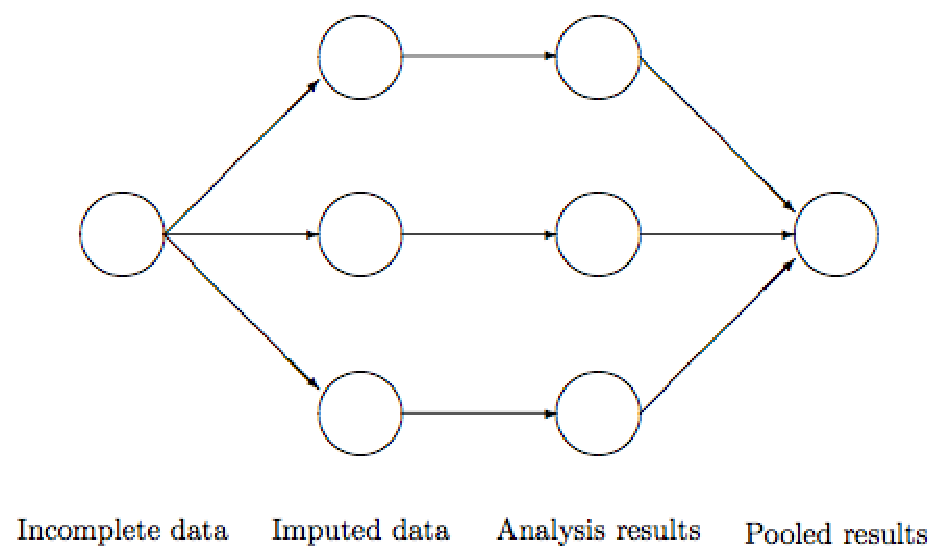
\includegraphics[width=10cm]{Imputacion_muliple_imag1}
\caption{Pasos de la imputación múltiple.}
\label{Fig_imputacion_multiple}
\end{center}
\end{figure}
\begin{itemize}
\newpage
\item[-] \textbf{Paso 1:} Determinar el estimando $Q$.
\item[-] \textbf{Paso 2:} Construir el modelo para obtener $m$ imputaciones para cada valor perdido.
\item[-] \textbf{Paso 3:} Especificar el número $m$ de imputaciones.
\item[-] \textbf{Paso 4:} Asumir $m$ bases de datos completas, una por cada imputación y analizarlas normalmente y guardar los $m$ estimadores y errores estándar que se obtengan.
\item[-] \textbf{Paso 5:} Combinar los estimadores y los errores estándar para obtener un único valor tanto para cada estimador como para su error estándar correspondiente.
\end{itemize}

A continuación vamos a profundizar en cada uno de los pasos, para desarrollar de una manera clara y ordenada la técnica de la imputación múltiple y el porqué de asociarla con el metaanálisis multivariado.

\paragraph{Paso 1:}
El estimando no tiene porqué ser la variable de resultado necesariamente. Cualquier variable con valores perdidos que sea fundamental para construir un modelo estadístico es susceptible de ser escogido como estimando. En este caso no se va a escoger ninguno de los outcomes, que serían nuestras variables de resultado, si no sus correlaciones dentro de cada estudio.

\paragraph{Paso 2:}
La mejor manera de construir el modelo es siguiendo la idea de la estadística bayesiana. El objetivo último es intentar tener una herramienta mediante la que podamos obtener m posibles valores para cada valor perdido. Por otra parte, tenemos que tener en cuenta la incertidumbre acerca del valor que debería tomar en realidad un valor perdido y la mejor manera de tenerla en cuenta es utilizando una distribución de probabilidad.
La mejor distribución para poder extrae de manera aleatoria las imputaciones, es a través de una distribución predictiva y utilizando el \textbf{teorema de Bayes} descrito en \ref{bayes} y más concretamente en \ref{bayes_practica}, podemos construirla. Para ello será necesario establecer la distribución de verosimilitud y la distribución a priori del parámetro de interés (la correlación).
La distribución de verosimilitud es la distribución que tendrá la correlación dados los datos, es decir las observaciones de las parejas de outcomes. La distribución a priori podrá ser informativa, si tenemos evidencias externas suficientes como para suponer que la correlación tomará unos determinados valores o si en cambio, no la tenemos o no la consideramos suficiente, podemos determinarla no informativa dando de esta manera el peso a la distribución de verosimilitud.
En los estudios que se incluirán en es trabajo, podemos encontrarnos en los dos extremos sin ningún término medio. La mejor situación posible sería disponer de los datos individuales ya que podríamos calcular la correlación directamente. Por contra, si no disponemos de ellos únicamente conoceríamos las correlaciones triviales de cada outcome consigo misma y aquí jugaría un papel decisivo la distribución a priori ya que la función de verosimilitud sería totalmente no informativa. En el caso en el que no dispongamos de datos individuales y no podamos especificar una distribución a priori informativa, tendríamos una distribución predicitiva no informativa, en cuyo caso sería $U\left( -1,1\right)$. 

\paragraph{Paso 3:}

Este paso es muy importante ya que del número de imputaciones dependerá la calidad de las inferencias que hagamos y por lo tanto la credibilidad de las conclusiones que extraigamos. Tradicionalmente, el número $m$ de imputaciones recomendado era $m=2,3,4,5$ \cite{Rubin1987}\cite{Rubin1996}\cite{Schafer1997}\cite{Schafer1998}.

Antes de justificar el porqué se recomendaban estos valores $m$, es necesario definir la \textbf{eficiencia relativa} de una variable. La \textbf{eficiencia relativa} es una magnitud que cuantifica la variabilidad de la imputación múltiple respecto a su valor mínimo. Cuya fórmula es la siguiente:
\begin{equation}
RE=\left(1+\frac{\gamma}{m}\right)^{-1} 
\label{eficiencia_relativa}
\end{equation}

Siendo $\gamma$ la proporción de información perdida, que se calcula a partir de la variabilidad tanto total como entre imputaciones de la siguiente manera:
\begin{equation}
\gamma = \frac{V_{B}+\dfrac{V_{B}}{m}}{V_{T}}
\label{gamma}
\end{equation}

La base en la que sustenta la elección de un $m$ tan pequeño es la siguiente. La imputación múltiple es una técnica de simulación, por lo que al calcular $\overline{Q}$ y su varianza $V_{T}$, estamos cometiendo un error de simulación. Haciendo $m=\inf$, se pierde el error de simulación y únicamente tenemos el error atribuible a la variabilidad, es decir $T_{\inf}<T_{m}$ si $m=\inf$. De este modo la pregunta a responder es cuando $T_{\inf}$ está lo sufucientemente próximo a $T_{m}$ para determinar el número de imputaciones. En \cite{VanBuuren2012} se recoge una fórmula que relaciona $T_{\inf}$ con $T_{m}$ a través de la expresión \ref{eficiencia_relativa}:
\begin{equation}
T_{m} = RE \cdot T_{\inf}
\label{det_m_VanBuuren}
\end{equation}

Para entender esta postura basta ver un ejemplo. Supongamos que $\gamma=0.3$ y que hemos hecho $m=5$ imputaciones, de \ref{det_m_VanBuuren} se tiene que $T_{m}=1+\frac{0.5}{5}=1.06$ cuya interpretación es que la varianza obtenida con 5 imputaciones, $T_{5}$, es 1.06 veces la varianza ideal, $T_{\inf}$, dando lugar a un intervalo de confianza un 3\% más largo que el ideal. Siguiendo este razonamiento, si tomamos $m = 15,25$ se tiene que la varianza mejoraría alrededor de un 1\%, por lo que según \cite{Schafer1997} y \cite{Schafer1998} no sería necesario aumentar $m$. En \cite_{Longford} se puede ver cual la relación entre el aumento de $m$ y la disminución de la varianza.

Publicaciones recientes han demostrado que otras características relacionadas con los estimadores no se comportan de la misma manera que $\gamma$ para valores de $m$ pequeños. Graham et al. en \cite{Graham2007} demostraron a través de una simulación como un número pequeño de imputaciones puede tener un efecto nefasto en el poder estadístico, sobre todo dependiendo del valor de $\gamma$. De hecho en la tabla 3 de su publicación vemos como el poder estadístico para el ejemplo anterior es del 73\%, para otras situaciones queda bien claro como el aumentar drásticamente $m$ puede mejorar el poder estadístico, sobre todo cuando $\gamma$ es elevado, con $\gamma=0.90$ el poder es un 50\% superior para $m=100$ que para $m=3$. Además también queda demostrado que $m=20$ como mínimo puede hacer que el poder sea comparables al que se tiene cuando se utiliza máxima verosimilitud.

Royston en \cite{Royston2004} probó cómo los grados de libertad asociados al proceso de imputación múltiple $\nu$ influyen al igual que $m$ en la longitud del intervalo de confianza para $\overline{Q}$ estudiando la inestabilidad del coeficiente de confianza $t_{\nu}\sqrt{V_{T}}$. En esta publicación se ve como los intervalos de confianza para $t_{\nu}\sqrt{V_{T}}$ varían mucho en función de $m$ siendo mucho más estables y estrechos cuanto mayor el número de imputaciones. En \cite{Royston2004} se determina como regla de cálculo de $m$ que sea lo suficientemente grande como para que el coeficiente de variación del parámetro en el peor de los casos sea $<5\%$. Para poder estimar $m$ es suficiente con que $ln(t_{\nu}\sqrt{V_{T}})<0.05$.

Siguiendo esta regla lo que se consigue es que el rango de incertidumbre del intervalo de confianza para $Q$ sea menor del 10\%, fijando $m \geq 20$.

Por su parte Bodner en \cite{Bodner2008} también publicó que un número reducido de imputaciones afecta a magnitudes relacionadas con la inferencia, longitud de intervalos de confianza, p-valores y fracción de información faltante $\lambda$, de una manera muchos más pronunciada que a la eficiencia relativa. A este fenómeno lo definió como varianza de la imputación. Al igual que las publicaciones anteriores, empleó la simulación para ver cual sería el valor de $m$ recomendado. En datos multivariantes, $\lambda$ no es equivalente a la porporción de información perdida \ref{gamma} \cite{Longford2005}, además $\lambda$ en general es desconocida y puede ser estimada mediante \ref{gamma}. La conlusión de esta publicación sigue la línea de \cite{Graham2007} y \cite{Royston2004}, es decir, que para poder obtener unos estimadores cuya inferencia sea estable en el sentido de que aporte unas conclusiones válidas, el  valor de $m$ debe ser mayor que el que tradicionalmente se recomienda. Además gracias a las tablas que se reportan, el $m$ está relacionado con el valor de $\lambda$. En otras palabras, que cuanto mayor sea la presencia de missing values, mayor debe ser el número de imputaciones.

\paragraph{Paso 4:}
Una vez determinadas el número de imputaciones, lo que tenemos es que el estimando $Q$ va a tener $m$ valores, por lo que estaremos trabajando con un vector de longitud $m$. En este paso lo que se hace es asumir que cada una de las componentes de este vector son valores reales. De este modo lo que vamos a tener realmente no es una sola base de datos, sino $m$ de tal forma que en cada una de ellas el valor, perdido será sustituido por la componente correspondiente del vector de $m$ posibles valores.

De este modo hemos pasado de tener una base de datos con valores perdidos a tener $m$ conjuntos completos de datos que se analizarán por separado utilizando la técnica estadística que corresponda \cite{Rubin1978_3}.

\paragraph{Paso 5:}

Una vez analizadas las $m$ bases de datos de forma individual, tenemos $m$ estimadores del mismo parámetro que además son insesgados si los datos son MAR \cite{VanBuuren2012}. Para poder trabajar de una manera cómoda, no podemos estar utilizando los $m$ estimadores constantemente, por lo que se deben combinar de alguna manera. La forma de combinarlos fue introducida por Rubin en \cite{Rubin1987} donde aparecen las fórmulas para el estimador puntual y para la varianza asociada al mismo por el hecho de tener $m$ posibles valores. 

El \textbf{estimador puntual de la imputación múltiple} se define de la siguiente manera:
\begin{equation}
\overline{Q}=\frac{1}{m}\sum_{i=1}^{m}Q_{i}
\label{estimador_puntual_imputacion multiple}
\end{equation}

Es la media muestral de donde $Q_{i}$ es la i-ésima imputación para el valor perdido del parámetro de interés. Es necesario mencionar que no hay ninguna incompatibilidad entre esta definición (frecuentista) y el enfoque bayesiano que emplea Rubin en \cite{Rubin1987} para desarrollar el método de la imputación múltiple. Desde el punto de vista frecuentista, $\overline{Q}$ es el estimador fijo del parámetro poblacional, mientras que desde el punto de vista bayesiano $\overline{Q}$ es la media de la distribución predictiva de la variable aleatoria $Q$  \cite{VanBuuren2012}.

Una vez definido el estimador puntual, nos queda determinar la manera en la que vamos a trabajar con la variabilidad. La variabilidad, bien sea a través de la varianza o del error estándar, se descompone en dos componentes. La primera de ellas es la \textbf{varianza intra-imputaciones}, que es la variabilidad atribuible al hecho de que tenemos $m$ errores estándar, uno por cada $Q_{i}$. La manera de calcularla es a través de:
\begin{equation}
V_{W}=\frac{1}{m}\sum_{i=1}^{m}SE_{i}^{2}
\label{within_var_est_puntual}
\end{equation}

Siendo $SE_{i}$ el error estándar asociado al estimador del parámetro al utilizar la i-ésima imputacion.

La segunda fuente de variabilidad está asociada al hecho de que al tener $m$ bases de datos completas, no encontramos con que realmente calculamos $m$ estimadores del mismo parámetro. Por lo que tenemos que cuantificar la variabilidad relacionada con la variación del estimador del parámetro en las $m$ bases de datos. Esta variabilidad recibe el nombre de \textbf{variabilidad entre imputaciones} y se calcula de la siguiente manera:
\begin{equation}
V_{B}=\frac{1}{m-1}\sum_{i=1}^{m}(\widehat{Q_{i}}-\overline{Q})^{2}
\label{between_var_est_puntual}
\end{equation}

Donde $\widehat{Q_{i}}$ es el estimador del parámetro en la i-ésima base de datos y $\overline{Q}$ es el estimador puntual del parámetro definido en \ref{estimador_puntual_imputacion multiple}.

Siguiendo \ref{within_var_est_puntual} y \ref{between_var_est_puntual}, la variabilidad total se podría definir directamente como la suma de las dos componentes en las que ha sido dividida. Pero se tiene que tener en cuenta una cosa más. En \ref{between_var_est_puntual} estamos introduciendo la cantidad $\overline{Q}$, que es el estimador puntual de la imputación múltiple y como se puede apreciar en \ref{estimador_puntual_imputacion multiple} se ha calculado a partir de una muestra de $m$ valores, por lo que también está sujeto a variabilidad.

Ahora ya sí podemos definir la \textbf{variabilidad total} puesto que ya tenemos en cuenta todas las posibles fuentes de variación. La manera de calcularla es la siguiente:
\begin{equation}
V_{T} = V_{W} + V_{B} + \frac{V_{B}}{m}
\label{total_var_est_puntual}
\end{equation}

Quedando reflejadas:
\begin{itemize}
\item[-] $V_{B}$ la varianza producida por tomar una muestra para representar a toda la población.
\item[-] $V_{W}$ la varianza extra por tener valores perdidos en la base de datos.
\item[-] $\frac{V_{B}}{m}$ la varianza extra de la simulación por ser $\overline{Q}$ una estimación calculada a partir de $m$ observaciones.
\end{itemize}

El objetivo de la imputación múltiple es conseguir un estimador $\widehat{Q}$ del estimando $Q$ que sea \textbf{insesgado} y \textbf{válido en el sentido de confanza} \cite{Rubin1996}. 

Que sea insesgado significa que la media $\widehat{Q}$ de todas las posibles muestras para calcularla sea $Q$, es decir:
\begin{equation}
E(\widehat{Q}\vert Y)= Q
\label{est_insesgado}
\end{equation} 

Mientras que sea válido en el sentido de confianza quiere decir que la media de todos los posibles $V_{W}$, sea mayor o igual qyue la varianza de $\widehat{Q}$, formalmente:
\begin{equation}
E(V_{W}\vert Y)\geq V(Q\vert Y)
\label{validez_confianza}
\end{equation}

Para poder realizar inferencias válidas, es necesario que los valores imputados cumplan unas ciertas características. Las condiciones \ref{est_insesgado} y \ref{validez_confianza} son de necesario cumplimiento para que la estimación del estimando $Q$ sea válida. El objetivo de la imputación múltiple es encontrar un estimador puntual $\overline{Q}$ de $Q$ con propiedades estadísticas adecuadas. Como ya se ha visto, a nivel muestral existe incertidumbre rodeando a $Q$ y está controlada por $V_{W}$. Obviamente si no tuviéramos valores perdidos en la muestra, sería innecesario hacer esto puesto que con $\overline{Q}$ y $V_{W}$ ya tendríamos todo lo necesario.

Cuando se tienen missing values en la muestra, lo que en nuestro caso casi siempre ocurre, debemos distinguir tres niveles de estimación: el de estimación de los missing values, el de estimación con la base de datos completa y por último el nivel poblacional. Todo esto queda muy bien recogido de manera conceptual en la tabla 2.2 de \cite{VanBuuren2012}.

Como ya sabemos, la imputación es el método mediante el que tratamos de completar una base de datos con valores perdidos. Para que esto sea posible, al menos se deben cumplir \ref{est_insesgado} para $\overline{Q}$ y \ref{validez_confianza} para $V_{W}$. Pero para ir un paso más allá y poder decir que el procedimiento de imputación es \textbf{propio en el sentido de confianza}, se deben cumplir las siguientes condiciones:

\begin{itemize}
\item[-] $E(\overline{Q}\vert Y)=\widehat{Q}$. Que el estimador puntual sea un estimador insesgado de $\widehat{Q}$.
\item[-] $E(V_{W}\vert Y)=V_{W}$. El estimador de la varianza intra-imputaciones debe ser insesgado.
\item[-] $(1+\frac{1}{m})E(V_{B}\vert Y)\geq V(\overline{Q})$
\end{itemize}

Si en la tercera condición la desigualdad es estricta se dice que el proceso es \textbf{propio}, aunque es no es necesario para que las inferencias obtenidas sean válidas \cite{VanBuuren2012}
\newpage

\subsection{Creación de las matrices de correlación intra-estudios.}

En esta sección vamos a desarrollar el proceso de imputación de la matriz de correlaciones mediante las reglas de Rubin \ref{within_var_est_puntual} \ref{total_var_est_puntual}.

\subsubsection{Descomposición de la matriz de varianzas-covarianzas.}
Como toda matriz, la matriz de varianzas-covarianzas se puede descomponer de varias formas diferentes (ver pág. 28). El método de descomposión que hemos seleccionado está relacionado con directamente con los datos que se tienen en estos tipos de análisis. Como ya se ha mencionado con anterioridad, en general únicamente se dispone de las desviaciones estándar de los estimadores del efecto de cada una de las variables.

Si se observa la forma de construir una matriz de varianzas-covarianzas vemos que:
\begin{equation}
\Sigma = \left( \begin{array}{cccc}
 \sigma_{1}^{2} &  \rho_{1,2}\sigma_{1}\sigma_{2} & \ldots & \rho_{1,k}\sigma_{1}\sigma_{k}\\
 \rho_{2,1}\sigma_{2}\sigma_{1}  &  \sigma_{2}^{2} & \ldots & \rho_{2,k}\sigma_{2}\sigma_{k}\\
 \vdots & \vdots & \ddots & \vdots\\
 \rho_{k,1}\sigma_{k}\sigma_{1} & \rho_{k,2}\sigma_{k}\sigma_{2} & \ldots & \sigma_{k}^{2}
\end{array} \right)\right) 
\end{equation}

Atendiendo a la regla de multiplicación de matrices, se tiene que en realidad la matriz de varianzas-covarianzas se puede expresar de la siguiente forma:
\begin{equation}
\Sigma =
\left( \begin{array}{cccc}
 \sigma_{1} &  0 & \ldots & 0 \\
 0  &  \sigma_{2} & \ldots & 0 \\
 \vdots & \vdots & \ddots & \vdots\\
 0 & 0 & \ldots & \sigma_{k}}
\end{array} \right)\right)
\left( \begin{array}{cccc}
1 &  \rho_{1,2} & \ldots & \rho_{1,k}\\
 \rho_{2,1}  &  1 & \ldots & \rho_{2,k}\\
 \vdots & \vdots & \ddots & \vdots\\
 \rho_{k,1} & \rho_{k,2} & \ldots & 1
\end{array} \right)\right)
\left( \begin{array}{cccc}
 \sigma_{1} &  0 & \ldots & 0 \\
 0  &  \sigma_{2} & \ldots & 0 \\
 \vdots & \vdots & \ddots & \vdots\\
 0 & 0 & \ldots & \sigma_{k}}
\end{array} \right)\right)
\label{descomposicion_sigma}
\end{equation}

Es decir, la matriz de varianzas-covarianzas se puede descomponer como un producto de tres matrices, dos matrices diagonales con las desviaciones estándar de los estimadores del efecto y una matriz con los coeficientes de correlación de las variables de resultado \cite{Barnard2000}. De esta manera los únicos parámetros que desconocemos son los de la matriz central y serán los que estimaremos.

\subsubsection{Construcción de la matriz de correlación.}
Tras seleccionar la descomposición \ref{descomposicion_sigma}, el problema de la construcción de las matrices de varianzas-covarianzas se ha transformado en la estimación de la matriz de correlaciones. Con lo cual, la estrategia a seguir para resolver este problema será establecer el mejor método de estimación de la matriz de correlaciones.

Antes de comenzar a detallar la estrategia, es necesario enumerar tres características que van a ser muy importantes a la hora de entender y explicar de una forma ordenada la técnica de estimación de la matriz de correlaciones.

\begin{itemize}
\item[-] Es una matriz simétrica con 1 en la diagonal principal.
\item[-] Los elementos que están fuera de la diagonal principal, están comprendidos en el intervalo $[-1,1]$.
\item[-] Es una matriz semidefinida positiva, es decir, $\mathbf{det}(\mathbf{R})\geq 0$. 
\end{itemize}

La primera de las tres características nos dice cuántos elementos vamos a tener que estimar, el cual depende obviamente del número de variables de resultado que tengamos en los estudios y la relación entre el número de variables y el de coeficientes de correlación no es lineal, lo que se traduce en problemas cuando tenemos muchas variables de resultado entre manos.
En general dados $k$ estimadores del efecto, el número de coeficientes de correlación que tendremos que estimar será: $$(\dfrac{k(k+1)}{2})-k$$

La segunda de las características establece qué tipo de distribuciones de probabilidad podemos utilizar para estimar los diferentes coeficientes. En el estudio de \cite{Barnard2000} se realiza estableciendo distribuciones multivariantes como es la distribución uniforme conjunta, ya que como todos los coeficientes de correlación están definidos en el mismo intervalo, de esta manera se estiman simultáneamente. 

En este trabajo de investigación se va a proponer una estrategia alternativa, como cuando se está investigando un tema para más tarde realizar una revisión sistemática, se maneja más información de la que realmente se va a necesitar en relación a la posible relación existente entre las diferentes variables de resultado. Si esta información extra, o incluso las propias sospechas del investigador pudieran utilizarse de algún modo, estaríamos entrando en el campo de la estadística bayesiana lo que podría beneficiar a nuestros análisis.

Siguiendo con lo mencionado anteriormente, aunque sabemos exactamente el rango de valores entre los que se mueven los coeficientes de correlación, en realidad no tiene porqué distribuirse de la misma manera. Esta es la idea en la que se apoya la técnica que aquí se va a plantear, especificar la distribución de probabilidad de cada coeficiente de correlación por separado. De esta manera podemos hacer una aproximación a la estimación de estos coeficientes de una manera mucho más general.

En las situaciones en las que podamos asumir que el coeficiente correspondiente va a ser mayor que cero, lo que se traduce en una correlación directa de las variables, podemos utilizar la distribución beta que gracias a sus dos parámetros hace que sea muy flexible, los cuales se pueden determinar utilizando R, lo que es muy positivo para nuestros intereses. Por otro lado podemos utilizar también distribuciones continuas y truncarlas en un determinado intervalo donde creemos que se va a encontrar el verdadero valor del coeficiente de correlación, en esta situación podríamos emplear la por ejemplo la distribución normal ya que en R se puede truncar entre cualesquiera dos valores y también se pueden fijar sus parámetros dando dos cuantiles y sus correspondientes probabilidades. En cambio si nos encontrásemos en el peor de los escenarios posibles, es decir, cuando no sepamos nada acerca del o de los coeficientes, siempre podríamos utilizar la distribución uniforme, siguiendo lo publicado en \cite{Barnard2000}.

Por último hemos de hablar de que una matriz de correlaciones es semidefinida positiva. Aunque no lo parezca, esta condición es la más restrictiva de todas con muchísima diferencia. Para entender esto mejor hemos de comprender el trabajo de \cite{Rousseeuw1994}. Establece una aplicación que asocia a cada matriz con un vector construido con los coeficientes de correlación y acto seguido se aplica la condición de que $\mathbf{det}(\mathbf{R})\geq 0$ para que sea de correlación. Como dentro de la superficie el $\mathbf{det}(\mathbf{R})> 0$ y fuera $\mathbf{det}(\mathbf{R})< 0$, la superficie determina un cuerpo sólido.

El estudio del volumen de este cuerpo es la herramienta necesaria para saber cuál es la cantidad de matrices de correlación que existen en relación con todas las matrices definidas en el intervalo $[-1,1]^{k}$. A continuación vamos a entrar de lleno en el porqué del carácter restrictivo de la tercera de las condiciones. Para ello vamos a ver la evolución de la condición cuando vamos aumentando el número de variables de resultado:

Cuando tenemos \textbf{dos variables}, el conjunto de puntos que representan a todas las matrices de correlación es el siguiente $$C=\lbrace r_{XY}\in \mathbb{R} \vert -1\leq r_{XY} \leq 1, 1-r_{XY}^{2} \geq 0\rbrace$$ siguiendo la idea de \cite{Rousseeuw1994}, vamos a representar el conjunto \textbf{C} dentro del conjunto de todas las matrices $\mathcal{M}_{2\times  2}[-1,1]$:
\newpage
\medskip 
\begin{figure}[htb]
\begin{center}
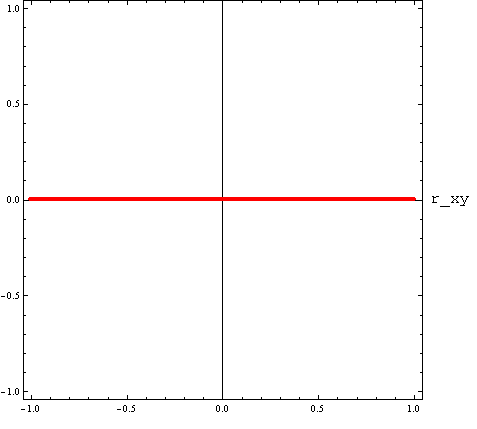
\includegraphics[width=10cm]{matriz_correlacion_2vars}
\caption{Representación gráfica del conjunto de las matrices de correlación de dos variables.}
\label{Fig_matriz_correlacion_2vars}
\end{center}
\end{figure}

Como se puede apreciar, coincide con $\mathcal{M}_{2\times  2}[-1,1]$. Por tanto si dividimos la longitud de $C$ entre la longitud de $[-1,1]$, tenemos que: $$\dfrac{\mathbf{Long}(C)}{\mathbf{Long}([-1,1])}=\dfrac{1}{1}=1$$
Lo que quiere decir que cualquier matriz $\mathbf{M}\in \mathcal{M}_{2\times  2}[-1,1]$ es una matriz de correlación para alguna pareja de variables, argumento que se deduce de manera trivial puesto que $1-r_{XY}^{2} \geq 0$ siempre se cumple con este tipo de matrices.

{\normalsize Cuando tenemos \textbf{tres variables}, el número de coeficientes de correlación diferentes pasa a ser 3 y que la fórmula del determinante de una matriz de correlaciones es 
$\mathbf{det(C)}=1+2r_{XY}r_{XZ}r_{YZ}-r_{XY}^{2}-r_{XZ}^{2}-r_{YZ}^{2}$. De este modo el conjunto de matrices de correlación de tres variables es} {\tiny $$C=\lbrace\lbrace r_{XY},r_{XZ},r_{YZ}\rbrace \in \mathbb{R}^{3} \vert \lbrace r_{XY},r_{XZ},r_{YZ} \rbrace \in [-1,1]^{3}, r_{XY}^{2}+r_{XZ}^{2}+r_{YZ}^{2}-2r_{XY}r_{XZ}r_{YZ} \geq 1 \rbrace$$}
Si representamos el conjunto $C$ dentro de $[-1,1]$ obtenemos la siguiente figura:
\newpage
\medskip 
\begin{figure}[htb]
\begin{center}
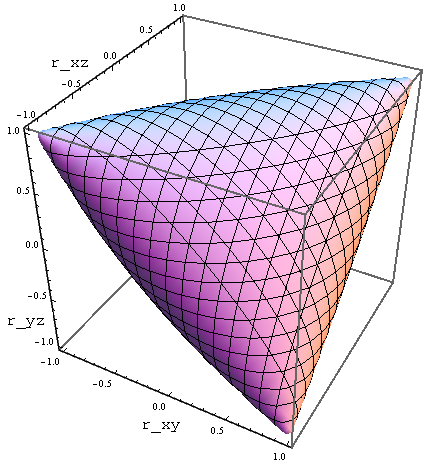
\includegraphics[width=10cm]{matriz_correlacion_3vars}
\caption{Representación gráfica del conjunto de las matrices de correlación de tres variables.}
\label{Fig_matriz_correlacion_2vars}
\end{center}
\end{figure}

Como se puede apreciar, $C\subset [-1,1]^{3}$ por lo que ya no todas las matrices representadas en $[-1,1]^{3}$ son matrices de correlación. Por tanto es muy interesante saber exactamente cual es la proporción de matrices de correlación que existen en relación a la totalidad de matrices representadas en el cubo. Para saberlo vamos a seguir con la idea del caso en el que teníamos dos variables, es decir, vamos a dividir el volumen de $C$ entre el volumen de $[-1,1]$: $$\dfrac{\mathbf{Vol}(C)}{\mathbf{Vol}([-1,1]^{3})}=\dfrac{\frac{\pi^{2}}{2}}{2^{3}}=\dfrac{\pi^{2}}{8}\approx 0.617$$
Una vez hecho el cálculo se tiene que el volumen de $C$ representa el 61.7\% del volumen del cubo, en otras palabras, dada una matriz simétrica, con 1 en su diagonal principal y con el resto de elementos comprendidos en el intervalo $[-1,1]$, la probabilidad de que sea de correlación es del 61.7\%. 

La situación ya es mucho más complicada cuando se trabaja con \textbf{cuatro variables}. El número de coeficientes de correlación diferentes en este escenario es de 6, por lo que ya no podemos representar gráficamente nada debido a que vamos a trabajar en $\mathbb{R}^6$. Además el determinante de una matriz perteneciente a $\mathcal{M}_{6\times  6}[-1,1]$ es un polinomo de grado 4, con lo que los cálculos también se complican. De este modo el conjunto de las matrices de correlación para cuatro variables es el siguiente:

La situación se vuelve mucho más complicada cuando pasamos a tener \textbf{más de cuatro variables}. Aunque las propiedades del conjunto $C$ se siguen heredando, tanto el número de coeficientes de correlación como el grado de $\mathbf{det}(M)$ crecen de manera no lineal, para hacernos un idea en el caso de cuatro variables tenemos 6 coeficientes de correlación y el grado del determinante es 4. En general y hablando sólo del número de coeficientes de correlación, si tuviésemos $n$ variables, sería de $\dfrac{n(n-1)}{2}-n$ con lo que el grado de su determinante sería muy elevado.

Por otra parte, seria imposible representar representar gráficamente el conjunto $C$, ya que en el caso de cuatro variables, sería un subespacio de $\mathbb{R}^6$ y en el caso general le sería de $\mathbb{R}^{\frac{n(n-1)}{2}}$. Para poder calcular analíticamente el volumen de $C$ sea cual sea el número de variables, hemos de utilizar las fórmulas publicadas en \cite{Joe2005} y \cite{Hurliman2012}, siendo la más manejable y sencilla la de \cite{Hurliman2012}:
\begin{equation}
\mathbf{V_{n}}=\mathbf{Vol}(C_{n})=\prod_{k=1}^{n-1}(J_{k}^{k}), J_{k}=\int_{-1}^{1}(1-t^{2})^{\frac{1}{2}(k-1)}dt
\label{vol_C}
\end{equation}

Siguiendo el método para calcular la probabilidad de obtener matrices de correlación explicado en el caso de dos y tres variables, se puede determinar, utilizando \ref{vol_C}, una fórmula para calcular dicha probabilidad en el caso de $n$ variables:
\begin{equation}
\mathbf{Prob_{n}}=\dfrac{\mathbf{Vol}([-1,1]^{n})}{\mathbf{Vol}(C_{n})}=\dfrac{2^{n}}{\prod_{k=1}^{n-1}(J_{k}^{k})}
\label{prob_matriz_corr}
\end{equation}

De este modo a partir de \ref{prob_matriz_corr}, se obtiene la siguiente tabla de probabilidades de obtención de matrices de correlación según el número de variables:
\newpage
\begin{table}[!hbt]
\begin{center}
\begin{tabular}{|c|c|}\hline
Variables & Probabilidad  \\\hline
4 & 0.1827705  \\
5 & 0.02200445  \\
6 & 9.495203\times 10^{-4}  \\
7 & 1.328384\times 10^{-5}  \\
8 & 5.542263\times 10^{-8}  \\
9 & 6.419641\times 10^{-11} \\
10 & 1.939125\times 10^{-14} \\
\hline
\end{tabular}
\caption{Probabilidad de obtener una matriz de correlación en función del número de variables.}
\end{center}
\end{table}

Recapitulando lo visto hasta el momento, tenemos que el problema de estimar las matrices de varianzas-covarianzas se ha reducido al cálculo de las matrices de correlación. Por otra parte, hemos de añadir la cuestión de que cualquier matriz únicamente por ser: simétrica, con 1 en la diagonal principal y con el resto de elementos en $[-1,1]$ no tiene porqué ser de correlación. Esto último se traduce en que cada matriz de esas características que se obtenga durante el proceso de imputación debe ser comprobada, es decir, debe tener el determinante no negativo.

Este nuevo problema nos plantea la siguiente disyuntiva una vez establecido el número de imputaciones a realizar:
\begin{itemize}
\item[-] Estimar una cantidad ingente de matrices para que por azar cubramos el número de imputaciones. 
\item[-] Obtener tantas matrices como imputaciones y transformar aquellas que no cumplan las tres condiciones.
\end{itemize}

De estas dos posibles soluciones la segunda solución es la más sensata, ya que existen en la literatura multitud de técnicas que permiten dada una matriz no semidefinida positiva, transformarla en la que sí lo sea y además que sea lo más similar posible.

\subsubsection{Fundamentos teóricos de los métodos de transformación de matrices no semidefinidas positivas.}
Este punto es el más importante de todo el proceso de imputación, ya que si utilizamos en el proceso de imputación las matrices de correlación matrices que no lo son, no sólo estamos sesgando la credibilidad del proceso, sino que estamos yendo en contra del propio modelo del metaanálisis multivariado. Si recordamos la formulación del modelo, \ref{re_multi_marginal}, estamos asumiendo que para cada estudio existe una distribución normal multivariante que es seguida por las variables de resultado. Pues bien, si nosotros utilizamos una matriz que no es semidefinida positiva para imputar la matriz de varianzas-covarianzas, lo que realmente estamos haciendo es asumir que los outcomes siguen una distribución de probabilidad que no existe, lo que llevaría al traste todo nuestro modelo.

Por lo tanto tenemos que asegurarnos bien de que esta propiedad se cumple y en el caso de detectar que no en cualquiera de las matrices que se obtengan para la imputación, tratar de transformarlas para que si la cumplan. Además lo que se pretende con la transformación no sólo hacer que la matriz en cuestión cumpla con la última de las propiedades sino que además la matriz que se obtiene sea lo más parecida posible a la matriz de partida.

Antes de empezar a hablar de los métodos de transformación de matrices, es necesario definir los conceptos de similaridad de dos matrices y los conjuntos de matrices simétricas y de matrices de correlación.

Vamos a definir el \textbf{conjunto de matrices simétricas reales de orden $n$ y semidefinidas positivas} como:
\begin{equation}
S_{n}=\lbrace \mathbf{A}\in \mathcal{M}_{n\times n}(\mathbb{R}) \vert \mathbf{A}=\mathbb{A^{t}}, \mathbb{A}\geq 0\rbrace
\label{S_n}
\end{equation}
De forma similar vamos a determinar el \textbf{conjunto de matrices reales cuadradas de orden $n$ con 1 en la diagonal principal} como: 
\begin{equation}
U_{n}=\lbrace \mathbf{A}\in \mathcal{M}_{n\times n}(\mathbb{R}) \vert a_{ii}=1, \forall i \in \lbrace 1,\ldots n\rbrace \rbrace
\label{U_n}
\end{equation}

Para poder determinar si una matriz es similar a otra dada, necesitamos utilizar alguna herramienta que nos de una idea de la proximidad entre ambas. El conjunto sobre el que estamos trabajando es $\mathcal{M}_{n\times n}(\mathbb{R})\equiv \mathbb{R}^{n\times n}$ que es un espacio vectorial, por tanto podemos definir la siguiente función:
\begin{equation}
\begin{array}{cccc}
\vert\vert \cdot \vert\vert_{F}: & \mathcal{M}_{n\times n}(\mathbb{R}) & \longrightarrow & \left[0,\infty\right)   \\
 & \mathbf{A} & \mapsto & \vert\vert \mathbf{A} \vert\vert_{F} =\sqrt{\mathbf{tr}(\mathbf{A}^{t}\mathbf{A})}
\end{array}
\label{norma_frob}
\end{equation}
que recibe el nombre de \textbf{norma de Fröbenius} y satisface las siguientes propiedades:
\begin{itemize}
\item[i)] $\vert\vert \mathbf{A}\vert\vert_{F} \geq 0, \forall \mathbf{A}\in \mathcal{M}_{n\times n}(\mathbb{R})$
\item[ii)] $\vert\vert \mathbf{A}\vert\vert_{F} = 0 \Leftrightarrow \mathbf{A}=0$
\item[iii)] $\vert\vert \alpha\mathbf{A}\vert\vert_{F}=\vert\alpha\vert \vert\vert \mathbf{A}\vert\vert_{F}, \forall \alpha \in \mathbb{R}$ y $\forall \mathbf{A}\in \mathcal{M}_{n\times n}(\mathbb{R})$
\item[iv)] $\vert\vert \mathbf{A}\mathbf{B}\vert\vert_{F} \leq \vert\vert \mathbf{A}\vert\vert_{F}\vert\vert \mathbf{B}\vert\vert_{F}, \forall \mathbf{A},\mathbf{B} \in \mathcal{M}_{n\times n}(\mathbb{R})$
\end{itemize}

Utilizando la norma de Fröbenius, tenemos que $(\mathcal{M}_{n\times n}(\mathbb{R}),\vert\vert.\vert\vert_{F})$ es un espacio normado y como tal sobre él podemos definir una distancia $d(x,y)=\vert\vert(x-y)\vert\vert$ que hace que $(\mathcal{M}_{n\times n}(\mathbb{R}),d)$ sea un espacio métrico y por lo tanto topológico cuya distancia es $d(\mathbf{X},\mathbf{Y})_{F}=\vert\vert \mathbf{X}-\mathbf{Y}\vert\vert_{F}=\sqrt{tr((\mathbf{X-Y}^{t})(\mathbf{X-Y})}$

Una vez construido el espacio métrico $(\mathcal{M}_{n\times n}(\mathbb{R}),d_{F})$ y los conjuntos definidos en \ref{S_n} y \ref{U_n}, estamos en condiciones de determinar formalmente el objetivo de los diferentes métodos de transformación que vamos a describir a continuación. Como lo que pretendemos es encontrar una matriz $\mathbf{X}$ que cumpla con todos los requisitos de las matrices de correlación y que sea lo más próxima a una dada que no sea semidefinida positiva, lo que se persigue es:
\begin{equation}
\gamma(\mathbf{A})=\min_{\mathbf{X} \in S_{n} \cap U_{n}}\lbrace\vert\vert \mathbf{A}-\mathbf{X} \vert\vert_{F}\rbrace
\label{min_dist_frob}
\end{equation}

\subsubsection{Métodos de transformación para obtener matrices de correlación.}

La obtención de matrices de correlación a partir de matrices de pseudo-correlación, es un problema que ha trascendido más allá del metaanálisis multivariado. De hecho, la utilización de matrices de correlación es muy importante dentro del ámbito de las finanzas, manejo de riesgos, análisis de stock, álgebra e incluso en la validación de métodos de análisis estadístico. En definitiva, en campos en los que la relación entre las variables que se manejan son tan importantes como las propias variables.

En consecuencia es abundante la presencia de diferentes algoritmos en la literatura. Aquí vamos a hablar de los diferentes algoritmos encontrados por orden de publicación. Estos serán los que se aplicarán a los datos extraídos de la revisión sistemática y nos quedaremos con aquél que estime las matrices de correlación más próximas, en términos de la distancia de Fröbenius \ref{norma_frob}.

\textbf{\underline{1. Ronald L. Iman \& James.M. Davenport (1982):}}

Este algoritmo publicado en \cite{Iman1982}, se basa en una pequeña modificación de los valores propios de la matriz a transformar. La modificación del espectro de la matriz es pequeña porque si el cambio en los valores propios son leves, lo mismo ocurrirá en los elementos de la matriz, que es justamente lo que pretendemos.

El algoritmo en cuestión consta de dos pasos y una manipulación previa de la matriz.

\textbf{Paso previo:} Sea $\mathbf{C} \in \mathcal{M}_{n\times n}(\mathbb{R})$ de pseudo-correlación, por tener sus elementos reales es una matriz diagonalizable. Es decir, existen dos matrices $\mathbf{Z}$ y $\mathbf{D}$ tales que $\mathbf{C}=\mathbf{Z}\mathbf{D}\mathbf{Z^{t}}$ siendo $\mathbf{D}$ diagonal cuya diagonal principal está formada por los valores propios de $\mathbf{C}$ (reales también) y las columnas de $\mathbf{Z}$ son los vectores propios asociados.

Sean $\lambda_{1}<\lambda_{2}<\ldots<\lambda_{n}$ los elementos de $\mathbf{D}$ ordenados de menor a mayor y supongamos que los primeros $k$ son negativos.

\textbf{Paso 1:} Cambiar cada uno de los $\lambda_{i}, i \in \lbrace 1,\ldots,k\rbrace$ por una cantidad positiva $\epsilon$. Esta cantidad se debe escoger muy pequeña para alterar lo mínimo posible la matriz original $\mathbf{C}$ y convertirla en definida positiva.

\textbf{Paso 2:} Examinar la magnitud del resto de valores propios, $\lambda_{i}, i \in \lbrace k+1,\ldots,n\rbrace$, y cambiar sus valores de acuerdo a la siguiente norma:

$$\lambda_{i}^{*}=\left\lbrace
  \begin{array}{l}
     $\epsilon$ si $\lambda_{i}\leq \epsilon$ \\
     $\lambda_{i}$ si $\lambda_{i} > \epsilon$ \\
  \end{array}
  \right.$$

consiguiendo mejorar las características operativas del algoritmo.

Tras estos dos pasos calculamos la matriz:
\begin{equation}
\mathbf{C^{*}}=\mathbf{Z}\mathbf{D^{*}}\mathbf{Z^{t}}
\label{est_mat_corr_alg1}
\end{equation}

En general deberemos de escalar los elementos de $\mathbf{diag}(\mathbf{C^{*}})$ sean 1 (véase a continuación). Los elementos de fuera de la diagonal no deben ser retocados porque cuando el algoritmo converge siempre que se tiene que $r_{ij} \in [-1,1]$.

En el caso de que la matriz $\mathbf{C^{*}}$ sea definida positiva el algoritmo se termina, pero si esto no se cumple se toma $\mathbf{C^{*}}$ como $\mathbf{C}$ y se aplican los dos pasos, hasta que en alguna iteración el algoritmo finalmente converja.

Como se ha mencionado anteriormente, existen diferentes maneras de realizar el ajuste de la matriz $\mathbf{C^{*}}$:
\begin{itemize}
\item[-]\textbf{Método A:} Sustituir los elementos de la diagonal por 1. 
\item[-]\textbf{Método B:} Igualar a 1 los elementos de la diagonal principal y en caso de que por motivos de redondeo, algún elemento de fuera de la diagonal no esté en $[-1,1]$, sustituirlo por $-0.999$ ó $0.999$ según corresponda. 
\item[-]\textbf{Método C:} Cada elemento de una fila se divide por la raíz cuadrada del elemento de dicha fila que esté en la diagonal. Se procede de la misma manera con los elementos de cada columna: $$r_{i,j}^{*}=\dfrac{r_{ij}}{\sqrt{r_{ii}r_{jj}}}$$
\item[-]\textbf{Método D:} Aplicar el método anterior solamente en aquellos elementos que no están en el rango $[-1,1]$.
\item[-]\textbf{Método E:} Muy similar al método anterior pero la fórmula tiene la siguiente modificación: $$r_{ij}^{*}=\dfrac{r_{ij}}{\sqrt{(r_{ii}-0.05)(r_{jj}-0.05)}}$$
\end{itemize}

En los métodos C, D, y E los elementos de la diagonal principal de la matriz son 1.

De acuerdo a la publicación, el método que vamos a emplear en la transformación va a ser el \textbf{método A}, ya que es el que mejor prestaciones ofrece.

\textbf{\underline{2. Peter J. Rousseeuw \& Geert Molenberghs (1993):}}

Estos autores desarrollan en su publicación \cite{Rousseeuw1993} varias técnicas de transformación de matrices, que dividen en dos categorías \textbf{métodos de contracción (lineal y no lineal} y \textbf{métodos de no contracción}.

El método de contracción lineal, calcula los valores propios de la matriz $\mathbf{C}$ y calcula la matriz de correlación de la siguiente manera:
\begin{equation}
\mathbf{\widehat{C}}=\lambda\mathbf{C}+(1-\lambda)\mathbf{I_{n}}
\label{est_mat_corr_alg2}
\end{equation}

Siendo $\lambda$ el mayor valore propio en el intervalo $[0,1]$ que haga a \ref{est_mat_corr_alg2} semidefinida positiva. 

La técnica no lineal se centra en actuar sobre cada elemento que no está en la $\mathbf{diag(C)}$ transformándolo mediante una función no lineal $f: [-\infty,\infty] \longrightarrow [-1,1]$ continua y monótona creciente. La transformación se realiza de la siguiente manera:
\begin{equation}
\widehat{c}_{ij}=\left\lbrace
  \begin{array}{l}
     $f^{-1}(f(c_{ij})+\Delta)$ si $c_{ij}<-f^{-1}(\Delta)$ \\
     $0$ si $\vert r \vert \leq f^{-1}(\Delta)$ \\
     $f^{-1}(f(c_{ij})-\Delta)$ si $c_{ij}>f^{-1}(\Delta)$ \\
  \end{array}
  \right.
\label{est_mat_corr_alg3}
\end{equation} 

siendo $\Delta$ un número positivo próximo a cero, repitiendo \ref{est_mat_corr_alg3} hasta que $\mathbf{\widehat{C}}$ fuera semidefinida positiva. Las siguientes funciones son muy utilizadas:
\begin{itemize}
\item[-] $f_{1}(x)=\dfrac{e^{x}-e^{-x}}{e^{x}+e^{-x}}=\tanh(x)$ y $f^_{1}{-1}(x)=\dfrac{1}{2}\ln(\dfrac{1+x}{1-x})=\tanh^{-1}(x)$
\item[-] $f_{2}(x)=\dfrac{2}{\pi}\arctan(x)$ y $f_{2}^{-1}(x)=\tan(x \dfrac{\pi}{2})$
\end{itemize}

En cuanto a los métodos de no contracción, el primero del que habla es el \textbf{método del valor propio} y es muy similar al mencionado en \cite{Iman1982}, utilizando una variante del metodo C para ajustar la matriz y que sea de correlación. Los pasos del algoritmo son los siguientes:

\textbf{Paso 1:} Encontrar una matriz diagonal $\mathbf{D}$ y una matriz ortogonal $\mathbf{P}$ de tal manera que: $$\mathbf{C}=\mathbf{P}\mathbf{D}\mathbf{P^{t}}$$ donde $\mathbf{diag(D)=\lbrace \lambda_{1},\ldots,\lamda_{n}\rbrace}$ los valores propios de $\mathbf{C}$ y las filas de $\mathbf{P}$ formadas por los vectores asociados a dichos valores propios.

\textbf{Paso 2:} En el caso de que $\mathbf{C}$ no sea ni semidefinida positiva ni definida positiva, al menos uno de los $\lambda_{i}, i=1,\ldots,n$ será negativo por lo que tendremos que hacer:
$$\lambda_{i}^{*}=\left\lbrace
  \begin{array}{l}
     $\epsilon$ si $\lambda_{i}\leq 0$ \\
     $\lambda_{i}$ si $\lambda_{i} > 0$ \\
  \end{array}
  \right.$$
en le caso en el que precisemos de una matriz definida positiva, si lo que queremos es que simplemente lo sea semidefinida, basta con hacer $\epsilon=0$. Una vez hecho esto, se sustituye la matriz $\mathbf{D}$ por $\mathbf{D'}$.

\textbf{Paso 3:} Construimos la matriz $\mathbf{C'}=\mathbf{P}\mathbf{D'}\mathbf{P^{t}}$, pero como en general la diagonal de $\mathbf{C'}$ no tiene porqué estar compuesta de 1, tenemos que ajustarla. Para ello generamos una matriz diagonal $\mathbf{D_{1}}$ con $\frac{1}{\sqrt{c_{jj}^{'}}}, j=1,\ldots,n$, y finalmente se construye la matriz de correlación que buscamos de la siguiente manera:
\begin{equation}
\mathbf{\widehat{C}}=\mathbf{D_{1}}\mathbf{C'}\mathbf{D_{1}}
\label{mat_corr_alg4}
\end{equation}

El segundo método recibe el nombre de \textbf{método de escalado}. Enfoca el problema de encontrar la matriz de correlaciones más próxima a una dada como un problema de optimización. Trata de encontrar la mejor matriz de correlaciones mediante la minimización de un criterio que refleje la proximidad entre dos matrices. En \cite{Rousseeuw1993} se mencionan dos posibles funciones:
\begin{equation}
S=\sum_{i=1}^{n}\sum_{j=1}^{n}(c_{ij}-c_{ij}^{'})^{2}
\label{dist_euclidea}
\end{equation}
\begin{equation}
S_{w}=\sum_{i=1}^{n}\sum_{j=1}^{n}w_{ij}(c_{ij}-c_{ij}^{'})^{2}
\label{dist_euclidea_pond}
\end{equation}

La función definida en \ref{dist_euclidea}, está relacionada con el método estadístico de escalado multidimensional y es una potencia de la distancia euclídea. En cambio, \ref{dist_euclidea_pond} asume que la confianza entre los coeficientes de correlación no es la misma. Confianza que se puede cuantificar mediante el parámetro $w_{ij}$.

De este modo este algoritmo se centra en buscar una matriz $\mathbf{\widehat{C}}$ en la intersección de los conjuntos definidos en \ref{U_n} y \ref{S_n} que haga mínima \ref{dist_euclidea} o \ref{dist_euclidea_pond}. Como $U_{n}\cap S_{n} \in \mathbb{R}^{n\times n}$ y además es compacto y convexo la matriz que buscamos existe y además es única \cite{Rousseeuw1993} \cite{Higham2002}. 

La forma de encontrar $\mathbf{\widehat{C}}$ tiene que ser geométrica ya que desde el punto de vista computacional es inabarcable \cite{Rousseeuw1993}. Podemos asumir que los coeficientes de correlación $\widehat{r_{ij}}$ tienen varianza 1 por lo tanto cada una de ellos se puede representar como el producto de dos vectores unitarion de $\mathbb{R}^{n}$, $\widehat{r_{ij}}=U_{i}^{t}U_{j}$. Extendiendo esta idea podemos construir la propia matriz $\mathbf{\widehat{C}}$ como $\mathbf{\widehat{C}}=\mathbf{U^{t}\mathbf{U}}$ estando $\mathbf{U}$ formada por los diferentes vectores columna $U_{i}$.

Basándonos en el hecho de que $\mathbf{\widehat{C}}\in S_{n}$ se deduce del teorema de Choleski para la descomposición de matrices que la matriz $\mathbf{U}$ es una matriz triangular superior con elementos no negativos en la diagonal principal. De este modo, la columna $U_{i}$ solo va a tener $i-1$ componentes libres y además $\vert\vertU_{i}\vert\vert^{2}=1$.

Una buena manera de representar los elementos de $\mathbf{U}$ es mediante funciones goniométricas y haciendo que los $u_{ij}$ sean ángulos, es decir, $U_{i}=(\theta_{1i},\theta_{2i},\ldots,\theta_{(i-1)i})^{t}, i=1,\ldots,n$. Una vez construida la matriz, podemos recuperar $\mathbf{U}$ mediante:
$$u_{ji}=\left\lbrace
  \begin{array}{l}
     $\sin(\theta_{i1})\sin(\theta_{i2})\ldots\sin(\theta_{i,i-j})\cos(\theta_{i,i-j+1})$ si $j \leq i$ \\
     $0$ si $j>i$ \\
  \end{array}
  \right.$$

Una vez planteado el problema de esta manera, se dan las condiciones necesarias para que se puedan aplicar algoritmos numéricos que se encarguen de encontrar los $\theta_{ij}$ adecuados para minimizar cualquiera de las expresiones definidas en \ref{dist_euclidea} y \ref{dist_euclidea_pond}.

Los autores de \cite{Rousseeuw1993}, finalizan diciendo que los dos últimos métodos son superiores a los métodos de contracción. La razón es porque actúan sobre toda la matriz de forma conjunta, no como los mencionados métodos de contracción que lo hacen sobre cada elemento de la matriz individualmente, por lo que los $\widehat{c_{ij}}$ no decrecen tanto. Por otra parte son más fáciles de aplicar y demandan menos capacidad de computación.

\textbf{\underline{3. Ricciardo Rebonato \& Peter Jäckel (1999):}}

El trabajo publicado en \cite{Rebonato2000} está enfocado en la rama de las finanzas, pero los algoritmos que presenta pueden ser perfectamente aplicables en nuestro contexto. 

El primero de ellos recibe el nombre de \textbf{descomposición espectral} y se sustenta en el mismo teorema que el recogido en \cite{Iman1982}. Parte de la expresión $\mathbf{C}\mathbf{S}=\mathbf{D}\mathbf{S}$ donde $\mathbf{D}$ es una matriz diagonal compuesta por los valores propios de $\mathbf{C}$ y la matriz $\mathbf{S}$ es una matriz ortogonal cuyas columnas son los vectores propios asociados a cada uno de los $\lambda_{i}$. 

Las diferencias entre éste algoritmo y el anterior están en la manera de manipular la matriz $\mathbf{D}$ y en la manera de ajustar la matriz resultante para que sea de correlación. Los pasos a dar si se sigue este algoritmo son los siguientes:

\textbf{Paso 1:} Calcular las matrices $\mathbf{D}$ y $\mathbf{S}$ tales que se cumpla: $$\mathbf{C}\mathbf{S}=\mathbf{D}\mathbf{S}$$

\textbf{Paso 2:} Definir a partir de los $\lambda_{i}$ de $\mathbf{D}$, los elementos de $\mathbf{D}'$ según la siguiente norma: 
$$\lambda_{i}^{'}=\left\lbrace
  \begin{array}{l}
     $\lambda_{i}$ si $\lambda_{i}\geq 0$ \\
     $0$ si $\lambda_{i} < 0$ \\
  \end{array}
  \right.$$

\textbf{Paso 3:} Se construyen las matrices $\mathbf{T}$,$\mathbf{B}$ y $\mathbf{B'}$ para realizar los ajustes necesarios y que la matriz resultante sea de correlación de la siguiente manera: 
$$\mathbf{T}: t_{i}[\sum_{m}=s_{im}^{2}\lambda_{m}^{'}]^{-1}$$
$$\mathbf{B'}=\mathbf{S\sqrt{\mathbf{D'}}}$$
$$\mathbf{B}=\sqrt{\mathbf{T}}\mathbf{B'}=\sqrt{\mathbf{T}}\mathbf{S}\sqrt{\mathbf{D'}}$$

\textbf{Paso 4:} Se calcula la matriz $\mathbf{\widehat{C}}$ mediante la expresión:
\begin{equation}
\mathbf{\widehat{C}}=\mathbf{B}\mathbf{B}^{t}
\label{est_mat_cor_alg6}
\end{equation}

Como la matriz definida en \ref{est_mat_cor_alg6} es semidefinida positiva y tiene la diagonal principal compuesta por 1, es la matriz de correlación buscada.

El segundo de los algoritmos se apoya en que dada una matriz simétrica, en nuestro caso $\mathbf{C}$, existe una matriz $\mathbf{B}$ que es semidefinida positiva \cite{Pinheiro1996} y además tiene una base geométrica ya que utiliza el sistema de coordenadas angulares sobre $\mathbb{S}^{n}$ para construir la matriz $\mathbf{B}$ \cite{Pinheiro1996}\cite{Rebonato2000}}. El algoritmo consta de los siguientes pasos:
\textbf{Paso 1:} Obtener las coordenadas de los elementos $b_{ij}$ de la matriz $\mathbf{B}$ a partir de $n\times (n-1)$ coordenadas angulares $\theta_{ij} $ de acuerdo a: 
$$b_{ij}=\cos(\theta_{ij})\cdot\prod_{k=1}^{j-1}\sin(\theta_{ik}), j=1,\ldots,n-1$$
$$b_{ij}=\prod_{k=1}^{j-1}\sin(\theta_{ik}), j=n$$
Dado un conjunto arbitrario de ángulos $\theta_{ij}$.

\textbf{Paso 2:} Se construye la matriz $\mathbf{\widehat{C}}$ mediante:
\begin{equation}
\mathbf{\widehat{C}}=\mathbf{B}\mathbf{B^{t}}
\label{mat_cor_alg7}
\end{equation}

La matriz definida en \ref{mat_cor_alg7} cumple con los requisitos para ser matriz de correlación, pero como el conjunto de ángulos se selecciona arbitrariamente, se tiene que controlar la semejanza de los elementos de $\mathbf{\widehat{C}}$ a los de $\mathbf{C}$. Por tanto se debe definir una medida de error estable $\epsilon=\vert\vert \mathbf{C}-\mathbf{\widehat{C}}\vert\vert$ como por ejemplo:
\begin{itemize}
\item[-] La suma de los cuadrados de las diferencias de los elementos de ambas matrices: $\sum_{ij}(c_{ij}-\widehat{c}_{ij})^{2}$.
\item[-] La suma de los cuadrados de las diferencias de los valores propios de ambas matrices: $\sum_{i}(\lambda_{i}-\widehat{\lambda}_{i})^{2}$
\end{itemize}
Una vez se fije un $\epsilon$ lo suficientemente pequeño, nos quedaría abordar el tercer y último paso del algoritmo:

\textbf{Paso 3:} Calcular el valor de $\vert\vert \mathbf{C}-\mathbf{\widehat{C}}\vert\vert$. Si es menor que $\epsilon$ se termina el algoritmo, en caso contrario se repiten los dos primeros pasos hasta que se cumpla que la diferencia entre ambas matrices sea menor que $\epsilon$.

\textbf{\underline{4. Nicholas J. Higham (2001):}}

En su publicación \cite{Higham2002}, el autor utiliza los conjuntos definidos previamente en \ref{U_n} y \ref{S_n}, así como contempla dos normas derivadas de la norma de Fróbenius que definimos en \ref{norma_frob}, la primera de ellas se define:
\begin{equation}
\vert\vert \mathbf{A}\vert\vert_{W}=\vert\vert \mathbf{W}^{\frac{1}{2}}\mathbf{A}\mathbf{W}^{\frac{1}{2}}\vert\vert_{F}
\label{norma_frob_pond}
\end{equation}
siendo $\mathbf{W}$ un matriz simétrica y positiva definida. La segunda de las normas se define de la siguiente manera:
\begin{equation}
\vert\vert\mathbf{A}\vert\vert_{H}=\vert\vert\mathbf{H}\circ\mathbf{A}\vert\vert_{F}
\label{norma_frob_hadamard}
\end{equation}
donde $\mathbf{H}$ es una matriz simétrica positiva de pesos y $\circ$ denota el producto de Hadamard, $\mathbf{A}\circ\mathbf{B}=(a_{ij}b_{ij})$.

El motivo utilizar la ponderación con la matriz $\mathbf{H}$ es que si se tiene confianza en diferentes elementos de la matriz $\mathbf{A}$ asignando el coeficiente $h_{ij}$ un valor alto, se puede conseguir que el elemento de la matriz $X$ $x_{ij}$ sea muy próximo a $a_{ij}$. En cambio si lo que ocurre es todo lo contrario,  basta con asignar al elemento $h_{ij}$ un valor pequeño.

Por otro lado, la norma \ref{norma_frob_pond} no permite la ponderación individual de los elementos de $\mathbf{A}$, pero a cambio facilita mucho los cálculos ya que  es una congruencia y por lo tanto conserva la inercia, mientras que la norma \ref{norma_frob_hadamard} sólo mantiene la simetría.

Con lo cual encontrar la matriz de correlación más próxima a una dada $\mathbf{A}$ se reduce a \ref{min_dist_frob}}. Además los conjuntos $S_{n}$ y $U_{n}$ son cerrados y convexos $U_{n}\cap S_{s}\neq \emptyset$ y existe una única matriz que verifica \ref{min_dist_frob} \cite{Luenberger1969}. Así que para cada matriz $\mathbf{C}$ de pseudo-correlación asociada a los outcomes de nuestros estudios, existe una única matriz $\mathbf{\widehat{C}}$ que es de correlación y que cumple con \ref{min_dist_frob}.

El método desarrollado en \cite{Higham2002} utiliza la proyección de la matriz de pseudo-correlación $\mathbf{C}$ tanto sobre $S_{n}$ como sobre $U_{n}$ respecto a la norma de Fröbenius. Ambas proyecciones de definen de la siguiente manera:
\begin{equation}
\begin{array}{cccc}
P_{S}: & \mathcal{M}_{n\times n}(\mathbb{R}) & \longrightarrow & S_{n}   \\
 & \mathbf{A} & \mapsto & P_{S}(\mathbf{A})=\mathbf{W^{\frac{1}{2}}}((\mathbf{W^{\frac{1}{2}}}\mathbf{A}\mathbf{W^{\frac{1}{2}}})_{+})\mathbf{W^{\frac{1}{2}}}
\end{array}
\label{proyeccion_S}
\end{equation}
Cumpliéndose $\mathbf{diag(P_{S}(\mathbf{A}))}\geq\mathbf{diag(\mathbf{A}})$ y donde $\mathbf{A_{+}}=\mathbf{Q}\mathbf{diag(\mathbf{\max(\lambda_{i},0)}})\mathbf{Q^{t}}$ con $\mathbf{A}=\mathbf{Q}\mathbf{D}\mathbf{Q^{t}}$, $\mathbf{D}$ diagonal y $\mathbf{Q}$ ortogonal.
\begin{equation}
\begin{array}{cccc}
P_{U}: & \mathcal{M}_{n\times n}(\mathbb{R}) & \longrightarrow & U_{n}   \\
 & \mathbf{A} & \mapsto & P_{U}(\mathbf{A})=\mathbf{A}-\mathbf{W^{-1}}\mathbf{diag(\theta_{i}})\mathbf{W^{-1}}
\end{array}
\label{proyeccion_U}
\end{equation}
donde $\mathbf{\theta}=(\theta_{1},\ldots,\theta_{n})^{t}$ es la solución del sistema lineal $(\mathbf{W^{1}}\circ\mathbf{W^{-1}})\theta=\mathbf{diag(A-I)}$.

Tras definir las proyecciones sobre los conjuntos $S_{n}$ y $U_{n}$, vamos a ver en qué consiste el método de las proyecciones alternadas que es en el que se basa el método presentado en \cite{Higham2002}. Esta idea ya fue analizada por Hlbert y fue vonNeumann quien probó su convergencia a un elemento de la intersección. En cambio, cuando se trabaja con subconjuntos cerrados y convexos (nuestro caso), es posible que el punto de la intersección al que se llegue sólo sea óptimo \cite{Han1988}. Por lo tanto es necesario incluir una modificación en el proceso iterativo diseñada por Dykstra \cite{Dykstra1983}. La clave de este algoritmo es realizar sucesivamente proyecciones sucesivas de la matriz que tengamos en cada paso:

\medskip 
\begin{figure}[htb]
\begin{center}
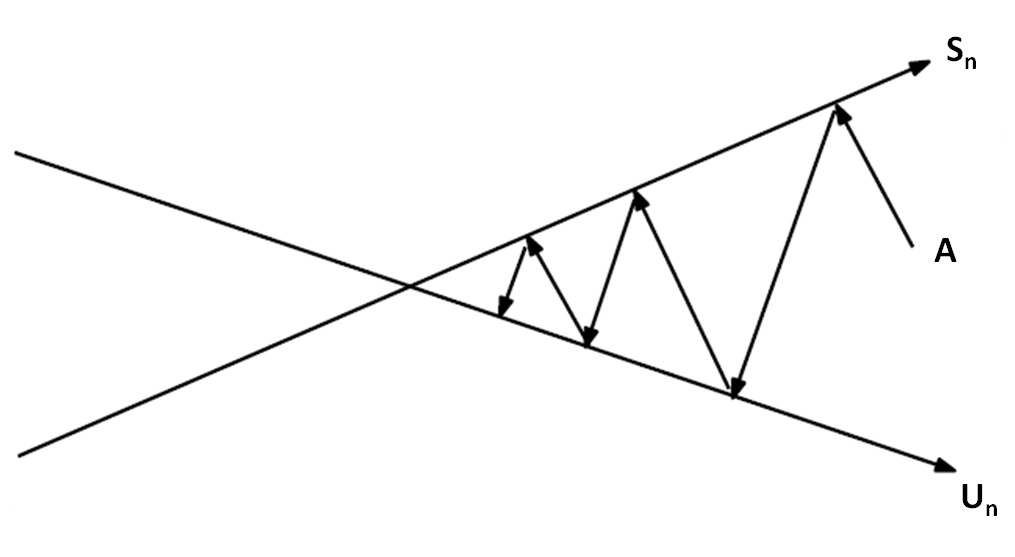
\includegraphics[width=10cm]{metodo_proyecciones2}
\caption{Representación gráfica del método de proyecciones sucesivas.}
\label{metodo_poyecciones}
\end{center}
\end{figure}

Aplicando las proyecciones ya mencionadas de la siguiente manera:
\begin{equation}
\mathbf{A} \leftarrow P_{U}(P_{S}(\mathbf{A}))
\label{def_alg5}
\end{equation}

Los pasos que componen este algoritmo son los siguientes:

\textbf{Paso 0:} Definimos los elementos $\Delta \mathbf{S_{0}}$ y $Y_{0}=\mathbf{C}$ siendo $\mathbf{C}$ una matriz de pseudo-correlación.

\textbf{Paso 1:} $\mathbf{R_{k}}=\mathbf{Y_{k-1}}-\Delta\mathbf{S_{k-1}}$. Siendo $\Delta\mathbf{S_{k-1}}$ la corrección de Dykstra.

\textbf{Paso 2:} $\mathbf{X_{k}}=P_{S}(\mathbf{R_{k}})$.

\textbf{Paso 3:} $\Delta\mathbf{S_{k}}=\mathbf{X_{k}}-\mathbf{R_{k}}$.

\textbf{Paso 4:} $\mathbf{Y_{k}}=P_{U}(\mathbf{X_{k}})$

que converge a la matriz $\mathbf{\widehat{C}}$ cuando $k \longrightarrow \infty$ de manera lineal. Pero para poder asegurar esta convergencia es necesario establecer un criterio de parada a través de un coeficiente de tolerancia. En este caso la definiremos de la siguiente manera: $$\max\lbrace\dfrac{\vert\vert\mathbf{X_{k}}-\mathbf{X_{k-1}}\vert\vert_{\infty}}{\vert\vert\mathbf{X_{k}}\vert\vert_{\infty}},\dfrac{\vert\vert\mathbf{Y_{k}}-\mathbf{Y_{k-1}}\vert\vert_{\infty}}{\vert\vert\mathbf{Y_{k}}\vert\vert_{\infty}},\dfrac{\vert\vert\mathbf{Y_{k}}-\mathbf{X_{k-1}}\vert\vert_{\infty}}{\vert\vert\mathbf{Y_{k}}\vert\vert_{\infty}}\rbrace$$
aplicado después de realizar el paso 4 en cada iteración.

\textbf{\underline{5. Pasha Zusmanovich (2013):}}

Este método de transformación de matrices publicado en \cite{Zusmanovich2013}. Está basado en la teoría de Arnold de deformación de matrices \cite{Arnold1971}, pero a causa de las propiedades de las matrices que tratamos, el algoritmo se reduce al publicado en \cite{Iman1982} con el método de normalización C y también muy similar al publicado en \cite{Rousseeuw1993}. Por lo que no vamos a entrar más en detalle.



\subsection{Metodología del trabajo de tesis doctoral.}

El objetivo de este trabajo de tesis doctoral es desarrollar un método de metaanálisis multivariado que trate de estimar la correlación intra-estudios de la mejor manera posible porque como ya se ha justificado anteriormente, desempeña un papel muy importante a la hora de obtener los estimadores del efecto conjunto a través del fenómeno conocido como borrowing of strength.

Con este fin hemos introducido la imputación múltiple. Esta técnica permite trabajar con valores perdidos de una manera fácil e intuitiva y como en nuestro caso estas correlaciones no suelen ser reportadas y el modelo las asume conocidas, podemos verlas como valores perdidos. Para poder aplicar la imputación múltiple, era necesario probar que los valores perdidos cumplían unas determinadas condiciones. En este caso se puede ver como siguen un mecanismo ignorable (MCAR o MAR) ya que los valores perdidos en la correlación intra-estudios no están relacionados con sus propios valores y ni con los valores de los outcomes recogidos.

La aplicación de la imputación múltiple al metaanálisis multivariado se va a realizar desde dos puntos de vista diferentes. La correlación es una magnitud encargada de cuantificar la relación existente entre dos variables y recorre un espacio de posibles valores acotado, es decir, $\rho \in \left[ -1,1 \right]$ y se calcula a partir de las observaciones de la pareja de variables seleccionada.

Precisamente cada uno de los puntos de vista está relacionado con uno de los dos conceptos previos. En otras palabras:

\paragraph{Punto de vista 1: Datos agrupados.} 
En esta situación los datos que tenemos son las mediciones de los diferentes outcomes por cada grupo de tratamiento y por cada estudio. Como el coeficiente de correlación se calcula a partir de datos individuales, tenemos que idear otra forma de poder obtenerlos. La idea que vamos a seguir es la de las imputaciones múltiples, por lo que tendremos que estimar una serie de valores para cada uno de los coeficientes de correlación. La manera de poder conseguirlos va a ser a partir de una distribución de probabilidad, para lo cual nos apoyaremos en la idea bayesiana de no sólo utilizar la información de los estudios.

Una vez recogida toda la información posible acerca de la relación entre cada pareja de outcomes, tanto la proveniente de los diferentes estudios como aquella ajena a los mismos, vamos a seleccionar de todas las distribuciones de probabilidad aquella que mejor se ajuste y será esta la que utilicemos como distribución predictiva. Se decía antes que nos apoyaríamos en la idea bayesiana para la recogida de información pero en general no podemos utilizar al pie de la letra el teorema de Bayes \ref{bayes}. El motivo es el siguiente, si la distribución a priori y la distribución de los datos no son conjugadas, la distribución predictiva no se puede expresar como una de las ya existente lo que dificulta sobremanera el muestreo.

De esta manera podemos utilizar cualquier distribución de probabilidad: normal truncada, distribución beta, distribución uniforme, etc. Obviamente el intervalo donde se definan estará íntimanete ligado a la información disponible ya que si es lo suficientemente válida, podremos utilizar intervalos $[a,b]\in [-1,1]$. En cambio si dicha información es insuficiente, tendremos que contemplar la posibilidad de que el coeficiente correlación pueda ser cualquiera, es decir, tendremos que definir la distribución de probabilidad en $[-1,1]$.

Tras determinar la distribución para la correlación, deberemos determinar el número de imputaciones $m$. Para ello extraeremos una muestra de $m$ valores independientes utilizando la distribución predictiva para $\rho$, teniendo $m$ matrices de correlación para cada estudio. Posteriormente, mediante las reglas de Rubin \ref{estimador_puntual_imputacion multiple} y \ref{total_var_est_puntual}, combinaremos los valores de las $m$ matrices para obtener una única matriz de correlaciones con su correspondiente variabilidad. Será esta matriz la que utilizaremos para imputar los coeficientes de correlación desconocidos. 

De esta manera ya tenemos determinados todos los elementos necesarios para poder realizar el metaanalisis multivariado y de este modo poder estimar un estimador conjunto para los estimadores del efecto de las diferentes variables de resultado, así como una estimación global de las correlaciones entre las mismas.

\medskip 
\begin{figure}[htb]
\begin{center}
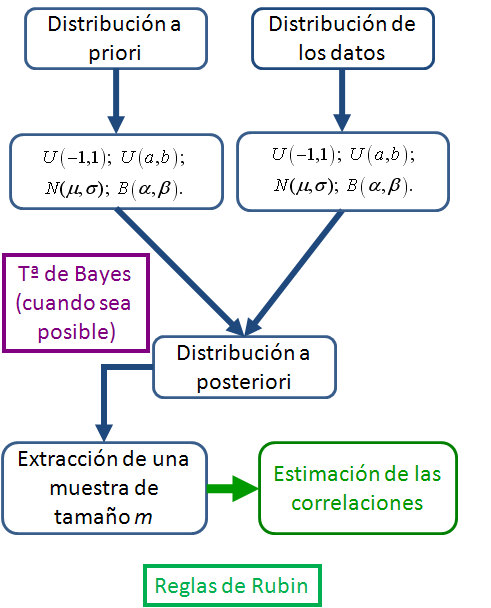
\includegraphics[width=10cm]{Perspectiva1}
\caption{Esquema del análisis con datos agrupados.}
\label{Perspectiva1}
\end{center}
\end{figure}

\paragraph{Punto de vista 2: Datos individuales.}
Aquí vamos a imputar la correlación intra-estudios desde el punto de vista de los datos individuales. Si bien es cierto que en la mayoría de los casos no se dispone de ellos, si se conocen la media y la desviación estándar de los diferentes outcomes en cada uno de los estudios a metaanalizar. Lo que se va a hacer es asumir que la población de los individuos incluidos en el estudio sigue una distribución normal cuya media y desviación estándar es la que viene recogida en la publicación para cada rama de tratamiento.

Una vez establecido el número de imputaciones a obtener, simulamos $m$ muestras independientes a partir de las distribuciones normales cuyas medias y desviaciones estándar serán las que aparezcan en la publicación. El tamaño de estas muestras coincidirá con el tamaño de los grupos de cada publicación. De este modo tendremos $m$ conjuntos de datos individuales por cada estudio a metaanalizar.

El siguiente paso será emplear las reglas de Rubin \ref{estimador_puntual_imputacion multiple} y \ref{total_var_est_puntual} para a partir de las $m$ muestras obtenidos anteriormente, construir un único conjunto de datos individuales que será el que utilicemos para imputar los datos individuales que desconocemos. 

Finalmente, con estos datos individuales podemos calcular el coeficiente de correlación para cada pareja de outcomes en cada uno de los estudios utilizando la fórmula clásica del coeficiente de correlación \ref{formula_corr}. A partir de estos coeficientes, generaríamos las matrices de correlación para cada uno de los estudios y ya tendríamos todos los elementos para poder hacer el metaanálisis multivariado.

\begin{figure}[t]
\begin{center}
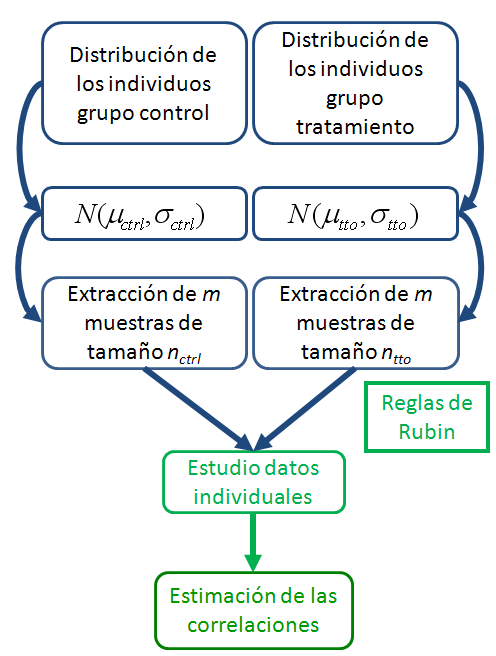
\includegraphics[width=10cm]{Perspectiva2}
\caption{Esquema del análisis con datos individuales.}
\label{Perspectiva2}
\end{center}
\end{figure}

Obviamente para que las propuestas anteriores sean de utilidad, al menos no tienen que ser peores que las técnicas que ya existen y que están recogidas en las secciones anteriores. Por lo tanto vamos a tener que comparar estas dos versiones que utilizan la imputación múltiple con las demás técnicas empleando para estimar los parámetros MLE \ref{mle_mvn} o RMLE \ref{rmle_mvm}: método de los momentos \cite{Jackson2010} y el método con una sola correlación \ref{mvm_alternativo} publicado en \cite{Riley2009} y mediante técnicas bayesianas. 

Para poder hacerlo vamos a emplear dos conjuntos de datos, unos estarán obtenidos mediante simulación para ver como es el comportamiento de las diferentes técnicas en distintos escenarios. Luego lo repetiremos utilizando un conjunto de datos reales formado por estudios publicados en los que se estudia la eficacia y seguridad de potenciadores cognitivos en enfermos de esquizofrenia.

%Como en la inmensa mayoría de los metaanáalisis mulivariados vamos a desconocer las correlaciones %intra-estudio y además ya hemos hablado de su importancia, a la hora deocer a su %estimación es lógico %que se intente evitar la utilización de técnicas que como acabamos de ver, perjudiquen más que ayuden a %una correcta especificación del modelo y por lo tanto evitar %en la medida de lo posible extraer unas %conclusiones nada ajustadas a la realidad. Con lo cual vamos a 

%-----------------------------------------------------------------------------------------------------------------------------------------------------------------------------------------
%----------------------------------------------------------------- CAPÍTULO 3: RESULTADOS ------------------------------------------------------------------------------------------------
%----------------------------------------------------------------------------------------------------------------------------------------------------------------------------------------- 
\chapter{Resultados}\label{cap.resultados}
Érase una vez...
\section{sección1}
Bla bla bla
\subsection{subsección1}
Ble ble ble
\subsubsection{subsubsección1}
Bli bli bli
\paragraph{párrafo1}
Blo blo blo

%-----------------------------------------------------------------------------------------------------------------------------------------------------------------------------------------
%------------------------------------------------------------------ CAPÍTULO 4: DISCUSIÓN ------------------------------------------------------------------------------------------------
%----------------------------------------------------------------------------------------------------------------------------------------------------------------------------------------- 
\chapter{Discusión}\label{cap.discusión}
Érase una vez...
\section{sección1}
Bla bla bla
\subsection{subsección1}
Ble ble ble
\subsubsection{subsubsección1}
Bli bli bli
\paragraph{párrafo1}
Blo blo blo

%-----------------------------------------------------------------------------------------------------------------------------------------------------------------------------------------
%------------------------------------------------------------------ CAPÍTULO 5: CONCLUSIONES ---------------------------------------------------------------------------------------------
%-----------------------------------------------------------------------------------------------------------------------------------------------------------------------------------------
\chapter{Conclusiones}\label{cap.conclusiones}
Érase una vez...
\section{sección1}
Bla bla bla
\subsection{subsección1}
Ble ble ble
\subsubsection{subsubsección1}
Bli bli bli
\paragraph{párrafo1}
Blo blo blo

%-----------------------------------------------------------------------------------------------------------------------------------------------------------------------------------------
%------------------------------ CAPÍTULO 6: BIBLIOGRAFÍA ---------------------------------------------------------------------------------------------------------------------------------
%----------------------------------------------------------------------------------------------------------------------------------------------------------------------------------------- 
\markright{\textit{Capítulo 6: Bibliografía.}}
\chapter{Bibliografía}\label{cap.bibliografía}
\begin{thebibliography}{99}
\bibitem{Cochrane_man} Higgins JPT, Green S (editors). \textit{Cochrane Handbook for Systematic Reviews of Interventions Version 5.0.2} [updated September 2009]. The Cochrane Collaboration, 2009. Available from www.cochrane-handbook.org.
\bibitem{DSMIV1994} American Psychiatric Association. (2000) \textit{Diagnostic and statistical manual of mental disorders} ($4^{th}$ ed., text rev.). Washington, DC.
\bibitem{Zabala2009} Zabala A. et al. Neuropsycological functioning in early-onset first-episode psychosis: comparison of diagnostic subgroups. \textit{European Archives of Psychiatry and Clinical Neuroscience} 2010; 260:225-33.
\bibitem{Reichenberg2009} Reichenberg A. et al. Static and dynamic cognitive deficitsin childhood preceding adult schizophrenia: a 30-year study. \texit{American Journal of Psychiatry} 2010; 167:160-9.
\bibitem{Green2006} Green MF. Cognitive impairment and functional outcome in schizophrenia and bipolar disorder. \textit{Journal of Clinincal Psychiatry} 2006: 67 Suppl 9:3-8; discussion 36-42.
\bibitem{Harvey2009} Harvey P. D. Pharmacological cognitive enhancement in schizophrenia. \textit{Neuropsycology Review} 2009; 19: 324-35.
\bibitem{Ballesteros2008} Ballesteros J. et al. The effectiveness of donepezil for cognitive rehabilitation after traumatic brain injury: a systematic review. \textit{Journal of Head Trauma Rehabilitation} 2008; 23: 171-80.
\bibitem{Chourinard2007} Chourinard S. et al. Oral cholinesterase inhibitor add-on therapy for cognitive enhancement in schizophrenia:a quantitative systematic review, part I. \textit{Clinincal Neuropharmacology} 2007; 30: 169-82.
\bibitem{Stip2007} Stip E. et al. Add-on therapy with acetylcholinesterase inhibitors for memory dysfunction in schizophrenia: a systematic quantitative review, part II. \textit{Clinincal Neuropharmacology} 2007; 30: 218-29.
\bibitem{Ribeiz2010} Ribeiz S. R. et al. Cholinesterase inhibitors as adjunctive therapy in patients with schizophrenia and schizoaffective disorder: a review and meta-analysis of the literature. \textit{CNS Drugs}  2010; 24 (4): 303-17.
\bibitem{Szoke2008} Szoke A. et al. Longitudinal studies of cognition in schizophrenia: meta-analysis. \textit{British Journal of Psychiatry} 2008; 192 (4): 248-57.
\bibitem{Bora2009} Bora E. et al. Cognitive functioning in schizophrenia, schizoaffective disorder and affective psychoses: meta-analytic estudy. \textit{British Journal of Psychiatry} 2009; 195: 475-82.
\bibitem{Singh2009} Sing J. et al. Acetylcholinesterase inhibitors for schizophrenia. \textit{The Cochrane Library} 2009, Issue 4.
\bibitem{Becker2007} Becker B. J. Multivariate Meta-analysis: Contributions of Ingmar Olkin. \textit{Statistical Science} 2007; 22 (3): 401-6.
\bibitem{Berkey1996} Berket C. S. Multiple outcome meta-analysis of clinical trials. \textit{Statistics in Medicine} 1996; 15: 537-57.
\bibitem{Arends2003} Arends L. R. Combining multiple outcome measures in meta-analysis: an application. \textit{Statistics in Medicine} 2003; 22: 1335-53.
\bibitem{Jackson2010} Jackson D. et al. Extending DerSimonian and Laird's methodology to perform multivariate random effects meta-analyses. \textit{Statistics in Medicine} 2010; 29: 1282-97.
\bibitem{Nam2003} Nam I. S. et al. Multivariate meta-analysis. \textit{Statistics in Medicine} 2003; 22: 2309-33.
\bibitem{Jackson2011} Jackson D. et al. Multivariate meta-analysis: Potential and promise. \textit{Statistics in Medicine} 2011; DOI: 10.1002/sim.4172.
\bibitem{Ishak2008} Ishak K. J. et al. Impact of approximating or ignoring within-study covariances in multivariate meta-analyses. \textit{Statistics in Medicine} 2008; 27: 670-86.
\bibitem{Riley2009} Riley R. D. Multivariate meta-analysis: the effect of ignoring within-study correlation. \textit{Journal of Royal Statistical Society: Series A} 2009; 4: 789-811.
\bibitem{Wei2013} Wei Y. et al. Estimating within-study covariances in multivariate meta-analysis with multiple outcomes. \textit{Statistics in Medicine} 2013; 32: 1191-1205. 
\bibitem{Lambert2005} Lambert P. C. et al. How vague is vague? A simulation study of the impact of the use vague prior distributions in MCMC using WinBUGS. \textit{Statistics in Medicine} 2005; 24: 2401-28.
\bibitem{Stata} StataCorp. 2013. \textit{Stata Statistical Software: Release 13.} College Station, TX: StataCorp LP.
\bibitem{R} R Core Team (2013). \textit{R: A language and environment for statistical computing.} R Foundation for Statistical Computing, Vienna, Austria. URL http://www.R-project.org/.
\bibitem{WinBUGS} Lunn, D.J. et al. WinBUGS -- a Bayesian modelling framework: concepts, structure, and extensibility. \textit{Statistics and Computing} 2010; 10:325--337.
\bibitem{Glass1976} Glass GV. Primary, secondary, and meta-analysis of research. \textit{Educational Researcher} 1976; 5: 3-8.
\bibitem{Shadish1994} Shadish W. R. \& Haddock C. K. Combining estimates of effect size. In: Cooper H. \& Hedges L. V., (editors). \textit{The Handbook of Research Synthesis} 1994; New York: Russel Sage Foundation; 261-84.
\bibitem{DerSimonian1986} DerSimonian R. \& Laird N. Meta-Analysis in Clinincal Trials. \textit{Controlled Clinical Trials} 1986; 7: 177-88.
\bibitem{Riley2007} Riley R. D. et al. An evaluation of bivariate random-effects meta-analysis for the joint synthesis of two correlated outcomes. \textit{Statistics in Medicine} 2007; 26: 78-97.
\bibitem{Eysenck1994} Eysenck H. J. Meta-analysis and its problems. \textit{British Medical Journal} 1994; 309: 789-92.
\bibitem{Berkey1998} Berkey C. S et al. Meta-analysis of multiple outcomes by regression with random effects. \textit{Statistics in Medicine} 1998; 17: 2537-2550. 
\bibitem{Higgins1996} Higgins J. P. T. \& Whitehead A. Borrowing strength from external trials in a meta-analysis. \textit{Statistics in Medicine} 1996; 15: 2733-2749.
\bibitem{Mavridis2011} Mavridis D. \& Salanti G. A practical introduction to multivariate meta-analysis. \textit{Statistical Methods in Medical Research} 2011; 22 (2): 133-158.
\bibitem{Ritz2008} Ritz J. et al. Multivariate meta-analysis for data consortia, individual patient meta-analysys, and pooling projects. \textit{Journal of Statistical Planning and Inference} 2008; 138: 1919-1933.
\bibitem{Bujkiewicz2013} Bujkiewicz S. et al. Multivariate meta-analysis of mixed outcomes: a Bayesian approach. \textit{Statistics in Medicine} 2013; 32 (22): 3926-43
\bibitem{Wei2013_2} Wei Y. \& Higgins J. P. T. Bayesian multivariate meta-analysis with multiple outcomes. \textit{Statistics in Medicine} 2013; 32 (17): 2911-34.
\bibitem{Riley2007_2} Riley R. D. et al. Bivariate random effects meta-analysis and the estimation of between-study correlation. \textit{BMC Medical Research Methodology} 2007; 7 (3). \url{http://www.biomedcentral.com/1471-2288/7/3}.
\bibitem{Riley2008} Riley R. D. et al. An alternative model for bivariate random-effects model meta-analysis when the within-study correlations are unknown. \textit{Biostatistics} 2008; 9 (1): 172-86. 
\bibitem{Cox2005} Cox C. Delta method. In \textit{Encyclopedia of Biostatistics} Armitage P. \& Colton T. (eds.) John Wiley \& Sons UK 2003; 22 (14): 2309-33.
\bibitem{Rubin1976} Rubin D. B. Inference and missing data. \textit{Biometrika} 1976; 63 (3): 581-90.
\bibitem{Schafer1998} Schafer J. L: \& Olsen M. K. Multiple Imputation for Multivariate Missing-Data Problems: A Data Analyst's Perspective. \textit{Multivariate Behavioural Research} 1998; 33 (4): 545-71. 
\bibitem{Rubin1987} Rubin D. B. Multiple Imputationfor Nonresponse in Survey. \textit{John Wiley \& Sons} 1987.
\bibitem{VanBuuren2012} Van Buuren S. Flexible Imputation of Missing Data. \textit{CRC Press} 2012.
\bibitem{Rubin1978} Rubin D. B. Bayesian Inference for Causal Effects: The Role of Randomization. \textit{The annals of Statistics} 1978; 6 (1): 34-58.
\bibitem{Rubin1978_2} Rubin D. B. The Phenomenological Bayesian Perspective in Sample Surveys from Finite Populations: Foundations. \textit{Spring Meetings of the Institute for Mathematical Statistics} 1978. 
\bibitem{Rubin1978_3} Rubin D. B. Multiple imputations in sample surveys: a phenomenological Bayesian approach to nonresponse. \textit{Proceedings of the Survey Research Methods Section}, American Statistical Association; 1978: 20-28. 
\bibitem{Rubin1996} Rubin D. B. Multiple imputation after 18+ years. \textit{Journal of the American Statistical Association} 1996; 91 (434): 473-89.
\bibitem{Schafer1997} Schafer J. L. Analysis of incomplete multivariate data. \textit{Champman \& Hall} 1997.
\bibitem{Graham2007} Graham J. W. et al. How Many Imputations are Really Needed? Some Practical CLarifications of Multiple Imputation Theory. \textit{Prevention Science} 2007; 8 (3): 206-13.
\bibitem{Royston2004} Royston P. Multiple imputation of missing values. \textit{The Stata Journal} 2004; 4 (3): 227-41.
\bibitem{Bodner2008} Bodner T. E. What Improves with Increased Missing Data Imputations? \textit{Structural Equation Modelling} 2008; 15: 651-75.
\bibitem{Longford2005} Longford N. Missing Data and small-area estimation: Modern analytical equipment for the survey statistician. \textit{Springer} 2005.
\bibitem{Barnard2000} Barnard J., McCulloch R. \& Meng X. I. Modelling Covariance Matrices in Terms of Standard Deviations and Correlations, with Application to Shrinkage. \textit{Statistica Sinica} 2000; 10: 1281-1311.
\bibitem{Rousseeuw1994} Rousseeuw P. J. \& Molenberghs G. The Shape of Correlation Matrices. \textit{The American Statistician} 1994; 48 (4):276-279.
\bibitem{Rousseeuw1993} Rousseeuw P. J. \& Molenberghs G. Transformations of non positive semidifinite correlations matrices. \textit{Communications in Statistics - Theory and Methods}1993; 22 (4): 965-984.
\bibitem{Joe2005} Joe H. Generating random correlation matrices based on partial correlations. \textit{Journal of Multivariate Analysis} 2005; 97: 2177-2189.
\bibitem{Hurliman2012} Hürlimann W. Positive Semi-definite Correlation Matrices: Recursive Algorithmic Generation and Volume Measure. \textit{Pure Mathematical Sciences} 2012; 1 (3): 137-149.
\bibitem{Iman1982} Iman R. L. \& Davenport J. M. An Iterative Algorithm to Produce a Positive Definite Correlation Matrix from an "Approximate Correlation Matrix" (With a Program User's Guide). \textit{Report SAND-81-1376, Sandia National Laboratories} 1982.
\bibitem{Rebonato2000} Rebonato R. \& Jäckel P. The most general methodology to create a valid correlation matrix for risk management and option pricing purposes. \textit{Journal of Risk} 1999; 2 (2): 17-28.
\bibitem{Pinheiro1996} Pinheiro J. C. \& Bates D. M. Unconstrained parametrizations for variance-covariance matrices. \textit{Statistics and Computing} 1996; 6: 289-296.
\bibitem{Higham2002} Higham N. J. Computing the nearest correlation matrix - a problem of finance. \textit{IMA Journal of Numerical Analysis} 2002; 22: 329-343. 
\bibitem{Luenberger1969} Optimization by Vector Space Methods. \textit{Wiley} 1969.
\bibitem{Han1988} S. P. Han. A succesive projection method. \textit{Mathematical Programming} 1988; 40: 1-14.
\bibitem{Dykstra1983} R. L. Dykstra. An algorithm for restricted least squares regression. \textit{Journal of American Statistical Association} 1983; 78 (384): 837-842.
\bibitem{Zusmanovich2013} P. Zusmanovich. On near and the nearest correlation matrix. \textit{Journal of Nonlinear Mathematical Physics} 2013; 20: 431-439.
\bibitem{Arnold1971} V. I. Arnold. On matrices depending on paramters
\end{thebibliography}

%----------------------------------------------------------------------------------------------------
%------------------------------ CAPÍTULO 7: ANEXOS --------------------------------------------
%----------------------------------------------------------------------------------------------------
\markright{\textit{Anexo 1. Programación de la simulación.}}
\chapter{Anexo 1. Programación de la simulación}\label{cap.simulacion}
A continuación se van a presentar los códigos en R necesarios para poder replicar las diferentes simulaciones realizadas en la sección $2.2.6$
\section{Simulación de estudios con datos individuales.}
\subsubsection{Código para la simulación de estudios con datos individuales}
{\tiny
\begin{verbatim}
################################################################################################################################
#################################FUNCION 1: SIMULACION DE ESTUDIOS CON DATOS INDIVIDUALES#######################################
################################################################################################################################

# PARAMTEROS IMPORTANTES EN LA SIMULACION:
# 1. Numero de estudios
# 2. Numero de variables
# 3. Tamano de la muestra
# 4. Media grupo tratamiento
# 5. SD grupo tratamiento
# 6. Media grupo control
# 7. SD grupo control.
# 8. Correlacion entre outcomes.

# VALORES DE LOS PARAMETROS
# Numero de estudios: 5, 10, 15, 25, 50.
# Numero de variables: 2, 4, 6.
# Tamano de la muestra: 20, 40, 60, 80, 100 (la mitad en cada rama) 
# Media grupo tratamiento distribuciones normales N(media,sd^2)
#   Var 1 (PANSS Total): N(60.56,16.97^2) # Rev Psiquiatr Salud Ment (Barc.) 2009;2(4):160-168 Punt min = 30; Punt max = 210.
#   Var 2 (PANSS Positiva): N(13.65,5.90^2) # Rev Psiquiatr Salud Ment (Barc.) 2009;2(4):160-168 Punt min = 7; Punt max= 49.
#   Var 3 (PANSS Negativa): N(17.82,6.92^2) # Rev Psiquiatr Salud Ment (Barc.) 2009;2(4):160-168 Punt min = 7; Punt max= 49.
#   Var 4 (PANSS General): N(29.01,8.15^2) # Rev Psiquiatr Salud Ment (Barc.) 2009;2(4):160-168 Punt min = 16; Punt max= 112.
#   Var 5 (HAMD): N(17.3,5.5) # Psychiatry Research 144 (2006) 57-63 Punt min = 0;Punt max= 52.
#   Var 6 (Calgary): N(17,15.3^2) # Banco de instrumentos para la psiquiatria clinica Punt min = 0; Punt max= 27.
# Media grupo control distribuciones normales N(media,sd^2)
# Parametros basados en las muestras de las publicaciones correspondientes necesarios para que no haya
# solapamiento entre los intervalos de confianza al 95% de los dos grupos.
#   Var 1 (PANSS Total): N(50.5,20.3^2) Punt min = 30; Punt max = 210.
#   Var 2 (PANSS Positiva): N(9,9.3^2) Punt min = 7; Punt max= 49.
#   Var 3 (PANSS Negativa): N(11.5,7^2) Punt min = 7; Punt max= 49.
#   Var 4 (PANSS General): N(20,9.15^2) Punt min = 16; Punt max= 112.
#   Var 5 (HAMD): N(8.4,4.6^2) Punt min = 0;Punt max= 52.
#   Var 6 (Calgary): N(3,4.2^2) Punt min = 0; Punt max= 27.
# Correlacion entre outcomes: 0, 0.1, 0.3, 0.5, 0.7, 0.9. 

# Librerias necesarias para la simulacion
library(truncdist) # De esta manera se truncaran los valores de las diferentes puntuaciones, para que no se simulen puntuaciones
# fuera de rango.
# Semilla para poder replicar los datos
set.seed(18052013)

# Funcion que va a simular los datos en el escenario que queramos

simulacion_datos <- function(n.estudios,n.vars,tamano.muestra,semilla,replicaciones){
  # Control de los paramtero de la funcion
  if(n.estudios > 50 || n.estudios < 5){
    stop("Numero de estudios incorrecto")
  }
  if((n.vars > 12 || n.vars < 4) && is.integer(n.vars/2)!= TRUE){
    stop("Numero de variables por estudio incorrecto")
  }
  if(tamano.muestra > 100 || tamano.muestra < 20){
    stop("Tamano de muestra incorrecto")
  }
  if(replicaciones < 5 || replicaciones > 150){
    stop("El numero de replicaciones es incorrecto")
  }
  # Funcion propiamente dicha
  database <- vector("list",replicaciones) # Lista donde se almacenaran las replicaciones del escenario deseado
  for(i in 1:replicaciones){
    database[[i]] <- vector("list",n.estudios) # Lista donde se almacenaran el número de estudios determinado
    set.seed(semilla)
    for(j in 1:n.estudios){
      Var1.Trat <- round(rtrunc(tamano.muestra,spec="norm",a=30,b=210,mean=60.56,sd=16.97),0) # Puntuaciones PANSS total en 
                                                                                              # tratamiento
      Var1.Ctrl <- round(rtrunc(tamano.muestra,spec="norm",a=30,b=210,mean=50.5,sd=20.3),0) # Puntuaciones PANSS total en 
                                                                                            # control
      Var2.Trat <- round(rtrunc(tamano.muestra,spec="norm",a=7,b=49,mean=13.65,sd=5.9),0) # Puntuaciones PANSS positiva 
                                                                                          # tratamiento
      Var2.Ctrl <- round(rtrunc(tamano.muestra,spec="norm",a=7,b=49,mean=9,sd=9.3),0) # Puntuaciones PANSS positiva control
      Var3.Trat <- round(rtrunc(tamano.muestra,spec="norm",a=7,b=49,mean=17.82,sd=6.92),0) # Puntuaciones PANSS negativa 
                                                                                           # tratamiento
      Var3.Ctrl <- round(rtrunc(tamano.muestra,spec="norm",a=7,b=49,mean=11,sd=5.7),0) # Puntuaciones PANSS negativa control
      Var4.Trat <- round(rtrunc(tamano.muestra,spec="norm",a=16,b=112,mean=29.01,sd=8.15),0) # Puntuaciones PANSS general 
                                                                                             # tratamiento
      Var4.Ctrl <- round(rtrunc(tamano.muestra,spec="norm",a=16,b=112,mean=20.9,sd=9.15),0) # Puntuaciones PANSS general control
      Var5.Trat <- round(rtrunc(tamano.muestra,spec="norm",a=0,b=52,mean=17.3,sd=5.5),0) # Puntuaciones HAMD tratamiento
      Var5.Ctrl <- round(rtrunc(tamano.muestra,spec="norm",a=0,b=52,mean=8.4,sd=4.6),0) # Puntuaciones HAMD control
      Var6.Trat <- round(rtrunc(tamano.muestra,spec="norm",a=0,b=27,mean=17.15,sd=15.3),0) # Puntuaciones Calgary tratamiento
      Var6.Ctrl <- round(rtrunc(tamano.muestra,spec="norm",a=0,b=27,mean=3,sd=4.2),0) # Puntuaciones Calgary control
      database[[i]][[j]] <- as.data.frame(cbind(Var1.Trat,Var1.Ctrl,Var2.Trat,Var2.Ctrl,Var3.Trat,Var3.Ctrl,Var4.Trat,
                                                Var4.Ctrl,Var5.Trat,Var5.Ctrl,Var6.Trat,Var6.Ctrl))
      semilla <- semilla + 1
    }
  }
  # Para dimensionar en funcion del numero de variables requeridas
  for(i in 1:replicaciones){
    for(j in 1:n.estudios){
      if(n.vars == 4 || n.vars == 6 || n.vars == 8 || n.vars == 10 || n.vars == 12){
        database[[i]][[j]] <- database[[i]][[j]][,c(1:n.vars)]
      } else {
        stop("Numero de variables incorrecto")
      }
    }
  }
  return(database)
}

###############################################################################################################################
###################FUNCION 2: SIMULACION DE ESTUDIOS CON DATOS INDIVIDUALES (SIMPLIFICADA)#####################################
###############################################################################################################################

# COMPARACION DE LOS MÉTODOS DE METAANALISIS DESARROLLADOS FRENTE A LOS PROPUESTOS EN LA TESIS.
# LA COMPARACION SE HARA MEDIANTE SIMULACION BAJO DIFERENTES CONDICIONES.

# FECHA INICIO: 4 / MARZO / 2014
# FECHA FIN: 10/ MARZO / 2014

# PARAMTEROS IMPORTANTES EN LA SIMULACION:
# 1. Numero de estudios
# 2. Numero de variables
# 3. Tamaño de la muestra
# 4. Media grupo tratamiento
# 5. SD grupo tratamiento
# 6. Media grupo control
# 7. SD grupo control.
# 8. Correlacion entre outcomes.

# VALORES DE LOS PARAMETROS
# Numero de estudios: 5, 10, 15, 25, 50.
# Numero de variables: 2, 4, 6.
# Tamano de la muestra: 20, 40, 60, 80, 100 (la mitad en cada rama) 
# Media grupo tratamiento distribuciones normales N(media,sd^2)
#   Var 1 (PANSS Total): N(60.56,16.97^2) # Rev Psiquiatr Salud Ment (Barc.) 2009;2(4):160-168 Punt min = 30; Punt max = 210.
#   Var 2 (PANSS Positiva): N(13.65,5.90^2) # Rev Psiquiatr Salud Ment (Barc.) 2009;2(4):160-168 Punt min = 7; Punt max= 49.
#   Var 3 (PANSS Negativa): N(17.82,6.92^2) # Rev Psiquiatr Salud Ment (Barc.) 2009;2(4):160-168 Punt min = 7; Punt max= 49.
#   Var 4 (PANSS General): N(29.01,8.15^2) # Rev Psiquiatr Salud Ment (Barc.) 2009;2(4):160-168 Punt min = 16; Punt max= 112.
#   Var 5 (HAMD): N(17.3,5.5) # Psychiatry Research 144 (2006) 57-63 Punt min = 0;Punt max= 52.
#   Var 6 (Calgary): N(17,15.3^2) # Banco de instrumentos para la psiquiatria clinica Punt min = 0; Punt max= 27.
# Media grupo control distribuciones normales N(media,sd^2)
# Parametros basados en las muestras de las publicaciones correspondientes necesarios para que no haya
# solapamiento entre los intervalos de confianza al 95% de los dos grupos.
#   Var 1 (PANSS Total): N(50.5,20.3^2) Punt min = 30; Punt max = 210.
#   Var 2 (PANSS Positiva): N(9,9.3^2) Punt min = 7; Punt max= 49.
#   Var 3 (PANSS Negativa): N(11.5,7^2) Punt min = 7; Punt max= 49.
#   Var 4 (PANSS General): N(20,9.15^2) Punt min = 16; Punt max= 112.
#   Var 5 (HAMD): N(8.4,4.6^2) Punt min = 0;Punt max= 52.
#   Var 6 (Calgary): N(3,4.2^2) Punt min = 0; Punt max= 27.
# Correlacion entre outcomes: 0, 0.1, 0.3, 0.5, 0.7, 0.9. 

# Librerias necesarias para la simulacion
library(truncdist) # De esta manera se truncaran los valores de las diferentes puntuaciones, para que no se simulen puntuaciones
# fuera de rango.
# Semilla para poder replicar los datos
set.seed(18052013)

# Función que va a simular los datos en el escenario que queramos

simulacion_datos2 <- function(n.estudios,n.vars,tamano.muestra,semilla,replicaciones){
  # Control de los paramtero de la funcion
  if(n.estudios > 50 || n.estudios < 5){
    stop("Numero de estudios incorrecto")
  }
  if((n.vars > 12 || n.vars < 4) && is.integer(n.vars/2)!= TRUE){
    stop("Numero de variables por estudio incorrecto")
  }
  if(tamano.muestra > 100 || tamano.muestra < 20){
    stop("Tamano de muestra incorrecto")
  }
  if(replicaciones < 5 || replicaciones > 150){
    stop("El numero de replicaciones es incorrecto")
  }
  # Funcion propiamente dicha
  database <- vector("list",replicaciones) # Lista donde se almacenaran las replicaciones del escenario deseado
  for(i in 1:replicaciones){
    database[[i]] <- vector("list",n.estudios) # Lista donde se almacenaran el número de estudios determinado
    set.seed(semilla)
    Var1.Trat <- round(rtrunc(tamano.muestra,spec="norm",a=30,b=210,mean=60.56,sd=16.97),0) # Puntuaciones PANSS total en 
                                                                                            # tratamiento
    Var1.Ctrl <- round(rtrunc(tamano.muestra,spec="norm",a=30,b=210,mean=50.5,sd=20.3),0) # Puntuaciones PANSS total en control
    Var2.Trat <- round(rtrunc(tamano.muestra,spec="norm",a=7,b=49,mean=13.65,sd=5.9),0) # Puntuaciones PANSS positiva 
                                                                                        # tratamiento
    Var2.Ctrl <- round(rtrunc(tamano.muestra,spec="norm",a=7,b=49,mean=9,sd=9.3),0) # Puntuaciones PANSS positiva control
    Var3.Trat <- round(rtrunc(tamano.muestra,spec="norm",a=7,b=49,mean=17.82,sd=6.92),0) # Puntuaciones PANSS negativa 
                                                                                         # tratamiento
    Var3.Ctrl <- round(rtrunc(tamano.muestra,spec="norm",a=7,b=49,mean=11,sd=5.7),0) # Puntuaciones PANSS negativa control
    Var4.Trat <- round(rtrunc(tamano.muestra,spec="norm",a=16,b=112,mean=29.01,sd=8.15),0) # Puntuaciones PANSS general 
                                                                                           # tratamiento
    Var4.Ctrl <- round(rtrunc(tamano.muestra,spec="norm",a=16,b=112,mean=20.9,sd=9.15),0) # Puntuaciones PANSS general control
    Var5.Trat <- round(rtrunc(tamano.muestra,spec="norm",a=0,b=52,mean=17.3,sd=5.5),0) # Puntuaciones HAMD tratamiento
    Var5.Ctrl <- round(rtrunc(tamano.muestra,spec="norm",a=0,b=52,mean=8.4,sd=4.6),0) # Puntuaciones HAMD control
    Var6.Trat <- round(rtrunc(tamano.muestra,spec="norm",a=0,b=27,mean=17.15,sd=15.3),0) # Puntuaciones Calgary tratamiento
    Var6.Ctrl <- round(rtrunc(tamano.muestra,spec="norm",a=0,b=27,mean=3,sd=4.2),0) # Puntuaciones Calgary control
    database[[i]] <- as.data.frame(cbind(Var1.Trat,Var1.Ctrl,Var2.Trat,Var2.Ctrl,Var3.Trat,Var3.Ctrl,Var4.Trat,
                                         Var4.Ctrl,Var5.Trat,Var5.Ctrl,Var6.Trat,Var6.Ctrl))
    semilla <- semilla + (n.estudios) 
  }
  for(i in 1:replicaciones){
    if(n.vars == 4 || n.vars == 6 || n.vars == 8 || n.vars == 10 || n.vars == 12){
      database[[i]] <- database[[i]][,c(1:n.vars)]
    } else {
      stop("Numero de variables incorrecto")
    }
  }
  return(database)
}
\end{verbatim}}
\newpage

\subsection{Escenario con dos outcomes en cada estudio.}

\subsubsection{Código para el cálculo del estimador del efecto y desviación estándar en cada uno de los estudios}
{\tiny
\begin{verbatim}
##############################################################################################################################
####################FUNCION 3: g DE HEDGES' DE UNA SIMULACION CON REPLICACIONES (SIMPLIFICADA)################################
##############################################################################################################################

g_hedges_simulacion2 <- function(n.estudios=5,n.vars=4,tamano.muestra=20,semilla=18052013,replicaciones=5,correlacion=0){
  library(compute.es)
  datos <- simulacion_datos2(n.estudios,n.vars,tamano.muestra,semilla,replicaciones) 
  datos_meta <- diag(0,replicaciones,n.vars+1)
  for(i in 1:replicaciones){
    g1 <- mes(mean(datos[[i]][,1]),sd(datos[[i]][,1]),tamano.muestra,mean(datos[[i]][,2]),sd(datos[[i]][,2]),tamano.muestra)
          [12][,1]
    g2 <- mes(mean(datos[[i]][,3]),sd(datos[[i]][,3]),tamano.muestra,mean(datos[[i]][,4]),sd(datos[[i]][,4]),tamano.muestra)
          [12][,1]
    var.g1 <- mes(mean(datos[[i]][,1]),sd(datos[[i]][,1]),tamano.muestra,mean(datos[[i]][,2]),sd(datos[[i]][,2]),tamano.muestra)
              [13][,1]
    var.g2 <- mes(mean(datos[[i]][,3]),sd(datos[[i]][,3]),tamano.muestra,mean(datos[[i]][,4]),sd(datos[[i]][,4]),tamano.muestra)
              [13][,1]
    covar.g1g2 <- correlacion*sqrt(var.g1)*sqrt(var.g2)
    input <- c(g1,g2,var.g1,covar.g1g2,var.g2)
    datos_meta[i,] <- input
  }
  colnames(datos_meta) <- c("g1","g2","var.g1","covar.g1g2","var.g2")
  return(as.data.frame(datos_meta))
}

##############################################################################################################################
##########################FUNCION 4: g DE HEDGES' DE UNA SIMULACION CON REPLICACIONES#########################################
##############################################################################################################################

g_hedges_simulacion <- function(n.estudios=5,n.vars=4,tamano.muestra=20,semilla=18052013,replicaciones=5,correlacion=0){
  datos <- simulacion_datos(n.estudios,n.vars,tamano.muestra,semilla,replicaciones)
  library(compute.es)
  # g1 <- vector(mode="numeric",length=replicaciones)
  # g2 <- vector(mode="numeric",length=replicaciones)
  # var.g1 <- vector(mode="numeric",length=replicaciones)
  # var.g2 <- vector(mode="numeric",length=replicaciones)
  # covar.g1g2 <- vector(mode="numeric",length=replicaciones) 
  datos_meta <- vector("list",replicaciones)
  g1 <- vector(mode="numeric",length=n.estudios)
  g2 <- vector(mode="numeric",length=n.estudios)
  var.g1 <- vector(mode="numeric",length=n.estudios)
  var.g2 <- vector(mode="numeric",length=n.estudios)
  covar.g1g2 <- vector(mode="numeric",length=n.estudios) 
  for(i in 1:replicaciones){
    for(j in 1:n.estudios){
      g1[j] <- mes(mean(datos[[i]][[j]][,1]),sd(datos[[i]][[j]][,1]),tamano.muestra,mean(datos[[i]][[j]][,2]),
                   sd(datos[[i]][[j]][,2]),tamano.muestra)[12][,1]
      g2[j] <- mes(mean(datos[[i]][[j]][,3]),sd(datos[[i]][[j]][,3]),tamano.muestra,mean(datos[[i]][[j]][,4]),
                   sd(datos[[i]][[j]][,4]),tamano.muestra)[12][,1]
      var.g1[j] <- mes(mean(datos[[i]][[j]][,1]),sd(datos[[i]][[j]][,1]),tamano.muestra,mean(datos[[i]][[j]][,2]),
                   sd(datos[[i]][[j]][,2]),tamano.muestra)[13][,1]
      var.g2[j] <- mes(mean(datos[[i]][[j]][,3]),sd(datos[[i]][[j]][,3]),tamano.muestra,mean(datos[[i]][[j]][,4]),
                   sd(datos[[i]][[j]][,4]),tamano.muestra)[13][,1]
      covar.g1g2[j] <- correlacion*sqrt(var.g1[j])*sqrt(var.g2[j])
      input <- cbind(g1,g2,var.g1,covar.g1g2,var.g2)
    }
    datos_meta[[i]] <- as.data.frame(input)
  }
  return(datos_meta)
}

\end{verbatim}}
\newpage

\subsubsection{Código para la realización del metaanálisis bivariado empleando cada uno de los conjuntos de estudios simulados.}
{\tiny
\begin{verbatim}
##############################################################################################################################
##########################FUNCION 5: METAANALISIS MULTIVARIADO DE SIMULACION (MODIFICADA)#####################################
##############################################################################################################################

###############
# FUNCION 5.1 #
###############

#datos <- g_hedges_simulacion2(n.estudios=5,n.vars=4,tamano.muestra=20,semilla=18052013,replicaciones=5,correlacion=0)

meta_multi_simulacion2 <- function(data,metodo="reml"){
  library(mvmeta)
  meta_multi <- mvmeta(cbind(g1,g2),as.data.frame(data)[3:5],data=data,method=metodo)
  coeficientes <- meta_multi$coefficients
  coeficientes_inferencia <- summary(meta_multi)$coefficients
  coeficientes_var_cov <- summary(meta_multi)$corRandom
  output <- list(coefs=coeficientes,inferencia=coeficientes_inferencia,var_cov=coeficientes_var_cov)
  return(output)
}
###############
# FUNCION 5.2 #
###############

meta_multi_simulacion2_bis <- function(n.estudios=5,n.vars=4,tamano.muestra=20,semilla=18052013,replicaciones=5,correlacion=0,
                                       metodo="reml"){
  library(mvmeta)
  datos <- g_hedges_simulacion2(n.estudios=5,n.vars=4,tamano.muestra=20,semilla=18052013,replicaciones=5,correlacion=0)
  data <- as.data.frame(datos)
  meta_multi <- mvmeta(cbind(g1,g2),as.data.frame(data)[3:5],data=data,method=metodo)
  coeficientes <- meta_multi$coefficients
  coeficientes_inferencia <- summary(meta_multi)$coefficients
  coeficientes_var_cov <- summary(meta_multi)$corRandom
  output <- list(coefs=coeficientes,inferencia=coeficientes_inferencia,var_cov=coeficientes_var_cov)
  return(output)  
}
##############################################################################################################################
##########################FUNCION 6: METAANALISIS MULTIVARIADO DE SIMULACION (UNO POR REPLICACION)############################
##############################################################################################################################

###############
# FUNCION 6.1 #
###############

#datos <- g_hedges_simulacion(n.estudios=5,n.vars=4,tamano.muestra=20,semilla=18052013,replicaciones=5,correlacion=0)

meta_multi_simulacion <- function(data,metodo="reml",replicaciones=5){
  library(mvmeta)
  meta_multi <- vector(mode="list",length=replicaciones)
  for(i in 1:length(data)){
    datos <- data[[i]]
    meta_resultados <- mvmeta(cbind(g1,g2),S=as.data.frame(data)[3:5],data=datos,method=metodo)
    coeficientes <- meta_resultados$coefficients
    coeficientes_inferencia <- summary(meta_resultados)$coefficients
    coeficientes_var_cov <- summary(meta_resultados)$corRandom
    meta_multi[[i]] <- list(dat=data[[i]],coefs=coeficientes,inferencia=coeficientes_inferencia,var_cov=coeficientes_var_cov)
  }
  return(meta_multi)  
}
###############
# FUNCION 6.2 #
###############

meta_multi_simulacion_bis <- function(n.estudios=5,n.vars=4,tamano.muestra=20,semilla=18052013,replicaciones=5,correlacion=0,
                                         metodo="reml"){
  library(mvmeta)
  datos <- g_hedges_simulacion(n.estudios,n.vars,tamano.muestra,semilla,replicaciones,correlacion)
  meta_multi <- vector(mode="list",length=replicaciones)
  for(i in 1:replicaciones){
    data <- as.data.frame(datos[[i]])
    meta_resultados <- mvmeta(cbind(g1,g2),S=as.data.frame(data)[3:5],data=data,method=metodo)
    coeficientes <- meta_resultados$coefficients
    coeficientes_inferencia <- summary(meta_resultados)$coefficients
    coeficientes_var_cov <- summary(meta_resultados)$corRandom
    meta_multi[[i]] <- list(dat=datos[[i]],coefs=coeficientes,inferencia=coeficientes_inferencia,var_cov=coeficientes_var_cov)
  }
  return(meta_multi)  
  
}
\end{verbatim}}

\section{Escenario con tres outcomes por estudio.}
\subsubsection{Código para el cálculo del estimador del efecto y desviación estándar en cada uno de los estudios}
{\tiny
\begin{verbatim}
##############################################################################################################################
####################FUNCION 3: g DE HEDGES' DE UNA SIMULACION CON REPLICACIONES (SIMPLIFICADA)################################
##############################################################################################################################

g_hedges_simulacion2_3vars <- function(n.estudios=5,tamano.muestra=20,semilla=18052013,replicaciones=5,correlacion12=0,
                                       correlacion13=0,correlacion23=0){
  library(compute.es)
  n.vars <- 6
  datos <- simulacion_datos2(n.estudios,n.vars,tamano.muestra,semilla,replicaciones) 
  datos_meta <- diag(0,replicaciones,n.vars+3)
  for(i in 1:replicaciones){
    g1 <- mes(mean(datos[[i]][,1]),sd(datos[[i]][,1]),tamano.muestra,mean(datos[[i]][,2]),sd(datos[[i]][,2]),tamano.muestra)
          [12][,1]
    g2 <- mes(mean(datos[[i]][,3]),sd(datos[[i]][,3]),tamano.muestra,mean(datos[[i]][,4]),sd(datos[[i]][,4]),tamano.muestra) 
          [12][,1]
    g3 <- mes(mean(datos[[i]][,5]),sd(datos[[i]][,5]),tamano.muestra,mean(datos[[i]][,6]),sd(datos[[i]][,6]),tamano.muestra)
          [12][,1]
    var.g1 <- mes(mean(datos[[i]][,1]),sd(datos[[i]][,1]),tamano.muestra,mean(datos[[i]][,2]),sd(datos[[i]][,2]),tamano.muestra)
              [13][,1]
    var.g2 <- mes(mean(datos[[i]][,3]),sd(datos[[i]][,3]),tamano.muestra,mean(datos[[i]][,4]),sd(datos[[i]][,4]),tamano.muestra)
              [13][,1]
    var.g3 <- mes(mean(datos[[i]][,5]),sd(datos[[i]][,5]),tamano.muestra,mean(datos[[i]][,6]),sd(datos[[i]][,6]),tamano.muestra)
              [13][,1]
    covar.g1g2 <- correlacion12*sqrt(var.g1)*sqrt(var.g2)
    covar.g1g3 <- correlacion13*sqrt(var.g1)*sqrt(var.g3)
    covar.g2g3 <- correlacion23*sqrt(var.g2)*sqrt(var.g3)
    input <- c(g1,g2,g3,var.g1,covar.g1g2,covar.g1g3,var.g2,covar.g2g3,var.g3)
    datos_meta[i,] <- input
  }
  colnames(datos_meta) <- c("g1","g2","g3","var.g1","covar.g1g2","covar.g1g3","var.g2","covar.g2g3","var.g3")
  return(as.data.frame(datos_meta))
}

##############################################################################################################################
##########################FUNCION 4: g DE HEDGES' DE UNA SIMULACION CON REPLICACIONES#########################################
##############################################################################################################################

g_hedges_simulacion_3vars <- function(n.estudios=5,tamano.muestra=20,semilla=18052013,replicaciones=5,correlacion12=0,
                                      correlacion13=0,correlacion23=0){
  library(compute.es)
  n.vars <- 6
  datos <- simulacion_datos(n.estudios,n.vars,tamano.muestra,semilla,replicaciones)
  datos_meta <- vector("list",replicaciones)
  g1 <- vector(mode="numeric",length=n.estudios)
  g2 <- vector(mode="numeric",length=n.estudios)
  g3 <- vector(mode="numeric",length=n.estudios)
  var.g1 <- vector(mode="numeric",length=n.estudios)
  var.g2 <- vector(mode="numeric",length=n.estudios)
  var.g3 <- vector(mode="numeric",length=n.estudios)
  covar.g1g2 <- vector(mode="numeric",length=n.estudios) 
  covar.g1g3 <- vector(mode="numeric",length=n.estudios)
  covar.g2g3 <- vector(mode="numeric",length=n.estudios)
  for(i in 1:replicaciones){
    for(j in 1:n.estudios){
      g1[j] <- mes(mean(datos[[i]][[j]][,1]),sd(datos[[i]][[j]][,1]),tamano.muestra,mean(datos[[i]][[j]][,2]),
               sd(datos[[i]][[j]][,2]),tamano.muestra)[12][,1]
      g2[j] <- mes(mean(datos[[i]][[j]][,3]),sd(datos[[i]][[j]][,3]),tamano.muestra,mean(datos[[i]][[j]][,4]),
               sd(datos[[i]][[j]][,4]),tamano.muestra)[12][,1]
      g3[j] <- mes(mean(datos[[i]][[j]][,5]),sd(datos[[i]][[j]][,5]),tamano.muestra,mean(datos[[i]][[j]][,6]),
               sd(datos[[i]][[j]][,6]),tamano.muestra)[12][,1]
      var.g1[j] <- mes(mean(datos[[i]][[j]][,1]),sd(datos[[i]][[j]][,1]),tamano.muestra,mean(datos[[i]][[j]][,2]),
                   sd(datos[[i]][[j]][,2]),tamano.muestra)[13][,1]
      var.g2[j] <- mes(mean(datos[[i]][[j]][,3]),sd(datos[[i]][[j]][,3]),tamano.muestra,mean(datos[[i]][[j]][,4]),
                   sd(datos[[i]][[j]][,4]),tamano.muestra)[13][,1]
      var.g3[j] <- mes(mean(datos[[i]][[j]][,5]),sd(datos[[i]][[j]][,5]),tamano.muestra,mean(datos[[i]][[j]][,6]),
                   sd(datos[[i]][[j]][,6]),tamano.muestra)[13][,1]
      covar.g1g2[j] <- correlacion12*sqrt(var.g1[j])*sqrt(var.g2[j])
      covar.g1g3[j] <- correlacion13*sqrt(var.g1[j])*sqrt(var.g3[j])
      covar.g2g3[j] <- correlacion23*sqrt(var.g2[j])*sqrt(var.g3[j])
      input <- cbind(g1,g2,g3,var.g1,covar.g1g2,covar.g1g3,var.g2,covar.g2g3,var.g3)
    }
    datos_meta[[i]] <- as.data.frame(input)
  }
  return(datos_meta)
}
\end{verbatim}}
\newpage
\subsubsection{Código para la realización del metaanálisis multivariado empleando cada uno de los conjuntos de estudios simulados.}
{\tiny
\begin{verbatim}
##############################################################################################################################
##########################FUNCION 5: METAANALISIS MULTIVARIADO DE SIMULACION (MODIFICADA)#####################################
##############################################################################################################################

###############
# FUNCION 5.1 #
###############

#datos <- g_hedges_simulacion2_3vars(n.estudios=5,tamano.muestra=20,semilla=18052013,replicaciones=5,correlacion12=0,
#                                   correlacion13=0,correlacion23=0)

meta_multi_simulacion2_3vars <- function(data,metodo="reml"){
  library(mvmeta)
  meta_multi <- mvmeta(cbind(g1,g2,g3),as.data.frame(data)[4:9],data=data,method=metodo)
  coeficientes <- meta_multi$coefficients
  coeficientes_inferencia <- summary(meta_multi)$coefficients
  coeficientes_var_cov <- summary(meta_multi)$corRandom
  output <- list(coefs=coeficientes,inferencia=coeficientes_inferencia,var_cov=coeficientes_var_cov)
  return(output)
}

###############
# FUNCION 5.2 #
###############

meta_multi_simulacion2_3vars_bis <- function(n.estudios=5,tamano.muestra=20,semilla=18052013,replicaciones=5,correlacion12=0,
                                             correlacion13=0,correlacion23=0,metodo="reml"){
  library(mvmeta)
  datos <- g_hedges_simulacion2_3vars(n.estudios,tamano.muestra,semilla,replicaciones,correlacion12,correlacion13,
                                      correlacion23)
  data <- as.data.frame(datos)
  meta_multi <- mvmeta(cbind(g1,g2,g3),as.data.frame(data)[4:9],data=data,method=metodo)
  coeficientes <- meta_multi$coefficients
  coeficientes_inferencia <- summary(meta_multi)$coefficients
  coeficientes_var_cov <- summary(meta_multi)$corRandom
  output <- list(coefs=coeficientes,inferencia=coeficientes_inferencia,var_cov=coeficientes_var_cov)
  return(output)  
}

##############################################################################################################################
##########################FUNCION 6: METAANALISIS MULTIVARIADO DE SIMULACION (UNO POR REPLICACION)############################
##############################################################################################################################

###############
# FUNCION 6.1 #
###############

#datos <- g_hedges_simulacion_3vars(n.estudios=5,tamano.muestra=20,semilla=18052013,replicaciones=5,correlacion12=0,
#                                    correlacion13=0,correlacion23=0)

meta_multi_simulacion_3vars <- function(data,metodo="reml",replicaciones=5){
  library(mvmeta)
  meta_multi <- vector(mode="list",length=replicaciones)
  for(i in 1:length(data)){
    datos <- data[[i]]
    meta_resultados <- mvmeta(cbind(g1,g2,g3),S=as.data.frame(data)[4:9],data=datos,method=metodo)
    coeficientes <- meta_resultados$coefficients
    coeficientes_inferencia <- summary(meta_resultados)$coefficients
    coeficientes_var_cov <- summary(meta_resultados)$corRandom
    meta_multi[[i]] <- list(dat=data[[i]],coefs=coeficientes,inferencia=coeficientes_inferencia,var_cov=coeficientes_var_cov)
  }
  return(meta_multi)  
}

###############
# FUNCION 6.2 #
###############

meta_multi_simulacion_3_vars_bis <- function(n.estudios=5,tamano.muestra=20,semilla=18052013,replicaciones=5,correlacion12=0,
                                      correlacion13=0,correlacion23=0,metodo="reml"){
  library(mvmeta)
  datos <- g_hedges_simulacion_3vars(n.estudios,tamano.muestra,semilla,replicaciones,correlacion12,
                               correlacion13,correlacion23)
  meta_multi <- vector(mode="list",length=replicaciones)
  for(i in 1:replicaciones){
    data <- as.data.frame(datos[[i]])
    meta_resultados <- mvmeta(cbind(g1,g2,g3),S=as.data.frame(data)[4:9],data=data,method=metodo)
    coeficientes <- meta_resultados$coefficients
    coeficientes_inferencia <- summary(meta_resultados)$coefficients
    coeficientes_var_cov <- summary(meta_resultados)$corRandom
    meta_multi[[i]] <- list(dat=datos[[i]],coefs=coeficientes,inferencia=coeficientes_inferencia,var_cov=coeficientes_var_cov)
  }
  return(meta_multi)  
  
}
\end{verbatim}}

\section{Escenario con cuatro outcomes por estudio.}
\subsubsection{Código para el cálculo del estimador del efecto y desviación estándar en cada uno de los estudios}
{\tiny
\begin{verbatim}
##############################################################################################################################
####################FUNCION 3: g DE HEDGES' DE UNA SIMULACION CON REPLICACIONES (SIMPLIFICADA)################################
##############################################################################################################################

g_hedges_simulacion2_4vars <- function(n.estudios=5,tamano.muestra=20,semilla=18052013,replicaciones=5,correlacion12=0,
                                       correlacion13=0,correlacion14=0,correlacion23=0,correlacion24=0,correlacion34=0){
  library(compute.es)
  n.vars <- 8
  datos <- simulacion_datos2(n.estudios,n.vars,tamano.muestra,semilla,replicaciones) 
  datos_meta <- diag(0,replicaciones,n.vars+6)
  for(i in 1:replicaciones){
    g1 <- mes(mean(datos[[i]][,1]),sd(datos[[i]][,1]),tamano.muestra,mean(datos[[i]][,2]),sd(datos[[i]][,2]),tamano.muestra)
          [12][,1]
    g2 <- mes(mean(datos[[i]][,3]),sd(datos[[i]][,3]),tamano.muestra,mean(datos[[i]][,4]),sd(datos[[i]][,4]),tamano.muestra)
          [12][,1]
    g3 <- mes(mean(datos[[i]][,5]),sd(datos[[i]][,5]),tamano.muestra,mean(datos[[i]][,6]),sd(datos[[i]][,6]),tamano.muestra)
          [12][,1]
    g4 <- mes(mean(datos[[i]][,7]),sd(datos[[i]][,7]),tamano.muestra,mean(datos[[i]][,8]),sd(datos[[i]][,8]),tamano.muestra)
          [12][,1]
    var.g1 <- mes(mean(datos[[i]][,1]),sd(datos[[i]][,1]),tamano.muestra,mean(datos[[i]][,2]),sd(datos[[i]][,2]),tamano.muestra)
              [13][,1]
    var.g2 <- mes(mean(datos[[i]][,3]),sd(datos[[i]][,3]),tamano.muestra,mean(datos[[i]][,4]),sd(datos[[i]][,4]),tamano.muestra)
              [13][,1]
    var.g3 <- mes(mean(datos[[i]][,5]),sd(datos[[i]][,5]),tamano.muestra,mean(datos[[i]][,6]),sd(datos[[i]][,6]),tamano.muestra)
              [13][,1]
    var.g4 <- mes(mean(datos[[i]][,7]),sd(datos[[i]][,7]),tamano.muestra,mean(datos[[i]][,8]),sd(datos[[i]][,8]),tamano.muestra)
              [13][,1]
    covar.g1g2 <- correlacion12*sqrt(var.g1)*sqrt(var.g2)
    covar.g1g3 <- correlacion13*sqrt(var.g1)*sqrt(var.g3)
    covar.g1g4 <- correlacion14*sqrt(var.g1)*sqrt(var.g4)
    covar.g2g3 <- correlacion23*sqrt(var.g2)*sqrt(var.g3)
    covar.g2g4 <- correlacion24*sqrt(var.g2)*sqrt(var.g4)
    covar.g3g4 <- correlacion34*sqrt(var.g3)*sqrt(var.g4)
    input <- c(g1,g2,g3,g4,var.g1,covar.g1g2,covar.g1g3,covar.g1g4,var.g2,covar.g2g3,covar.g2g4,var.g3,covar.g3g4,var.g4)
    datos_meta[i,] <- input
  }
  colnames(datos_meta) <- c("g1","g2","g3","g4","var.g1","covar.g1g2","covar.g1g3","covar.g1g4","var.g2","covar.g2g3",
                            "covar.g2g4","var.g3","var.g3g4","var.g4")
  return(as.data.frame(datos_meta))
}

##############################################################################################################################
##########################FUNCION 4: g DE HEDGES' DE UNA SIMULACION CON REPLICACIONES#########################################
##############################################################################################################################

g_hedges_simulacion_4vars <- function(n.estudios=5,tamano.muestra=20,semilla=18052013,replicaciones=5,correlacion12=0,
                                      correlacion13=0,correlacion14=0,correlacion23=0,correlacion24=0,correlacion34=0){
  library(compute.es)
  n.vars <- 8
  datos <- simulacion_datos(n.estudios,n.vars,tamano.muestra,semilla,replicaciones)
  datos_meta <- vector("list",replicaciones)
  g1 <- vector(mode="numeric",length=n.estudios)
  g2 <- vector(mode="numeric",length=n.estudios)
  g3 <- vector(mode="numeric",length=n.estudios)
  g4 <- vector(mode="numeric",length=n.estudios)
  var.g1 <- vector(mode="numeric",length=n.estudios)
  var.g2 <- vector(mode="numeric",length=n.estudios)
  var.g3 <- vector(mode="numeric",length=n.estudios)
  var.g4 <- vector(mode="numeric",length=n.estudios)
  covar.g1g2 <- vector(mode="numeric",length=n.estudios) 
  covar.g1g3 <- vector(mode="numeric",length=n.estudios)
  covar.g1g4 <- vector(mode="numeric",length=n.estudios) 
  covar.g2g3 <- vector(mode="numeric",length=n.estudios)
  covar.g2g4 <- vector(mode="numeric",length=n.estudios) 
  covar.g3g4 <- vector(mode="numeric",length=n.estudios) 
  for(i in 1:replicaciones){
    for(j in 1:n.estudios){
      g1[j] <- mes(mean(datos[[i]][[j]][,1]),sd(datos[[i]][[j]][,1]),tamano.muestra,mean(datos[[i]][[j]][,2]),
               sd(datos[[i]][[j]][,2]),tamano.muestra)[12][,1]
      g2[j] <- mes(mean(datos[[i]][[j]][,3]),sd(datos[[i]][[j]][,3]),tamano.muestra,mean(datos[[i]][[j]][,4]),
               sd(datos[[i]][[j]][,4]),tamano.muestra)[12][,1]
      g3[j] <- mes(mean(datos[[i]][[j]][,5]),sd(datos[[i]][[j]][,5]),tamano.muestra,mean(datos[[i]][[j]][,6]),
               sd(datos[[i]][[j]][,6]),tamano.muestra)[12][,1]
      g4[j] <- mes(mean(datos[[i]][[j]][,7]),sd(datos[[i]][[j]][,7]),tamano.muestra,mean(datos[[i]][[j]][,8]),
               sd(datos[[i]][[j]][,8]),tamano.muestra)[12][,1]
      var.g1[j] <- mes(mean(datos[[i]][[j]][,1]),sd(datos[[i]][[j]][,1]),tamano.muestra,mean(datos[[i]][[j]][,2]),
                   sd(datos[[i]][[j]][,2]),tamano.muestra)[13][,1]
      var.g2[j] <- mes(mean(datos[[i]][[j]][,3]),sd(datos[[i]][[j]][,3]),tamano.muestra,mean(datos[[i]][[j]][,4]),
                   sd(datos[[i]][[j]][,4]),tamano.muestra)[13][,1]
      var.g3[j] <- mes(mean(datos[[i]][[j]][,5]),sd(datos[[i]][[j]][,5]),tamano.muestra,mean(datos[[i]][[j]][,6]),
                   sd(datos[[i]][[j]][,6]),tamano.muestra)[13][,1]
      var.g4[j] <- mes(mean(datos[[i]][[j]][,7]),sd(datos[[i]][[j]][,7]),tamano.muestra,mean(datos[[i]][[j]][,8]),
                   sd(datos[[i]][[j]][,8]),tamano.muestra)[13][,1]
      covar.g1g2[j] <- correlacion12*sqrt(var.g1[j])*sqrt(var.g2[j])
      covar.g1g3[j] <- correlacion13*sqrt(var.g1[j])*sqrt(var.g3[j])
      covar.g1g4[j] <- correlacion14*sqrt(var.g1[j])*sqrt(var.g4[j])
      covar.g2g3[j] <- correlacion23*sqrt(var.g2[j])*sqrt(var.g3[j])
      covar.g2g4[j] <- correlacion24*sqrt(var.g2[j])*sqrt(var.g4[j])
      covar.g3g4[j] <- correlacion34*sqrt(var.g3[j])*sqrt(var.g4[j])
      input <- cbind(g1,g2,g3,g4,var.g1,covar.g1g2,covar.g1g3,covar.g1g4,var.g2,covar.g2g3,covar.g2g4,var.g3,covar.g3g4,
                     var.g4)
    }
    datos_meta[[i]] <- as.data.frame(input)
  }
  return(datos_meta)
}
\end{verbatim}}

\subsubsection{Código para la realización del metaanálisis multivariado empleando cada uno de los conjuntos de estudios simulados.}
{\tiny
\begin{verbatim}
##############################################################################################################################
##########################FUNCION 5: METAANALISIS MULTIVARIADO DE SIMULACION (MODIFICADA)#####################################
##############################################################################################################################

###############
# FUNCION 5.1 #
###############

#datos <- g_hedges_simulacion2_4vars(n.estudios=5,tamano.muestra=20,semilla=18052013,replicaciones=5,correlacion12=0,
#                                    correlacion13=0,correlacion14=0,correlacion23=0,correlacion24=0,correlacion34=0)

meta_multi_simulacion2_4vars <- function(data,metodo="reml"){
  library(mvmeta)
  meta_multi <- mvmeta(cbind(g1,g2,g3,g4),as.data.frame(data)[5:14],data=data,method=metodo)
  coeficientes <- meta_multi$coefficients
  coeficientes_inferencia <- summary(meta_multi)$coefficients
  coeficientes_var_cov <- summary(meta_multi)$corRandom
  output <- list(coefs=coeficientes,inferencia=coeficientes_inferencia,var_cov=coeficientes_var_cov)
  return(output)
}

###############
# FUNCION 5.2 #
###############

meta_multi_simulacion2_4vars_bis <- function(n.estudios=5,tamano.muestra=20,semilla=18052013,replicaciones=5,correlacion12=0,
                                             correlacion13=0,correlacion14=0,correlacion23=0,correlacion24=0,correlacion34=0,
                                             metodo="reml"){
  library(mvmeta)
  datos <- g_hedges_simulacion2_4vars(n.estudios,tamano.muestra,semilla,replicaciones,correlacion12,
                                      correlacion13,correlacion14,correlacion23,correlacion24,correlacion34)
  data <- as.data.frame(datos)
  meta_multi <- mvmeta(cbind(g1,g2,g3,g4),as.data.frame(data)[5:14],data=data,method=metodo)
  coeficientes <- meta_multi$coefficients
  coeficientes_inferencia <- summary(meta_multi)$coefficients
  coeficientes_var_cov <- summary(meta_multi)$corRandom
  output <- list(coefs=coeficientes,inferencia=coeficientes_inferencia,var_cov=coeficientes_var_cov)
  return(output)  
}

##############################################################################################################################
##########################FUNCION 6: METAANALISIS MULTIVARIADO DE SIMULACION (UNO POR REPLICACION)############################
##############################################################################################################################

###############
# FUNCION 6.1 #
###############

#datos <- g_hedges_simulacion_4vars(n.estudios=5,tamano.muestra=20,semilla=18052013,replicaciones=5,correlacion12=0,
#                                   correlacion13=0,correlacion14=0,correlacion23=0,correlacion24=0,correlacion34=0)

meta_multi_simulacion_4vars <- function(data,metodo="reml",replicaciones=5){
  library(mvmeta)
  meta_multi <- vector(mode="list",length=replicaciones)
  for(i in 1:length(data)){
    datos <- data[[i]]
    meta_resultados <- mvmeta(cbind(g1,g2,g3,g4),S=as.data.frame(data)[5:14],data=datos,method=metodo)
    coeficientes <- meta_resultados$coefficients
    coeficientes_inferencia <- summary(meta_resultados)$coefficients
    coeficientes_var_cov <- summary(meta_resultados)$corRandom
    meta_multi[[i]] <- list(dat=data[[i]],coefs=coeficientes,inferencia=coeficientes_inferencia,var_cov=coeficientes_var_cov)
  }
  return(meta_multi)  
}

###############
# FUNCION 6.2 #
###############

meta_multi_simulacion_4_vars_bis <- function(n.estudios=5,tamano.muestra=20,semilla=18052013,replicaciones=5,correlacion12=0,
                                             correlacion13=0,correlacion14=0,correlacion23=0,correlacion24=0,correlacion34=0,
                                             metodo="reml"){
  library(mvmeta)
  datos <- g_hedges_simulacion_4vars(n.estudios,tamano.muestra,semilla,replicaciones,correlacion12,correlacion13,correlacion14,
                                     correlacion23,correlacion24,correlacion34)
  meta_multi <- vector(mode="list",length=replicaciones)
  for(i in 1:replicaciones){
    data <- as.data.frame(datos[[i]])
    meta_resultados <- mvmeta(cbind(g1,g2,g3,g4),S=as.data.frame(data)[5:14],data=data,method=metodo)
    coeficientes <- meta_resultados$coefficients
    coeficientes_inferencia <- summary(meta_resultados)$coefficients
    coeficientes_var_cov <- summary(meta_resultados)$corRandom
    meta_multi[[i]] <- list(dat=datos[[i]],coefs=coeficientes,inferencia=coeficientes_inferencia,var_cov=coeficientes_var_cov)
  }
  return(meta_multi)  
}
\end{verbatim}}

\section{Escenario con cinco outcomes por estudio.}
\subsubsection{Código para el cálculo del estimador del efecto y desviación estándar en cada uno de los estudios}
{\tiny
\begin{verbatim}
##############################################################################################################################
####################FUNCION 3: g DE HEDGES' DE UNA SIMULACION CON REPLICACIONES (SIMPLIFICADA)################################
##############################################################################################################################

g_hedges_simulacion2_5vars <- function(n.estudios=5,tamano.muestra=20,semilla=18052013,replicaciones=5,correlacion12=0,
                                       correlacion13=0,correlacion14=0,correlacion15=0,correlacion23=0,correlacion24=0,
                                       correlacion25=0,correlacion34=0,correlacion35=0,correlacion45=0){
  library(compute.es)
  n.vars <- 10
  datos <- simulacion_datos2(n.estudios,n.vars,tamano.muestra,semilla,replicaciones) 
  datos_meta <- diag(0,replicaciones,n.vars+10)
  for(i in 1:replicaciones){
    g1 <- mes(mean(datos[[i]][,1]),sd(datos[[i]][,1]),tamano.muestra,mean(datos[[i]][,2]),sd(datos[[i]][,2]),tamano.muestra)
          [12][,1]
    g2 <- mes(mean(datos[[i]][,3]),sd(datos[[i]][,3]),tamano.muestra,mean(datos[[i]][,4]),sd(datos[[i]][,4]),tamano.muestra)
          [12][,1]
    g3 <- mes(mean(datos[[i]][,5]),sd(datos[[i]][,5]),tamano.muestra,mean(datos[[i]][,6]),sd(datos[[i]][,6]),tamano.muestra)
          [12][,1]
    g4 <- mes(mean(datos[[i]][,7]),sd(datos[[i]][,7]),tamano.muestra,mean(datos[[i]][,8]),sd(datos[[i]][,8]),tamano.muestra)
          [12][,1]
    g5 <- mes(mean(datos[[i]][,9]),sd(datos[[i]][,9]),tamano.muestra,mean(datos[[i]][,10]),sd(datos[[i]][,10]),tamano.muestra)
          [12][,1]
    var.g1 <- mes(mean(datos[[i]][,1]),sd(datos[[i]][,1]),tamano.muestra,mean(datos[[i]][,2]),sd(datos[[i]][,2]),tamano.muestra)
              [13][,1]
    var.g2 <- mes(mean(datos[[i]][,3]),sd(datos[[i]][,3]),tamano.muestra,mean(datos[[i]][,4]),sd(datos[[i]][,4]),tamano.muestra)
              [13][,1]
    var.g3 <- mes(mean(datos[[i]][,5]),sd(datos[[i]][,5]),tamano.muestra,mean(datos[[i]][,6]),sd(datos[[i]][,6]),tamano.muestra)
              [13][,1]
    var.g4 <- mes(mean(datos[[i]][,7]),sd(datos[[i]][,7]),tamano.muestra,mean(datos[[i]][,8]),sd(datos[[i]][,8]),tamano.muestra)
              [13][,1]
    var.g5 <- mes(mean(datos[[i]][,9]),sd(datos[[i]][,9]),tamano.muestra,mean(datos[[i]][,10]),sd(datos[[i]][,10]),tamano.muestra)
              [13][,1]
    covar.g1g2 <- correlacion12*sqrt(var.g1)*sqrt(var.g2)
    covar.g1g3 <- correlacion13*sqrt(var.g1)*sqrt(var.g3)
    covar.g1g4 <- correlacion14*sqrt(var.g1)*sqrt(var.g4)
    covar.g1g5 <- correlacion15*sqrt(var.g1)*sqrt(var.g5)
    covar.g2g3 <- correlacion23*sqrt(var.g2)*sqrt(var.g3)
    covar.g2g4 <- correlacion24*sqrt(var.g2)*sqrt(var.g4)
    covar.g2g5 <- correlacion25*sqrt(var.g2)*sqrt(var.g5)
    covar.g3g4 <- correlacion34*sqrt(var.g3)*sqrt(var.g4)
    covar.g3g5 <- correlacion35*sqrt(var.g3)*sqrt(var.g5)
    covar.g4g5 <- correlacion45*sqrt(var.g4)*sqrt(var.g5)
    input <- c(g1,g2,g3,g4,g5,var.g1,covar.g1g2,covar.g1g3,covar.g1g4,covar.g1g5,var.g2,covar.g2g3,covar.g2g4,covar.g2g5,
               var.g3,covar.g3g4,covar.g3g5,var.g4,covar.g4g5,var.g5)
    datos_meta[i,] <- input
  }
  colnames(datos_meta) <- c("g1","g2","g3","g4","g5","var.g1","covar.g1g2","covar.g1g3","covar.g1g4","covar.g1g5","var.g2",
                            "covar.g2g3","covar.g2g4","covar.g2g5","var.g3","var.g3g4","var.g3g5","var.g4","covar.g4g5",
                            "var.g5")
  return(as.data.frame(datos_meta))
}

##############################################################################################################################
##########################FUNCION 4: g DE HEDGES' DE UNA SIMULACION CON REPLICACIONES#########################################
##############################################################################################################################

g_hedges_simulacion_5vars <- function(n.estudios=5,tamano.muestra=20,semilla=18052013,replicaciones=5,correlacion12=0,
                                      correlacion13=0,correlacion14=0,correlacion15=0,correlacion23=0,correlacion24=0,
                                      correlacion25=0,correlacion34=0,correlacion35=0,correlacion45=0){
  library(compute.es)
  n.vars <- 10
  datos <- simulacion_datos(n.estudios,n.vars,tamano.muestra,semilla,replicaciones)
  datos_meta <- vector("list",replicaciones)
  g1 <- vector(mode="numeric",length=n.estudios)
  g2 <- vector(mode="numeric",length=n.estudios)
  g3 <- vector(mode="numeric",length=n.estudios)
  g4 <- vector(mode="numeric",length=n.estudios)
  g5 <- vector(mode="numeric",length=n.estudios)
  var.g1 <- vector(mode="numeric",length=n.estudios)
  var.g2 <- vector(mode="numeric",length=n.estudios)
  var.g3 <- vector(mode="numeric",length=n.estudios)
  var.g4 <- vector(mode="numeric",length=n.estudios)
  var.g5 <- vector(mode="numeric",length=n.estudios)
  covar.g1g2 <- vector(mode="numeric",length=n.estudios) 
  covar.g1g3 <- vector(mode="numeric",length=n.estudios)
  covar.g1g4 <- vector(mode="numeric",length=n.estudios) 
  covar.g1g5 <- vector(mode="numeric",length=n.estudios) 
  covar.g2g3 <- vector(mode="numeric",length=n.estudios)
  covar.g2g4 <- vector(mode="numeric",length=n.estudios) 
  covar.g2g5 <- vector(mode="numeric",length=n.estudios) 
  covar.g3g4 <- vector(mode="numeric",length=n.estudios) 
  covar.g3g5 <- vector(mode="numeric",length=n.estudios) 
  covar.g4g5 <- vector(mode="numeric",length=n.estudios) 
  for(i in 1:replicaciones){
    for(j in 1:n.estudios){
      g1[j] <- mes(mean(datos[[i]][[j]][,1]),sd(datos[[i]][[j]][,1]),tamano.muestra,mean(datos[[i]][[j]][,2]),
               sd(datos[[i]][[j]][,2]),tamano.muestra)[12][,1]
      g2[j] <- mes(mean(datos[[i]][[j]][,3]),sd(datos[[i]][[j]][,3]),tamano.muestra,mean(datos[[i]][[j]][,4]),
               sd(datos[[i]][[j]][,4]),tamano.muestra)[12][,1]
      g3[j] <- mes(mean(datos[[i]][[j]][,5]),sd(datos[[i]][[j]][,5]),tamano.muestra,mean(datos[[i]][[j]][,6]),
               sd(datos[[i]][[j]][,6]),tamano.muestra)[12][,1]
      g4[j] <- mes(mean(datos[[i]][[j]][,7]),sd(datos[[i]][[j]][,7]),tamano.muestra,mean(datos[[i]][[j]][,8]),
               sd(datos[[i]][[j]][,8]),tamano.muestra)[12][,1]
      g5[j] <- mes(mean(datos[[i]][[j]][,9]),sd(datos[[i]][[j]][,9]),tamano.muestra,mean(datos[[i]][[j]][,10]),
               sd(datos[[i]][[j]][,10]),tamano.muestra)[12][,1]
      var.g1[j] <- mes(mean(datos[[i]][[j]][,1]),sd(datos[[i]][[j]][,1]),tamano.muestra,mean(datos[[i]][[j]][,2]),
                   sd(datos[[i]][[j]][,2]),tamano.muestra)[13][,1]
      var.g2[j] <- mes(mean(datos[[i]][[j]][,3]),sd(datos[[i]][[j]][,3]),tamano.muestra,mean(datos[[i]][[j]][,4]),
                   sd(datos[[i]][[j]][,4]),tamano.muestra)[13][,1]
      var.g3[j] <- mes(mean(datos[[i]][[j]][,5]),sd(datos[[i]][[j]][,5]),tamano.muestra,mean(datos[[i]][[j]][,6]),
                   sd(datos[[i]][[j]][,6]),tamano.muestra)[13][,1]
      var.g4[j] <- mes(mean(datos[[i]][[j]][,7]),sd(datos[[i]][[j]][,7]),tamano.muestra,mean(datos[[i]][[j]][,8]),
                   sd(datos[[i]][[j]][,8]),tamano.muestra)[13][,1]
      var.g5[j] <- mes(mean(datos[[i]][[j]][,9]),sd(datos[[i]][[j]][,9]),tamano.muestra,mean(datos[[i]][[j]][,10]),
                   sd(datos[[i]][[j]][,10]),tamano.muestra)[13][,1]
      covar.g1g2[j] <- correlacion12*sqrt(var.g1[j])*sqrt(var.g2[j])
      covar.g1g3[j] <- correlacion13*sqrt(var.g1[j])*sqrt(var.g3[j])
      covar.g1g4[j] <- correlacion14*sqrt(var.g1[j])*sqrt(var.g4[j])
      covar.g1g5[j] <- correlacion15*sqrt(var.g1[j])*sqrt(var.g5[j])
      covar.g2g3[j] <- correlacion23*sqrt(var.g2[j])*sqrt(var.g3[j])
      covar.g2g4[j] <- correlacion24*sqrt(var.g2[j])*sqrt(var.g4[j])
      covar.g2g5[j] <- correlacion25*sqrt(var.g2[j])*sqrt(var.g5[j])
      covar.g3g4[j] <- correlacion34*sqrt(var.g3[j])*sqrt(var.g4[j])
      covar.g3g5[j] <- correlacion35*sqrt(var.g3[j])*sqrt(var.g5[j])
      covar.g4g5[j] <- correlacion45*sqrt(var.g4[j])*sqrt(var.g5[j])
      input <- cbind(g1,g2,g3,g4,g5,var.g1,covar.g1g2,covar.g1g3,covar.g1g4,covar.g1g5,var.g2,covar.g2g3,covar.g2g4,covar.g2g5,
                     var.g3,covar.g3g4,covar.g3g5,var.g4,covar.g4g5,var.g5)
    }
    datos_meta[[i]] <- as.data.frame(input)
  }
  return(datos_meta)
}
\end{verbatim}}

\subsubsection{Código para la realización del metaanálisis multivariado empleando cada uno de los conjuntos de estudios simulados.}
{\tiny
\begin{verbatim}
##############################################################################################################################
##########################FUNCION 5: METAANALISIS MULTIVARIADO DE SIMULACION (MODIFICADA)#####################################
##############################################################################################################################

###############
# FUNCION 5.1 #
###############

# datos <- g_hedges_simulacion2_5vars(n.estudios=5,tamano.muestra=20,semilla=18052013,replicaciones=5,correlacion12=0,
#                                     correlacion13=0,correlacion14=0,correlacion15=0,correlacion23=0,correlacion24=0,
#                                     correlacion25=0,correlacion34=0,correlacion35=0,correlacion45=0)

meta_multi_simulacion2_5vars <- function(data,metodo="reml"){
  library(mvmeta)
  meta_multi <- mvmeta(cbind(g1,g2,g3,g4,g5),as.data.frame(data)[6:20],data=data,method=metodo)
  coeficientes <- meta_multi$coefficients
  coeficientes_inferencia <- summary(meta_multi)$coefficients
  coeficientes_var_cov <- summary(meta_multi)$corRandom
  output <- list(coefs=coeficientes,inferencia=coeficientes_inferencia,var_cov=coeficientes_var_cov)
  return(output)
}

###############
# FUNCION 5.2 #
###############

meta_multi_simulacion2_5vars_bis <- function(n.estudios=5,tamano.muestra=20,semilla=18052013,replicaciones=5,correlacion12=0,
                                             correlacion13=0,correlacion14=0,correlacion15=0,correlacion23=0,correlacion24=0,
                                             correlacion25=0,correlacion34=0,correlacion35=0,correlacion45=0,metodo="reml"){
  library(mvmeta)
  datos <- g_hedges_simulacion2_5vars(n.estudios,tamano.muestra,semilla,replicaciones,correlacion12,
                                      correlacion13,correlacion14,correlacion23,correlacion24,correlacion34)
  data <- as.data.frame(datos)
  meta_multi <- mvmeta(cbind(g1,g2,g3,g4,g5),as.data.frame(data)[6:20],data=data,method=metodo)
  coeficientes <- meta_multi$coefficients
  coeficientes_inferencia <- summary(meta_multi)$coefficients
  coeficientes_var_cov <- summary(meta_multi)$corRandom
  output <- list(coefs=coeficientes,inferencia=coeficientes_inferencia,var_cov=coeficientes_var_cov)
  return(output)  
}
\end{verbatim}
\newpage
\begin{verbatim}
##############################################################################################################################
##########################FUNCION 6: METAANALISIS MULTIVARIADO DE SIMULACION (UNO POR REPLICACION)############################
##############################################################################################################################

###############
# FUNCION 6.1 #
###############

# datos <- g_hedges_simulacion_5vars(n.estudios=5,tamano.muestra=20,semilla=18052013,replicaciones=5,correlacion12=0,
#                                    correlacion13=0,correlacion14=0,correlacion15=0,correlacion23=0,correlacion24=0,
#                                    correlacion25=0,correlacion34=0,correlacion35=0,correlacion45=0)

meta_multi_simulacion_5vars <- function(data,metodo="reml",replicaciones=5){
  library(mvmeta)
  meta_multi <- vector(mode="list",length=replicaciones)
  for(i in 1:length(data)){
    datos <- data[[i]]
    meta_resultados <- mvmeta(cbind(g1,g2,g3,g4,g5),S=as.data.frame(data)[6:20],data=datos,method=metodo)
    coeficientes <- meta_resultados$coefficients
    coeficientes_inferencia <- summary(meta_resultados)$coefficients
    coeficientes_var_cov <- summary(meta_resultados)$corRandom
    meta_multi[[i]] <- list(dat=data[[i]],coefs=coeficientes,inferencia=coeficientes_inferencia,var_cov=coeficientes_var_cov)
  }
  return(meta_multi)  
}

###############
# FUNCION 6.2 #
###############

meta_multi_simulacion_5_vars_bis <- function(n.estudios=5,tamano.muestra=20,semilla=18052013,replicaciones=5,correlacion12=0,
                                             correlacion13=0,correlacion14=0,correlacion15=0,correlacion23=0,correlacion24=0,
                                             correlacion25=0,correlacion34=0,correlacion35=0,correlacion45=0,metodo="reml"){
  library(mvmeta)
  datos <- g_hedges_simulacion_5vars(n.estudios,tamano.muestra,semilla,replicaciones,correlacion12,correlacion13,
                                     correlacion14,correlacion15,correlacion23,correlacion24,correlacion25,correlacion34,
                                     correlacion35,correlacion45)
  meta_multi <- vector(mode="list",length=replicaciones)
  for(i in 1:replicaciones){
    data <- as.data.frame(datos[[i]])
    meta_resultados <- mvmeta(cbind(g1,g2,g3,g4,g5),S=as.data.frame(data)[6:20],data=data,method=metodo)
    coeficientes <- meta_resultados$coefficients
    coeficientes_inferencia <- summary(meta_resultados)$coefficients
    coeficientes_var_cov <- summary(meta_resultados)$corRandom
    meta_multi[[i]] <- list(dat=datos[[i]],coefs=coeficientes,inferencia=coeficientes_inferencia,var_cov=coeficientes_var_cov)
  }
  return(meta_multi)  
}
\end{verbatim}}

\section{Escenario con seis outcomes por estudio.}
\subsubsection{Código para el cálculo del estimador del efecto y desviación estándar en cada uno de los estudios}
{\tiny
\begin{verbatim}
##############################################################################################################################
####################FUNCION 3: g DE HEDGES' DE UNA SIMULACION CON REPLICACIONES (SIMPLIFICADA)################################
##############################################################################################################################

g_hedges_simulacion2_6vars <- function(n.estudios=5,tamano.muestra=20,semilla=18052013,replicaciones=5,correlacion12=0,
                                       correlacion13=0,correlacion14=0,correlacion15=0,correlacion16=0,correlacion23=0,
                                       correlacion24=0,correlacion25=0,correlacion26=0,correlacion34=0,correlacion35=0,
                                       correlacion36=0,correlacion45=0,correlacion46=0,correlacion56=0){
  library(compute.es)
  n.vars <- 12
  datos <- simulacion_datos2(n.estudios,n.vars,tamano.muestra,semilla,replicaciones) 
  datos_meta <- diag(0,replicaciones,n.vars+15)
  for(i in 1:replicaciones){
    g1 <- mes(mean(datos[[i]][,1]),sd(datos[[i]][,1]),tamano.muestra,mean(datos[[i]][,2]),sd(datos[[i]][,2]),tamano.muestra)
          [12][,1]
    g2 <- mes(mean(datos[[i]][,3]),sd(datos[[i]][,3]),tamano.muestra,mean(datos[[i]][,4]),sd(datos[[i]][,4]),tamano.muestra)
          [12][,1]
    g3 <- mes(mean(datos[[i]][,5]),sd(datos[[i]][,5]),tamano.muestra,mean(datos[[i]][,6]),sd(datos[[i]][,6]),tamano.muestra)
          [12][,1]
    g4 <- mes(mean(datos[[i]][,7]),sd(datos[[i]][,7]),tamano.muestra,mean(datos[[i]][,8]),sd(datos[[i]][,8]),tamano.muestra)
          [12][,1]
    g5 <- mes(mean(datos[[i]][,9]),sd(datos[[i]][,9]),tamano.muestra,mean(datos[[i]][,10]),sd(datos[[i]][,10]),
          tamano.muestra)[12][,1]
    g6 <- mes(mean(datos[[i]][,11]),sd(datos[[i]][,11]),tamano.muestra,mean(datos[[i]][,12]),sd(datos[[i]][,12]),
          tamano.muestra)[12][,1]
    var.g1 <- mes(mean(datos[[i]][,1]),sd(datos[[i]][,1]),tamano.muestra,mean(datos[[i]][,2]),sd(datos[[i]][,2]),
              tamano.muestra)[13][,1]
    var.g2 <- mes(mean(datos[[i]][,3]),sd(datos[[i]][,3]),tamano.muestra,mean(datos[[i]][,4]),sd(datos[[i]][,4]),
              tamano.muestra)[13][,1]
    var.g3 <- mes(mean(datos[[i]][,5]),sd(datos[[i]][,5]),tamano.muestra,mean(datos[[i]][,6]),sd(datos[[i]][,6]),
              tamano.muestra)[13][,1]
    var.g4 <- mes(mean(datos[[i]][,7]),sd(datos[[i]][,7]),tamano.muestra,mean(datos[[i]][,8]),sd(datos[[i]][,8]),
              tamano.muestra)[13][,1]
    var.g5 <- mes(mean(datos[[i]][,9]),sd(datos[[i]][,9]),tamano.muestra,mean(datos[[i]][,10]),sd(datos[[i]][,10]),
              tamano.muestra)[13][,1]
    var.g6 <- mes(mean(datos[[i]][,11]),sd(datos[[i]][,11]),tamano.muestra,mean(datos[[i]][,12]),sd(datos[[i]][,12]),
              tamano.muestra)[13][,1]
    covar.g1g2 <- correlacion12*sqrt(var.g1)*sqrt(var.g2)
    covar.g1g3 <- correlacion13*sqrt(var.g1)*sqrt(var.g3)
    covar.g1g4 <- correlacion14*sqrt(var.g1)*sqrt(var.g4)
    covar.g1g5 <- correlacion15*sqrt(var.g1)*sqrt(var.g5)
    covar.g1g6 <- correlacion16*sqrt(var.g1)*sqrt(var.g6)
    covar.g2g3 <- correlacion23*sqrt(var.g2)*sqrt(var.g3)
    covar.g2g4 <- correlacion24*sqrt(var.g2)*sqrt(var.g4)
    covar.g2g5 <- correlacion25*sqrt(var.g2)*sqrt(var.g5)
    covar.g2g6 <- correlacion26*sqrt(var.g2)*sqrt(var.g6)
    covar.g3g4 <- correlacion34*sqrt(var.g3)*sqrt(var.g4)
    covar.g3g5 <- correlacion35*sqrt(var.g3)*sqrt(var.g5)
    covar.g3g6 <- correlacion36*sqrt(var.g3)*sqrt(var.g6)
    covar.g4g5 <- correlacion45*sqrt(var.g4)*sqrt(var.g5)
    covar.g4g6 <- correlacion46*sqrt(var.g4)*sqrt(var.g6)
    covar.g5g6 <- correlacion56*sqrt(var.g5)*sqrt(var.g6)
    input <- c(g1,g2,g3,g4,g5,g6,var.g1,covar.g1g2,covar.g1g3,covar.g1g4,covar.g1g5,covar.g1g6,var.g2,covar.g2g3,covar.g2g4,
               covar.g2g5,covar.g2g6,var.g3,covar.g3g4,covar.g3g5,covar.g3g6,var.g4,covar.g4g5,covar.g4g6,var.g5,covar.g5g6,
               var.g6)
    datos_meta[i,] <- input
  }
  colnames(datos_meta) <- c("g1","g2","g3","g4","g5","g6","var.g1","covar.g1g2","covar.g1g3","covar.g1g4","covar.g1g5",
                            "covar.g1g6","var.g2","covar.g2g3","covar.g2g4","covar.g2g5","covar.g2g6","var.g3","covar.g3g4",
                            "covar.g3g5","covar.g3g6","var.g4","covar.g4g5","covar.g4g6","var.g5","covar.g5g6","var.g6")
  return(as.data.frame(datos_meta))
}

##############################################################################################################################
##########################FUNCION 4: g DE HEDGES' DE UNA SIMULACION CON REPLICACIONES#########################################
##############################################################################################################################

g_hedges_simulacion_6vars <- function(n.estudios=5,tamano.muestra=20,semilla=18052013,replicaciones=5,correlacion12=0,
                                      correlacion13=0,correlacion14=0,correlacion15=0,correlacion16=0,correlacion23=0,
                                      correlacion24=0,correlacion25=0,correlacion26=0,correlacion34=0,correlacion35=0,
                                      correlacion36=0,correlacion45=0,correlacion46=0,correlacion56=0){
  library(compute.es)
  n.vars <- 12
  datos <- simulacion_datos(n.estudios,n.vars,tamano.muestra,semilla,replicaciones)
  datos_meta <- vector("list",replicaciones)
  g1 <- vector(mode="numeric",length=n.estudios)
  g2 <- vector(mode="numeric",length=n.estudios)
  g3 <- vector(mode="numeric",length=n.estudios)
  g4 <- vector(mode="numeric",length=n.estudios)
  g5 <- vector(mode="numeric",length=n.estudios)
  g6 <- vector(mode="numeric",length=n.estudios)
  var.g1 <- vector(mode="numeric",length=n.estudios)
  var.g2 <- vector(mode="numeric",length=n.estudios)
  var.g3 <- vector(mode="numeric",length=n.estudios)
  var.g4 <- vector(mode="numeric",length=n.estudios)
  var.g5 <- vector(mode="numeric",length=n.estudios)
  var.g6 <- vector(mode="numeric",length=n.estudios)
  covar.g1g2 <- vector(mode="numeric",length=n.estudios) 
  covar.g1g3 <- vector(mode="numeric",length=n.estudios)
  covar.g1g4 <- vector(mode="numeric",length=n.estudios) 
  covar.g1g5 <- vector(mode="numeric",length=n.estudios) 
  covar.g1g6 <- vector(mode="numeric",length=n.estudios) 
  covar.g2g3 <- vector(mode="numeric",length=n.estudios)
  covar.g2g4 <- vector(mode="numeric",length=n.estudios) 
  covar.g2g5 <- vector(mode="numeric",length=n.estudios) 
  covar.g2g6 <- vector(mode="numeric",length=n.estudios) 
  covar.g3g4 <- vector(mode="numeric",length=n.estudios) 
  covar.g3g5 <- vector(mode="numeric",length=n.estudios) 
  covar.g3g6 <- vector(mode="numeric",length=n.estudios) 
  covar.g4g5 <- vector(mode="numeric",length=n.estudios) 
  covar.g4g6 <- vector(mode="numeric",length=n.estudios) 
  covar.g5g6 <- vector(mode="numeric",length=n.estudios) 
  for(i in 1:replicaciones){
    for(j in 1:n.estudios){
      g1[j] <- mes(mean(datos[[i]][[j]][,1]),sd(datos[[i]][[j]][,1]),tamano.muestra,mean(datos[[i]][[j]][,2]),
               sd(datos[[i]][[j]][,2]),tamano.muestra)[12][,1]
      g2[j] <- mes(mean(datos[[i]][[j]][,3]),sd(datos[[i]][[j]][,3]),tamano.muestra,mean(datos[[i]][[j]][,4]),
               sd(datos[[i]][[j]][,4]),tamano.muestra)[12][,1]
      g3[j] <- mes(mean(datos[[i]][[j]][,5]),sd(datos[[i]][[j]][,5]),tamano.muestra,mean(datos[[i]][[j]][,6]),
               sd(datos[[i]][[j]][,6]),tamano.muestra)[12][,1]
      g4[j] <- mes(mean(datos[[i]][[j]][,7]),sd(datos[[i]][[j]][,7]),tamano.muestra,mean(datos[[i]][[j]][,8]),
               sd(datos[[i]][[j]][,8]),tamano.muestra)[12][,1]
      g5[j] <- mes(mean(datos[[i]][[j]][,9]),sd(datos[[i]][[j]][,9]),tamano.muestra,mean(datos[[i]][[j]][,10]),
               sd(datos[[i]][[j]][,10]),tamano.muestra)[12][,1]
      g6[j] <- mes(mean(datos[[i]][[j]][,11]),sd(datos[[i]][[j]][,11]),tamano.muestra,mean(datos[[i]][[j]][,12]),
               sd(datos[[i]][[j]][,12]),tamano.muestra)[12][,1]
      var.g1[j] <- mes(mean(datos[[i]][[j]][,1]),sd(datos[[i]][[j]][,1]),tamano.muestra,mean(datos[[i]][[j]][,2]),
                   sd(datos[[i]][[j]][,2]),tamano.muestra)[13][,1]
      var.g2[j] <- mes(mean(datos[[i]][[j]][,3]),sd(datos[[i]][[j]][,3]),tamano.muestra,mean(datos[[i]][[j]][,4]),
                   sd(datos[[i]][[j]][,4]),tamano.muestra)[13][,1]
      var.g3[j] <- mes(mean(datos[[i]][[j]][,5]),sd(datos[[i]][[j]][,5]),tamano.muestra,mean(datos[[i]][[j]][,6]),
                   sd(datos[[i]][[j]][,6]),tamano.muestra)[13][,1]
      var.g4[j] <- mes(mean(datos[[i]][[j]][,7]),sd(datos[[i]][[j]][,7]),tamano.muestra,mean(datos[[i]][[j]][,8]),
                   sd(datos[[i]][[j]][,8]),tamano.muestra)[13][,1]
      var.g5[j] <- mes(mean(datos[[i]][[j]][,9]),sd(datos[[i]][[j]][,9]),tamano.muestra,mean(datos[[i]][[j]][,10]),
                   sd(datos[[i]][[j]][,10]),tamano.muestra)[13][,1]
      var.g6[j] <- mes(mean(datos[[i]][[j]][,11]),sd(datos[[i]][[j]][,11]),tamano.muestra,mean(datos[[i]][[j]][,12]),
                   sd(datos[[i]][[j]][,12]),tamano.muestra)[13][,1]
      covar.g1g2[j] <- correlacion12*sqrt(var.g1[j])*sqrt(var.g2[j])
      covar.g1g3[j] <- correlacion13*sqrt(var.g1[j])*sqrt(var.g3[j])
      covar.g1g4[j] <- correlacion14*sqrt(var.g1[j])*sqrt(var.g4[j])
      covar.g1g5[j] <- correlacion15*sqrt(var.g1[j])*sqrt(var.g5[j])
      covar.g1g6[j] <- correlacion16*sqrt(var.g1[j])*sqrt(var.g6[j])
      covar.g2g3[j] <- correlacion23*sqrt(var.g2[j])*sqrt(var.g3[j])
      covar.g2g4[j] <- correlacion24*sqrt(var.g2[j])*sqrt(var.g4[j])
      covar.g2g5[j] <- correlacion25*sqrt(var.g2[j])*sqrt(var.g5[j])
      covar.g2g6[j] <- correlacion26*sqrt(var.g2[j])*sqrt(var.g6[j])
      covar.g3g4[j] <- correlacion34*sqrt(var.g3[j])*sqrt(var.g4[j])
      covar.g3g5[j] <- correlacion35*sqrt(var.g3[j])*sqrt(var.g5[j])
      covar.g3g6[j] <- correlacion36*sqrt(var.g3[j])*sqrt(var.g6[j])
      covar.g4g5[j] <- correlacion45*sqrt(var.g4[j])*sqrt(var.g5[j])
      covar.g4g6[j] <- correlacion46*sqrt(var.g4[j])*sqrt(var.g6[j])
      covar.g5g6[j] <- correlacion56*sqrt(var.g5[j])*sqrt(var.g6[j])
      input <- cbind(g1,g2,g3,g4,g5,g6,var.g1,covar.g1g2,covar.g1g3,covar.g1g4,covar.g1g5,covar.g1g6,var.g2,covar.g2g3,
                     covar.g2g4,covar.g2g5,covar.g2g6,var.g3,covar.g3g4,covar.g3g5,covar.g3g6,var.g4,covar.g4g5,covar.g4g6,
                     var.g5,covar.g5g6,var.g6)
    }
    datos_meta[[i]] <- as.data.frame(input)
  }
  return(datos_meta)
}
\end{verbatim}}
\subsubsection{Código para la realización del metaanálisis multivariado empleando cada uno de los conjuntos de estudios simulados.}
{\tiny
\begin{verbatim}
##############################################################################################################################
##########################FUNCION 5: METAANALISIS MULTIVARIADO DE SIMULACION (MODIFICADA)#####################################
##############################################################################################################################

###############
# FUNCION 5.1 #
###############

# datos <- g_hedges_simulacion2_6vars(n.estudios=5,tamano.muestra=20,semilla=18052013,replicaciones=5,correlacion12=0,
#                                     correlacion13=0,correlacion14=0,correlacion15=0,correlacion16=0,correlacion23=0,
#                                     correlacion24=0,correlacion25=0,correlacion26=0,correlacion34=0,correlacion35=0,
#                                     correlacion36=0,correlacion45=0,correlacion46=0,correlacion56=0)

meta_multi_simulacion2_6vars <- function(data,metodo="reml"){
  library(mvmeta)
  meta_multi <- mvmeta(cbind(g1,g2,g3,g4,g5,g6),as.data.frame(data)[7:27],data=data,method=metodo)
  coeficientes <- meta_multi$coefficients
  coeficientes_inferencia <- summary(meta_multi)$coefficients
  coeficientes_var_cov <- summary(meta_multi)$corRandom
  output <- list(coefs=coeficientes,inferencia=coeficientes_inferencia,var_cov=coeficientes_var_cov)
  return(output)
}

###############
# FUNCION 5.2 #
###############

meta_multi_simulacion2_6vars_bis <- function(n.estudios=5,tamano.muestra=20,semilla=18052013,replicaciones=5,correlacion12=0,
                                             correlacion13=0,correlacion14=0,correlacion15=0,correlacion16=0,correlacion23=0,
                                             correlacion24=0,correlacion25=0,correlacion26=0,correlacion34=0,correlacion35=0,
                                             correlacion36=0,correlacion45=0,correlacion46=0,correlacion56=0,metodo="reml"){
  library(mvmeta)
  datos <- g_hedges_simulacion2_6vars(n.estudios,tamano.muestra,semilla,replicaciones,correlacion12,correlacion13,
                                      correlacion14,correlacion15,correlacion16,correlacion23,correlacion24,correlacion25,
                                      correlacion26,correlacion34,correlacion35,correlacion36,correlacion45,correlacion46,
                                      correlacion56)
  data <- as.data.frame(datos)
  meta_multi <- mvmeta(cbind(g1,g2,g3,g4,g5,g6),as.data.frame(data)[7:27],data=data,method=metodo)
  coeficientes <- meta_multi$coefficients
  coeficientes_inferencia <- summary(meta_multi)$coefficients
  coeficientes_var_cov <- summary(meta_multi)$corRandom
  output <- list(coefs=coeficientes,inferencia=coeficientes_inferencia,var_cov=coeficientes_var_cov)
  return(output)  
}

##############################################################################################################################
##########################FUNCION 6: METAANALISIS MULTIVARIADO DE SIMULACION (UNO POR REPLICACION)############################
##############################################################################################################################

###############
# FUNCION 6.1 #
###############

# datos <- g_hedges_simulacion_6vars(n.estudios=5,tamano.muestra=20,semilla=18052013,replicaciones=5,correlacion12=0,
#                                    correlacion13=0,correlacion14=0,correlacion15=0,correlacion16=0,correlacion23=0,
#                                    correlacion24=0,correlacion25=0,correlacion26=0,correlacion34=0,correlacion35=0,
#                                    correlacion36=0,correlacion45=0,correlacion46=0,correlacion56=0)

meta_multi_simulacion_6vars <- function(data,metodo="reml",replicaciones=5){
  library(mvmeta)
  meta_multi <- vector(mode="list",length=replicaciones)
  for(i in 1:length(data)){
    datos <- data[[i]]
    meta_resultados <- mvmeta(cbind(g1,g2,g3,g4,g5,g6),S=as.data.frame(data)[7:27],data=datos,method=metodo)
    coeficientes <- meta_resultados$coefficients
    coeficientes_inferencia <- summary(meta_resultados)$coefficients
    coeficientes_var_cov <- summary(meta_resultados)$corRandom
    meta_multi[[i]] <- list(dat=data[[i]],coefs=coeficientes,inferencia=coeficientes_inferencia,var_cov=coeficientes_var_cov)
  }
  return(meta_multi)  
}

###############
# FUNCION 6.2 #
###############

meta_multi_simulacion_6_vars_bis <- function(n.estudios=5,tamano.muestra=20,semilla=18052013,replicaciones=5,correlacion12=0,
                                             correlacion13=0,correlacion14=0,correlacion15=0,correlacion16=0,correlacion23=0,
                                             correlacion24=0,correlacion25=0,correlacion26=0,correlacion34=0,correlacion35=0,
                                             correlacion36=0,correlacion45=0,correlacion46=0,correlacion56=0,metodo="reml"){
  library(mvmeta)
  datos <- g_hedges_simulacion_6vars(n.estudios,tamano.muestra,semilla,replicaciones,correlacion12,correlacion13,
                                     correlacion14,correlacion15,correlacion16,correlacion23,correlacion24,correlacion25,
                                     correlacion26,correlacion34,correlacion35,correlacion36,correlacion45,correlacion46,
                                     correlacion56)
  meta_multi <- vector(mode="list",length=replicaciones)
  for(i in 1:replicaciones){
    data <- as.data.frame(datos[[i]])
    meta_resultados <- mvmeta(cbind(g1,g2,g3,g4,g5,g6),S=as.data.frame(data)[7:27],data=data,method=metodo)
    coeficientes <- meta_resultados$coefficients
    coeficientes_inferencia <- summary(meta_resultados)$coefficients
    coeficientes_var_cov <- summary(meta_resultados)$corRandom
    meta_multi[[i]] <- list(dat=datos[[i]],coefs=coeficientes,inferencia=coeficientes_inferencia,var_cov=coeficientes_var_cov)
  }
  return(meta_multi)  
}
\end{verbatim}}

\markright{\textit{Anexo 2. Algoritmos de búsqueda.}}
\chapter{Anexo 2. Algoritmos de búsqueda}\label{cap.algoritmos}
\begin{normalsize}
A continuación se recogen los algoritmos utilizados para la búsqueda de artículos en cada una de las bases de datos exploradas.
\section{Cocharane (CENTRAL)}
\begin{normalsize}
\begin{itemize}
\item[\# 1] donepez* or eranz* or aricept* or memac* or E 2020* or E2020*:ti,ab,kw        
\item[\# 2] Publication Date from 2007 to 2014
\end{itemize}
\end{normalsize}

\section{Medline}
\begin{itemize}
\item[\# 1] (donepez* or eranz* or aricept* or memac* or E?2020* or E2020*).mp. 
\item[\# 2] exp Schizophrenia/ 
\item[\# 3] schizophren*.mp. 
\item[\# 4] 2 or 3 
\item[\# 5] 1 and 4 
\item[\# 6] limit 5 to yr="2007 -Current" 
\end{itemize}
\end{normalsize}

\section{Embase}
\begin{normalsize}
\begin{itemize}
\item[\# 1] (donepez* or eranz* or aricept* or memac* or E?2020* or E2020*).mp. 
\item[\# 2] exp schizophrenia/ 
\item[\# 3] schizophren*.mp. 
\item[\# 4] 2 or 3 
\item[\# 5] random:.tw. or placebo:.mp. or double-blind:.mp.
\item[\# 6] random:.tw. or clinical trial:.mp. or exp health care quality/ 
\item[\# 7] 1 and 4
\item[\# 8] 6 and 7 
\item[\# 9] 6 and 8 
\item[\# 10] limit 9 to yr=”2007 – current”
\end{itemize}
\end{normalsize}

\section{PsychINFO}
\begin{normalsize}
\begin{itemize}
\item[\# 1] (donepez* or eranz* or aricept* or memac* or E?2020* or E2020*).mp.
\item[\# 2] exp schizophrenia/ 
\item[\# 3] schizophren*.mp. 
\item[\# 4] 2 or 3 
\item[\# 5] 1 and 4 
\item[\# 6] limit 5 to yr="2007 -Current"
\end{normalsize}
\end{itemize}
\end{document}